

%----------------------------------------------------------------
%
% File : thesis-style.tex
%
% Author : Vasyl Druchkiv, UOC
% 
% Created : 24 juni 2019

% styling and technical implementation adopted 2011 by Karl Voit
%----------------------------------------------------------------

%% defined an anvironment for the style Keith used to use:
\newenvironment{mykeithtabbing}[1]{%%
\begin{tabular}{lp{0.9\hsize}}
}{%%
\end{tabular}
}

\newcommand{\mybadgood}[2]{%%
\begin{mykeithtabbing}
{}\emph{Bad:} & \sout{#1} \\
\emph{Good:} & #2 \\
\end{mykeithtabbing}
}



\chapter{Introducció}

El treball consistirà en el desenvolupament d'una aplicació per dur a terme l'anàlisi de les rutes (\textit{Pathway analysis}). Amb les rutes entenem un conjunt de gens que actuen junts per dur a terme un procés biològic. Així doncs aquesta anàlisi permet donar més sentit a una expressió genètica diferencial entre les proves biològiques d'interès. Recordem que recents avenços tecnològics permeten mesurar els nivells d'expressió en una gran quantitat de gens, cosa que implica una gran quantitat de dades. Al nivell dels gens individuals es poden fer servir mètodes estadístics per comprovar si les diferències en les expressions entre els grups (proves biològiques) són estadísticament significatives. 

Per dotar encara de més sentit aquesta anàlisi és necessari agregar els resultats al nivell més raonable com ara al nivell de les rutes. Al final el que volem és comprovar si hi ha diferències estadísticament significatives entre les proves no a nivell dels gens particulars sinó a nivell de les rutes. Tan com en el cas dels gens particulars també en el nivell de les rutes s'han desenvolupat mètodes estadístics específics \cite{khatri2012ten}. 

En aquest treball vull analitzar quins mètodes hi ha i quins tenen més avantatges que d'altres. A part d'aquest component més biològic i teòric del treball he buscat la possibilitat d'implementar aquests mètodes d'anàlisi en una aplicació intuïtiva i d'un ús fàcil a la qual qualsevol científic que no disposi dels coneixements informàtics suficients per fer aquesta anàlisi podrà accedir gratuïtament. La plataforma que he utilitzat per crear l'aplicació és l'eina Shiny de Rstudio \cite{Shiny}. La feina ha consistit en la cerca dels paquets de \gls{Bioconductor} que inclouen els mètodes per l'anàlisi de les rutes, selecció dels paquets més apropiats i la seva integració en una aplicació Shiny amb una interfície atractiva. 

\section{Context i justificació del treball}
La justificació d'aquest tema ve de dues fonts diferents: d'una banda tinc un interès personal en aquest tema, i d'altra banda entenc la potencial importància de la meva aportació per a la comunitat científica. El meu interès personal és degut al fet que durant el màster he fet servir àmpliament el programa R però no he arribat a conèixer bé la creació d'una aplicació estadística amb Shiny. Per completar aquesta deficiència i entenent que aquesta eina és útil per al meu desenvolupament professional he buscat el tema que en requeria l'ús. Encara que hi ha algunes aplicacions de Shiny relacionades amb l'anàlisi de les rutes\footnote{Algunes aplicacions existents de Shiny són: iDINGO \cite{class2017idingo}, ShinyGO \cite{ge2018shinygo}, PAEA \cite{clark2015principle}} i també en altres plataformes \cite{reimand2019pathway}, elles no representen tota la diversitat dels paquest disponibles a \gls{Bioconductor}. L'ús d'aquests paquets queda restringit per a experts en informàtica i estadística i per tant són difícilment accessibles per la gran part de la comunitat científica, de manera que seria convenient donar-hi més accessibilitat via una aplicació amb interfície visual. 


\section{Objectius}

Entre els objectius del treball podem distingir els generals i els més especifics:
\subsection{Objectius generals}
\begin{enumerate}
\item Identificar els objectius i mètodes de l'anàlisi de les rutes (Bio/Stat)
\item Identificar els paquets de \gls{Bioconductor} en R que s'aproximin als mètodes (Info)
\item Desenvolupar l'aplicació Shiny amb els paquets escollits per aproximar el resultat als objectius de l'anàlisi de les rutes (Info)
\end{enumerate}

\subsection{Objectius específics}
\begin{enumerate}
\item Biologia/Estadística
\begin{enumerate}
\item Buscar literatura sobre l'anàlisi de rutes
\begin{itemize}
\item Quins mètodes hi ha? Enumerar-los i explicar-los, especialment els tests estadístics.
\item Quines bases de dades es fan servir?
\item Determinar les opcions per visualitzar els resultats de l'anàlisi de les rutes.
\end{itemize}
\item Identificar les aplicacions existents i investigar què ofereixen
\item Analitzar els vignettes dels paquets de \gls{Bioconductor} i provar-ne l’ús localment amb R
\end{enumerate}
\item Informàtics
\begin{enumerate}
\item Crear i documentat un protocol (pipeline) de l'anàlisi utilitzant els paquets seleccionats. 
\item Identificar les dades experimentals per passar-les pel pipeline creat
\item Fer proves amb les dades seleccionades
\item Fer canvis en el protocol si és necessari
\item Integrar el pipeline a l'aplicació Shiny
\end{enumerate}
\end{enumerate}

\section{Enfocament i mètode a seguir}

Com es pot entendre dels objectius la feina ha consistit d'una banda en l'anàlisi teòrica dels mètodes disponibles actualment per a l'anàlisi de rutes, i d'altra banda en el desenvolupament d'una aplicació que incorporarà aquests mètodes. El mètode triat per aconseguir aquests objectius era el mètode simultani on la programació es desenvolupava al mateix moment de l'anàlisi dels conceptes teòrics. D'aquesta manera he seguit aquests passos:

\begin{enumerate}
\item Trobar un mètode teòric que proporcioni un resultat interessant;
\item Buscar en \gls{Bioconductor} aquest mètode;
\item Repetir 1 i 2 fins que el conjunt dels mètodes facin l'anàlisi de les rutes completa. 
\item Quan tots els mètodes són triats dissenyar un protocol;
\item Aplicar el protocol a les dades independents;
\item Comparar els resultats amb els estudis d'on provenen les dades;
\item Ajustat últimament el protocol;
\item Desenvolupar l'aplicació
\end{enumerate}
S'ha d'emfatitzar el punt 5 i 6. Era essencial trobar les dades que s'utilitzessin per fer les proves durant la fase de desenvolupament de \textit{pipeline}. Les dades havien de provenir d'uns resultats ja publicats per poder comparar-los amb els resultats obtinguts amb el programari elaborat. 

\section{Planificació del treball}

Es van definir les tasques següents per aconseguir els objectius:

\begin{enumerate}
\item Cerca de la literatura sobre els mètodes de l'anàlisi de les rutes;
\item Relacionar els mètodes trobats en 1 amb els paquets actuals de \gls{Bioconductor};
\item Decidir sobre quins resultats són més interessants per a una aplicació Shiny i desenvolupar un protocol de l'anàlis (\textit{pipeline}) que formarà la base de l'aplicació. Documentar el protocol;
\item Buscar 3-5 exemples de dades i fer proves aplicant el protocol i comparant els resultats amb els resultats publicats sobre aquestes dades (si n'hi ha);
\item Fer els últims canvis en el protocol;
\item Dissenyar i programar l'aplicació de Shiny;
\item Publicar l'aplicació en web;
\item Tancar la memòria i fer la presentació per a la defensa.
\end{enumerate}

Aquestes tasques les he distribuït de manera següent: 

\begin{figure}[H]
\caption{Gantt Plot}
\centering
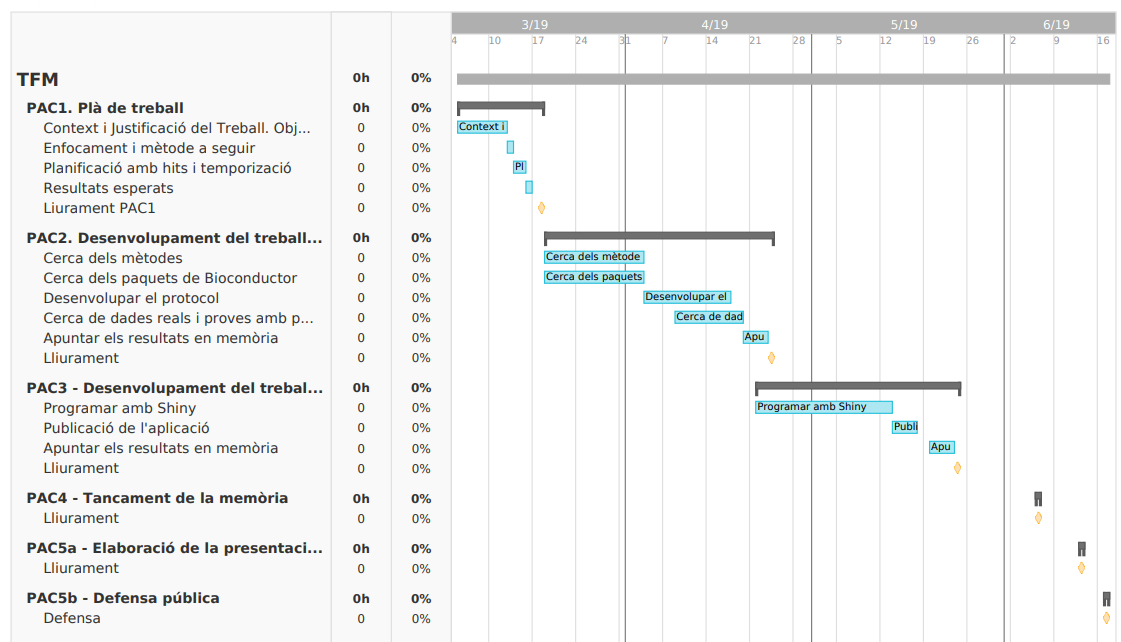
\includegraphics[width=0.9\textwidth]{figures/GanttPlot}
\end{figure}

Els treballs previstos pel pla docent i realitzats i entregats a temps eren els següents: 

\begin{center}
\begin{tabular}{||c | l | c | c||} 
\hline
Activitat & Nom d'activitat & Data d'inici & Data d'entrega \\ [0.5ex] 
\hline\hline
PAC0 & Definició dels continguts del treball & 20/02/19 & 04/03/2019 \\ 
\hline
PAC1 & Pla de treball & 05/03/19 & 18/03/19 \\
\hline
PAC2 & Desenvolupament del treball - Fase 1 & 19/03/19 & 4/04/19 \\
\hline
PAC3 & Desenvolupament del treball - Fase 2 & 25/04/19 & 20/05/19 \\
\hline
PAC4 & Tancament de la memòria & 21/05/19 & 05/06/19 \\
\hline
\end{tabular}
\end{center}

\section{Breu sumari dels productes obtinguts}

El producte central obtingut és l'aplicació Shiny que actualment es pot descarregar del meu repositori a Github (veure l'apartat instal·lació de l'aplicació). Al mateix repositori es pot trobar tot el material relacionat amb la creació de l'aplicació: els arxius de latex per a les proves d'avaluació continuada, les captures de pantalla utilitzades en aquestes PACs, també el paquet modificat \helvetica(pathview) que es diu \helvetica{pathviewPatched} i que permet guardar les imatges de les rutes al directori especificat.

\section{Breu descripció dels capítols del treball}

Al primer capítol més teòric presentaré els mètodes més rellevants per a l’anàlisi de les rutes. Començaré però amb el context d'investigació de l'expressió genètica i més específicament amb l'anàlisi de microarrays per poder situar millor l'anàlisi biològica de les rutes. Donades les dades de l'experiment explicaré breument quins resultats habitualment se’n deriven. Veurem que aquests resultats són la llista de gens diferencialment expressats i la magnitud d'expressio diferencial mesurada via \textit{\gls{logRatio}} per tots els gens. 

Seguidament investigaré quines estratègies existeixen per dur a terme l'anàlisi de les rutes. Aquí identificaré tres estratègies generals: l'anàlisi \gls{ORA} (Over-Representation Analisis), \gls{FCS} (Functional Class Scoring) i l'anàlisi topològica de les rutes. Veurem que aquestes anàlisis accepten com a dades d'entrada els resultats obtinguts via \textit{microarrays} descrits anteriorment. Per poder fer ús d'aquestes dades però és necessari anotar els gens de l'experiment. Per aquest motiu presentaré les tres bases de dades més rellevants per anotar els gens amb l’objectiu de fer l’anàlisi de les rutes: \gls{GO}, \gls{KEGG} i Reactome.

Finalment parlaré sobre els mètodes \gls{ORA} i \gls{GSEA} més detalladament concentrant-me especialment en els resultat que proporcionen. També descriure breument les visualitzacions possibles de les rutes. Per acabar presentaré el protocol que utilitzaré per crear l'aplicació.

Tot seguit explicaré els paquets del \gls{Bioconductor} per dur a terme l'anàlisi descrita al capítol anterior i la manera amb la qual he fet l'aplicació accessible. Veurem que al moment de redacció d'aquesta memòria l'aplicació pot ser descarregada de GitHub utilitzant el paquet \helvetica{devtools} de R. S'intentarà però habilitar l'aplicació per a internet utilitzant el servidor de l'àrea d'estadística i bioinformàtica. 

A continuació presentaré l'aplicació. Aquí utilitzaré les dades del paquet \helvetica{clusterProfiler} per mostrar el funcionament de l'aplicació: des de la pujada de les dades fins a l’obtenció de les representacions gràfiques.

Després intentaré validar l'aplicació. Parlaré dels problemes a l'hora de trobar les dades preprocessades i presentaré les dades amb les que en faig l’intent i em concentraré més en l'estudi de l'expressió gènica dels ratolins modificats genèticament de tal manera que el seu gen Zbtb7b està silenciat. Veurem que els resultats obtinguts amb l'aplicació s'assemblen als resultats descrits al \textit{paper} original. 

Per acabar redactaré les conlusions del meu treball.
\chapter{Marc teòric}

\section{Dades d'expressió genètica}
Les dades d'entrada per a l'anàlisi de les rutes provenen típicament de l'anàlisi de \textit{microarrays} d'ADN, que produeix dades d'expressió de $m$ gens (variables) per a $n$ mARN mostres (observacions). Les dades com aquestes poden resultar d'un estudi d'investigació sobre efectes d'una proteïna com per exemple a l'estudi de \cite{li2017zbtb7b} on s'investiga la correlació entre la proteïna Zbtb7b (Zinc finger and BTB domain-containing protein 7B) i la formació de teixit adipós marró i beix i d'aquesta manera influeix sobre fisiologia metabòlica. En aquest cas l'objectiu és comparar teixits de dos ratolins un de tipus salvatge i l'altre amb el gen ZBTB7B silenciat i investigar quins gens són diferencialment expressats entre aquestes mostres biològiques. 

Al gràfic següent veiem l'estructura habitual d'un experiment de \textit{Microarray} \cite{plaPID00192743}:

\begin{figure}[H]
\centering
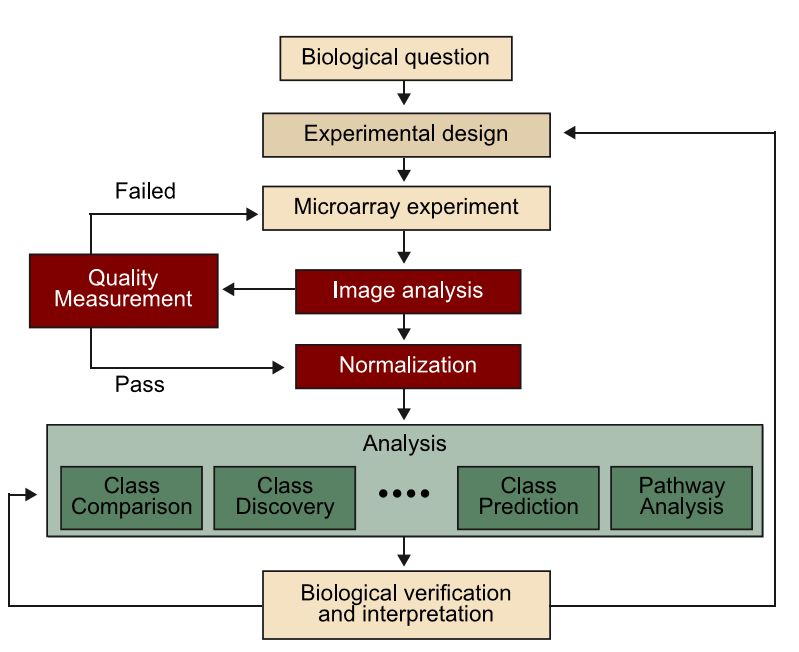
\includegraphics[width=0.9\textwidth]{figures/Pipeline_Microarray.jpg} 
\caption{El procès d'anàlisi de microarrays.}
\end{figure}

El \textit{pipeline} de l'anàlisi consisteix doncs en el plantejament d'una pregunta i un disseny experimental a partir del qual es fa l'experiment de \textit{microarrays}. Els productes de l'experiment són bàsicament les imatges d'intensitats que es tradueixen als valors numèrics. Habitualment aquests valors són encara \textit{raw values} i han de ser processats adequadament. Aquest processament inclou el control de qualitat de les imatges i la normalització dels valors d'intensitat per reduir la variabilitat tècnica. Finalment les dades normalitzades s'utilitzen per a l'anàlisi estadística. Habitualment la mesura natural per comparar les mostres és el \textit{logRatio} el qual podem denominar alternativament \textit{\gls{logFC}} on \textit{FC} es refereix a \textit{fold change}. Hi ha diversos tests estadístics per comprovar les diferències entre les mostres. En el cas de l'array d'un color podem fer servir tant els mètodes paramètrics -com ara el test T o els mètodes del modelatge lineal-, com els mètodes noparamètrics -com ara la proba de Mann-Whitney. El test adequat dependrà bàsicament de la distribució de les dades. El resultat d'aquest anàlisi serveix com a base per a la interpretació biològica dels resultats de l'experiment. Per poder donar sentit a les dades d'expressió i de l'anàlisi estadístic al nivell de gens és imprescindible fer una anàlisi a nivell de les categories de gens o les rutes. Per aquesta anàlisi es necessita, com ho veurem a l'apartat següent, una llista ordenada de les expressions relatives (\textit{\gls{logFC}}) i una subllista de gens que hem identificat mitjançant els tests estadístics com a diferencialment expressats.

En aquest treball m'ocupo de l'últim pas de l'experiment descrit, més específicament de l'anàlisi de rutes (\textit{Pathway analysis}).

La vista general de l'anàlisi de les rutes ofereix el gràfic següent \cite{khatri2012ten}:

\begin{figure}[H]
\centering
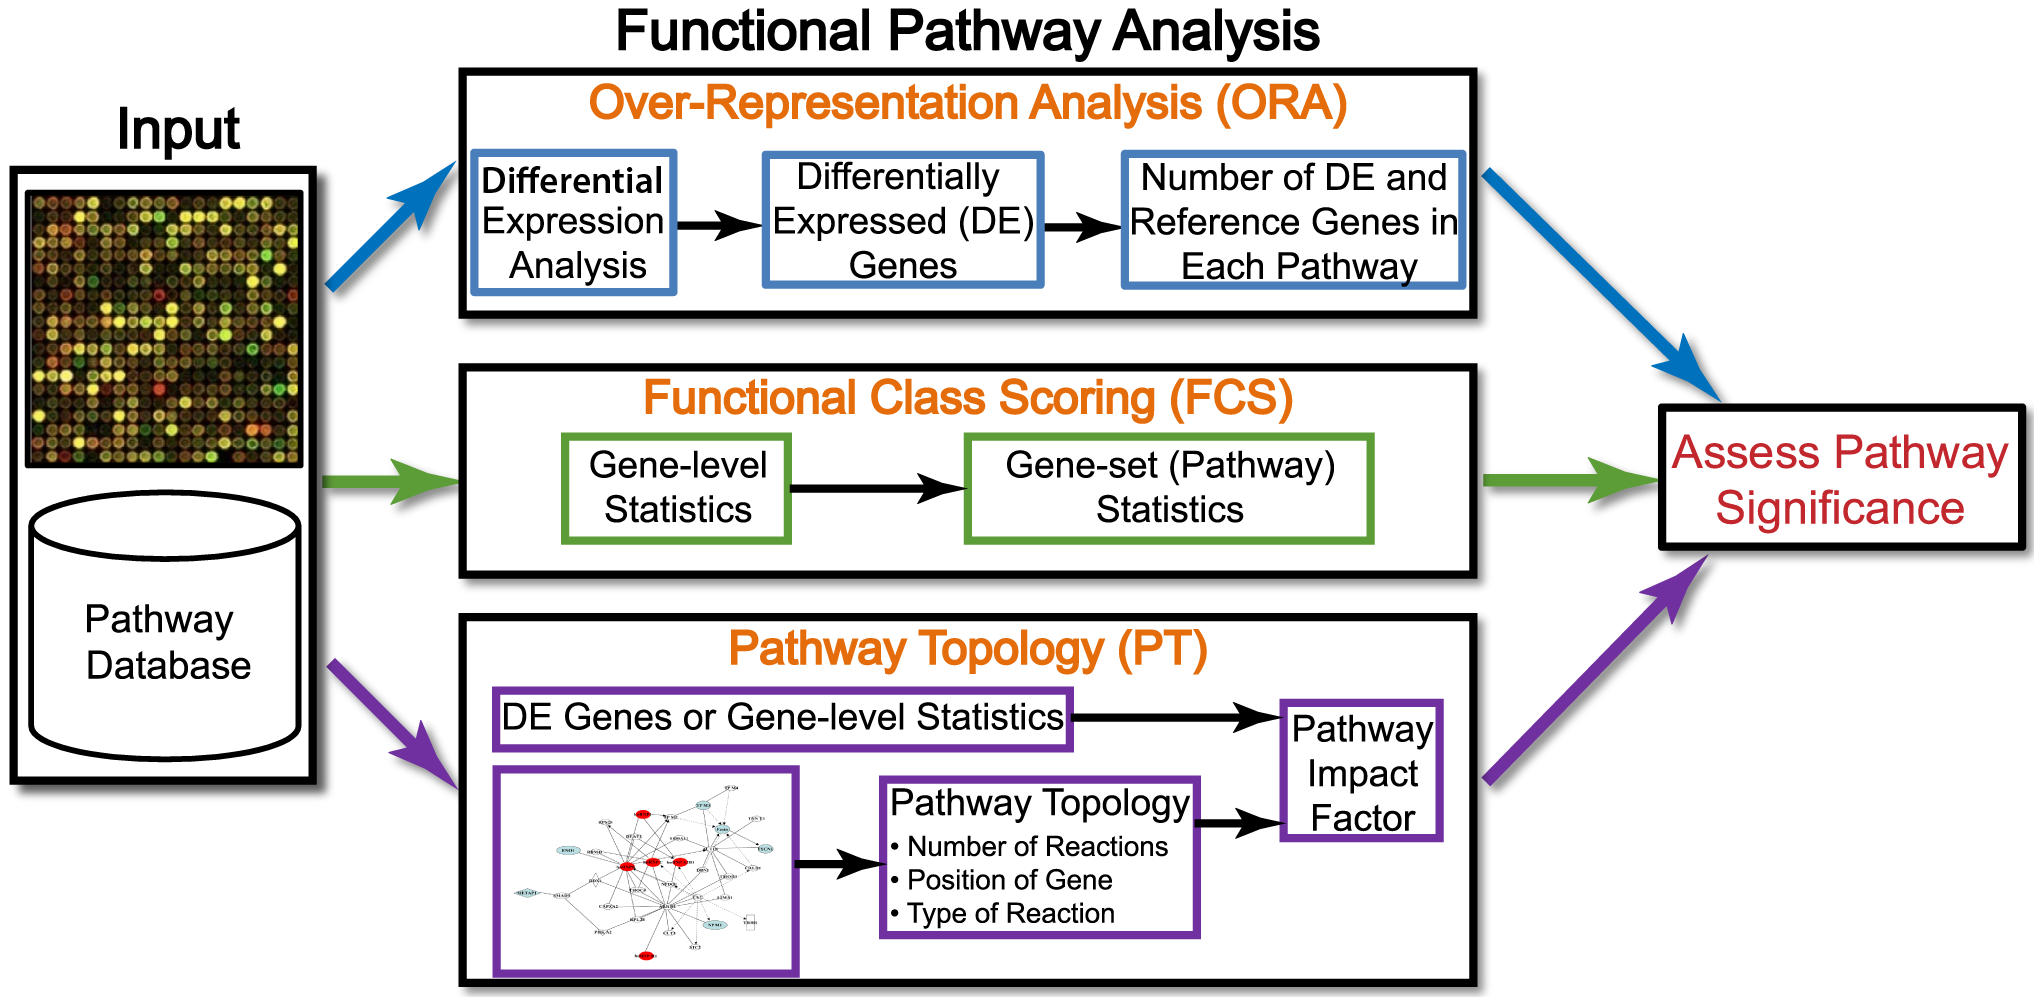
\includegraphics[width=0.9\textwidth]{figures/Pipeline_Pathway.png} 
\caption{El procés d'anàlisi de les rutes.}
\end{figure}

A part de les dades d'expressió, de les quals he parlat anteriorment, l'anàlisi requereix com a \textit{input} també la base de dades de les rutes. De les dades que utilitzaré a la meva aplicació en parlaré a la secció següent. Per ara és important entendre que els resultats d'expressió s'anoten a les bases de dades existents per comprovar si els gens sobre o sotaexpressats pertanyen a unes rutes específiques. Per comprovar aquesta, o millor dit, aquestes hipòtesis (per que hi haurà hipòtesis múltiples) s'han establert tres grups de mètodes:

\begin{itemize}
\item \textbf{Over-Representation Anaysis (\gls{ORA})}.
Aquesta anàlisi necessita la preselecció dels gens diferencialment expressats (DE) i compara la freqüència dels gens de la ruta d'interès en la mostra dels gens diferencialment expressats i la freqüència dels gens de la ruta a la distribució de fons (\cite{boyle2004go}. 
\item \textbf{Functional Class Scoring (\gls{FCS})}
Per a aquesta anàlisi no necessitem cap preselecció dels gens diferencialment expressats (DE) sinó ja és suficient amb tenir les estadístiques a nivell de gens, que al cas de l'aplicació és el \textit{\gls{logFC}}. Hi ha diversos mètodes que generen una estadística per a tot el conjunt de gens d'una ruta i la comparen amb una distribució teòrica per a contrastar la hipòtesi nul·la. Els mètodes es diferencien bàsicament en el càlcul de la puntuació d'enriquiment que poden incloure l'estadística de Kolmogorov-Smornov, la suma, mitjana o mediana d'estadístiques al nivell de gens etc. \cite{khatri2012ten}. O bé es poden diferenciar en el càlcul de la distribució teòrica: aquí alguns mètodes utilitzen la permutació de les mostres o de gens, cosa que implica dues hipòtesis diferents. 
\item \textbf{Pathway Topology (\gls{PT})}.
Aquest mètode enfoca la posició dels gens diferencialment expressats en la ruta i d'aquesta manera utilitza el coneixement de les bases de dades més àmpliament. Per exemple, si una ruta està activada per un sol producte genètic o mitjançant un receptor i si aquesta proteïna particular no està produïda, la ruta estarà molt afectada, o fins i tot apagada. Més específicament, si el receptor d'insulina no és en la ruta d'insulina (\url{https://www.genome.jp/dbget-bin/www_bget?hsa04910}) tota la ruta serà desactivada (\cite{tarca2008novel}). D'altra banda, si un nombre de gens està involucrat en la ruta però apareixen riu abaix el seu efecte podria ser menys important. A més a més, també el nombre de connexions amb altres gens a la ruta podria ser important \cite{rahnenfuhrer2004calculating}. O fins i tot les estadístiques que incorporen factors diferents com ara la posició, el tipus d'interacció etc. \cite{draghici2007systems}. Aquesta idea l'he implementat en l'aplicació afegint les rutes dibuixades de \gls{KEGG} i Reactome, on els gens estan emfatitzats d'acord amb els \textit{\gls{logFC}s} obtinguts mitjançant l'experiment.

En els capítols següents precisaré més formalment els mètodes d'\gls{ORA} i \gls{GSEA} i també descriuré algunes possibilitats per visualitzar les dependències de gens dins de les rutes específiques i també les relacions entre les rutes diferencialment expressades.

\end{itemize}


\section{Annotació dels gens}

Com veurem més endavant per a l’anàlisi de les rutes és imprescindible tenir com a referència les anotacions dels gens. Per a l’aplicació he utilitzat tres bases de dades: Gene Onthology (GO), Kyoto Encyclopedia of Genes and Genomes (KEGG) i Reactome. \helvetica{clusterProfiler} també inclou WikiPathways però per raons de temps he decidit centrar-me només en les tres mencionades anteriorment. Aquestes bases de dades no són però úniques. N'hi ha també altres com per exemple \textit{Pathway Studio pathways} o \textit{IPA} amb l’inconvenient que són comercials i no gratuïtes. 

\subsection{Gene ontology}
Gene Ontology \cite{gene2004gene} dona tan un vocabulari estructurat i controlat (ontologies) com la classificació que cobreix alguns dominis de la biologia molecular i cel·lular. És una base de dades gratuïta per a anotació de gens, el seu producte i les seqüències. El projecte \gls{GO} proporciona ontologies per a descriure els atributs dels productes de gens als tres dominis separats de la biologia molecular:
\begin{enumerate}
\item \textbf{Molecular Function (MF)}. Aquest domini descriu les activitats a nivell molecular. És important entendre que el terme ``molecular function'' representa més les activitats que no pas les entitats (com per exemple molècules o complexos) que fan aquestes accions, i a més a més no especifiquen quan o a quin context l'acció té lloc. Un exemple podria ser \textit{catalytic activity} o un terme més específic \textit{adenylate cyclase activity}.
\item \textbf{Biological Process (BP)}. Aquest domini descriu els objectius biològics aconseguits per una de les funcions moleculars o un conjunt d’elles. Un exemple d'un procés biològic ampli podria ser \textit{DNA repair}. Un exemple més específic podria ser \textit{pyrimidine nucleobase biosynthetic process}. 
\item \textbf{Cellular Component (CC)}. EL CC descriu l'emplaçament al nivell d'estructures subcel·lulars (com \textit{mitocondri}) i els complexos macromoleculars (com \textit{ribisomes}) on el producte de gen fa la seva funció.
\end{enumerate}

Dins de cada ontologia, els termes tenen tan una definició de text com un identificador únic. El vocabulari està estructurat en una classificació que manté les relacions ``is-a'' i ``part-of'' i ``regulates''. Aquestes relacions les descric amb més detall més endavant en la secció dedicada al gràfic acíclic de \gls{GO} termes.

\subsection{\gls{KEGG}}
La base de dades \gls{KEGG} és la col·lecció dels mapes dibuixats manualment que representen el coneixement sobre interacció molecular dividit en set dominis principals:
\begin{enumerate}
\item Metabolism
\item Genetic Information Processing
\item Environmental Information Processing
\item Cellular Processes
\item Organismal Systems
\item Human Deseases
\item Drug Development
\end{enumerate}

Els mapes són dibuixats amb un software específic (KegSketch) que genera un arxiu KGML+. Aquest arxiu és un arxiu SVG que conté els objectes gràfics que són associats amb els objectes \gls{KEGG}. Els objectes gràfics bàsics de les rutes \gls{KEGG} són:
\begin{itemize}
\item caixes: gens o el seu producte
\item cercles: altres molècules
\item línies: reaccions
\end{itemize}
El significat més detallat d'aquests elements el presentaré a la secció dedicada a les rutes \gls{KEGG}.

\subsection{Reactome}

Reactome és una base de dades gratuïtament accessible i manualment curada per a reaccions i rutes biològiques. Al centre de Reactome hi ha reaccions que es defineixen com qualsevol esdeveniment molecular com ara unió, fosforització, catàlisi bioquímic, transport molecular o esdeveniments moleculars espontanis. Aquestes reaccions involucren qualsevol molècula, però més típicament passen entre proteïnes i les molècules petites. Encara que els mapes de Reactome disponibles online contenen una relació entre les molècules més detallada, el paquet de \gls{Bioconductor} que utilitzaré per generar els mapes visualitza només la connexió bàsica entre els gens. 

\section{\gls{ORA}}

L'anàlisi de sobreexpressió és una tècnica d'identificació de les rutes significativament enriquides en la mostra d'interès. 

El paper original que se cita habitualment quan es parla d'anàlisi d'expressió genètica és de \cite{boyle2004go}. El mètode estadístic descrit consisteix bàsicament en els passos següents:

\begin{enumerate}
\item \textbf{De tots els gens de la mostra seleccionar un grup de gens que es considera que són significativament expressats.}

Els criteris de selecció poden basar-se en \textit{\gls{logRatio}s} i/o en el valor de p provinent d'un test estadístic. \textit{\gls{logRatio}s} donen la magnitud amb la qual un gen és sobre o sotaexpressat. Les diferències entre els grups però són el resultat d'un procés estocàstic i per tant hem d'intentar de minimitzar el risc de prendre decisions falses. El valor de p representa la probabilitat d'aquest risc i per tant dona certa confiança sobre la significació de les diferències observades.

\item \textbf{Determinar si algunes rutes anoten la llista especificada de gens amb la freqüència més alta que la que s’esperaria per casualitat.} 

El test estadístic es basa en la distribució hipergeomètrica: 

$$p = 1 - \displaystyle\sum_{i = 0}^{k-1}\frac{{M \choose i}{{N-M} \choose {n-i}}} {{N \choose n}}$$

Aquesta equació $N$ és el nombre total de gens en la distribució de fons, $M$ és el nombre de gens dins d'aquesta distribució que són anotats a la ruta d'interès, $n$ és el nombre total en la llista especificada de gens i $k$ és el nombre de gens dins d'aquesta llista que són anotats a la ruta. La distribució de fons pot ser o bé tots els gens en la base de dades d'anotació o bé tots els gens de l'experiment.

El valor de P obtingut amb aquesta fórmula dona la probabilitat de veure el nombre $x$ de gens de la llista relacionats amb la ruta específica en la llista del nombre total de gens $n$ donat la proporció de gens relacionats amb aquesta ruta en la distribució de fons.
\end{enumerate}

L'aplicació utilitza aquesta idea i calcula una taula amb els camps següents:


\begin{itemize}
\item \underline{Description}. El nom del terme \gls{GO};
\item \underline{GeneRatio}. El quocient $\frac{M}{N}$ on $M$ és el nombre dels gens diferencialment expressats que pertanyen al conjunt de gens i $N$ és el nombre total dels gens diferencialment expressats .
\item \underline{BgRatio}. El quocient: $\frac{k}{n}$ on $k$ és el nombre dels gens del conjunt d'interès en la distribució de fons i n és el nombre total dels gens en la distribució de fons;
\item \underline{pvalue}. Valor de p basat en la distribució hipergeomètrica descrita anteriorment.
\item \underline{p.adjust}. El valor de P ajustat. L'usuari pot seleccionar el mètode d'ajustmanent.
\end{itemize}

Debilitats d'aquest mètode són les següents:
\begin{itemize}
\item Les estadístiques utilitzades pel mètode ORA, com ara la distribució hipergeomètrica, són independents dels canvis mesurats. Això vol dir que aquests tests ignoren tots els valors associats amb ells com ara les intensitats (logRatios).
\item Típicament ORA utilitza només els gens més significatius i descarta els altres.
\item ORA tracta cada gen igual i per tant assumeix que tots els gens són independents els uns dels altres.
\item ORA assumeix que totes les rutes són independents l’una de l’altra.
\end{itemize}


\section{\gls{GSEA}}

Amb l'anàlisi \gls{GSEA} podem analitzar els resultats d'un experiment d'expressió per a dos grups. Aquí els gens són ordenats basant-se en la correlació entre la seva expressió i la separació entre les classes. Aquest llistat ordenat $L$ el podem crear utilitzant els \textit{\gls{logRatio}s}.

Donat el conjunt definit dels gens $S$, que pertanyen per exemple al mateix terme de Gene Ontology, l'objectiu de GSEA és determinar si els membres de $S$ són distribuïts aleatòriament en el $L$ o es troben més al cap o a la cua. S'esperaria que els gens relacionats amb la separació fenotípica mostrin aquesta última distribució. 

L'anàlisi \gls{GSEA} consisteix en tres passos \cite{subramanian2005gene}:

\begin{enumerate}
\item Càlcul de la puntuació d’enriquiment (\textit{\gls{ES}: Enrichment Score}). La puntuació està calculada anant per la llista i augmentant la suma corrent sempre quan es troba un gen que pertany a $S$ o, al contrari, restant-la quan el gen no forma part del conjunt $S$. La puntuació és la desviació màxima del zero observada en aquet camí. L'estadística obtinguda és l’estadística de Kolmogorov-Smirnov amb pesos.

\item Estimació del nivell de significació per a la puntuació \textit{\gls{ES}}. El valor de P nominal es pot obtenir mitjançant o bé la permutació de les classes o bé la permutació de gens, on l'estadística \textit{\gls{ES}} observada es compara amb la distribució obtinguda amb permutació. Els dos modes de permutació comproven hipòtesis diferents. Mentre la permutació de gens comprova la hipòtesi que \textit{els gens en la ruta com a màxim són diferencialment expressats com els gens fora de la ruta},
la permutació de les mostres implica la hipòtesi que cap de gens en la ruta són diferencialment expressats. Es diferencia doncs en el tractament dels gens fora de la ruta. A l'aplicació es fa ús de la permutació dels gens a causa bàsicament de la selecció dels paquets de \gls{Bioconductor} per a l’aplicació.


\item Càlcul del valor de P ajustat. El valor de P nominal s'ajusta per controlar l'error global que es produeix com a resultat de les comparacions múltiples.
\end{enumerate}

\begin{figure}[H]
\centering
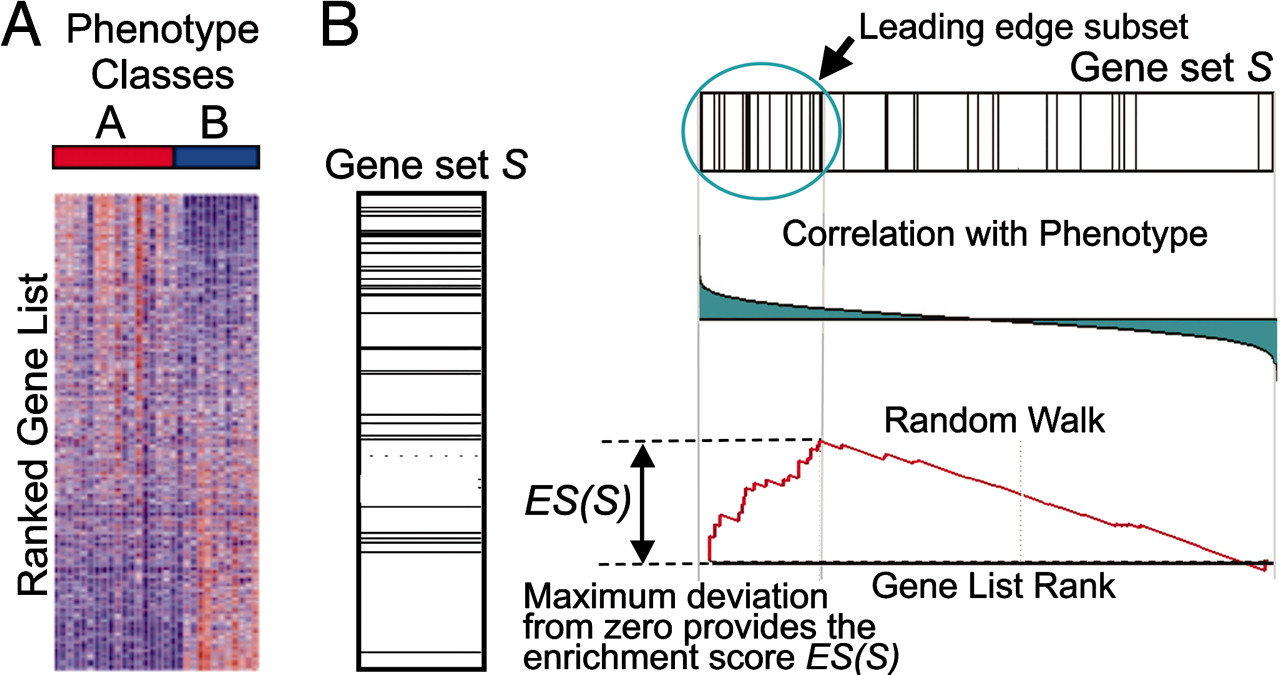
\includegraphics[width=0.9\textwidth]{figures/GSEA_Method.jpg} 
\caption{El mètode \gls{GSEA}}
\end{figure}

L'aplicació que he desenvolupat agafa aquesta idea i calcula la taula que inclou les estadístiques següents:

\begin{itemize}
\item \underline{enrichmentScore}. Enrichment score per al conjunt dels gens. Amb altres paraules: el grau amb el qual el conjunt dels gens està sobreexpressat a dalt o a baix del llistat ordenat dels gens en les dades d'expressió.
\item \underline{NES}. Normalized enrichment score. La puntuació per al conjunt de gens després de ser normalitzat tenint en compte tots els conjunts de gens analitzats (la seva mida i la seva correlació amb les dades d'expressió). Aquesta puntuació ajuda a comparar els resultats entre els conjunts de gens.
\item \underline{pvalue}.El valor de p nominal.
\item \underline{p.adjust}. El valor de p ajustat.
\item \underline{leading\_edge}
\begin{itemize}
\item \underline{Tags}. El percentatge de les ocurrències de gens del conjunt específic abans (per als ES positius) o després (per als ES negatius) del cim en la puntuació corrent d'enriquiment. Aquest valor indica el percentatge dels gens que contribueixen a la puntuació d'enriquement. 
\item \underline{List}. El percentatge dels gens en el llistat ordenat de tots els gens abans o després del pic en la puntuació corrent d'enriquiment. Aquest valor ens indica on es produeix exactament el pic. 
\item \underline{Signal}. La fortalesa del senyal d'enriquiment que combina els dos valors anteriors.
\end{itemize}
\item \underline{rank}. La posició del pic en la llista ordenada dels gens. Els conjunts dels gens més interessants assoleixen el seu màxim o bé al principi o al final de la llista ordenada. Vol dir que tenen aquest valor o bé molt baix o bé molt alt.
\end{itemize}

Encara que GSEA és una millora respecte a ORA, aquest mètode també té les seves debilitats: 
\begin{itemize}
\item Tal com l’anàlisi ORA, també GSEA assumeix que les rutes són independents.
\item GSEA utilitza els canvis d’expressió gènica dins de la ruta específica i descarta els canvis d’altres anàlisis. Per exemple, agafem dos gens A i B, que canvien dues vegades l’un (2-fold) i 20 vegades l’altre (20-fold) respectivament. Fins que aquests gens tinguin el mateix rang comparat amb altres gens de la ruta, GSEA els tractarà igual, encara que seria preferible donar més pes al gen B.
\end{itemize}

\section{Anàlisi topològic de les rutes}
Tan \gls{ORA} com \gls{GSEA} no visualitzen les relacions entre les rutes i entre els gens dins de les rutes. Els avenços en anotació manual de les bases de dades disponibles (\gls{GO}, \gls{KEGG} i Reactome) contenen però aquesta informació i l'aplicació, gràcies al paquet \helvetica{clusterProfiler}, hi treu l'avantatge i visualitza aquestes relacions més detalladament. 

\subsection{El mapa d'enriquement}

L’anàlisi \gls{ORA} resulta en una llista de les rutes significativament enriquides. Els gens dins dels conjunts o les rutes poden encavalcar i descriuen gairebé conceptes biològics idèntics \cite{merico2010enrichment}. Aquest problema de redundància és més evident als conceptes que són organitzats jeràrquicament, com és el cas dels conceptes de la base da dades \gls{GO}. El mapa d’enriquiment redueix la redundància als conjunts de gens. Els conjunt de gens estan representats com a nodes els radis dels quals són proporcionalment relacionats amb el nombre de gens que formen part d’aquests conjunts. Els cantells indiquen els nodes que tenen gens compartits, on el seu gruix depèn del nombre de gens compartits. A més a més, es pot utilitzar el color dels nodes per representar una altra dimensió com ara el nivell de significació expressat per el valor de P. Si no hi ha cap gen compartit entre els conceptes (o rutes) els nodes no són connectats via cantells. Aquest mètode de representació és molt útil per poder reduir/simplificar la informació obtinguda mitjançant els mètodes \gls{ORA} o \gls{GSEA} i per tant m’he posat l’objectiu també d’implementar-lo a l’aplicació. 

\subsection{\gls{Gene-Concept-Network}}

L'anàlisi \gls{ORA} no visualitza per si sola els gens que contribueixen al fet que la ruta sigui diferencialment expressada. Amb la xarxa de gens-concepte es pretén visualitzar els gens al voltant dels conceptes on els gens poden ser connectats amb rutes (conceptes) diferents. D'aquesta manera es fa possible identificar les associacions biològiques més complexes entre les rutes mitjançant els gens. 

\subsection{\gls{GO-Plot}}
%Per a mès informació http://geneontology.org/docs/ontology-relations/

El gràfic de \gls{GO} està organitzat com direccional acíclic gràfic (Directed Acyclic Graph). Una manera útil de veure els resultats és mirar com els termes \gls{GO} estan distribuïts per aquest gràfic. L'aplicació ensenya el gràfic \gls{GO} induït pels gens més significatius. El gràfic mostra tres relacions possibles entre les rutes: 
\begin{enumerate}
\item \textit{is a}: Si dèiem que A \textit{is a} B, volem dir que A és un subtip de B. Per exemple el cicle mitòtic de la cèl·lula \textit{is a} cicle de la cèl·lula. 
\item \textit{part of}: Aquesta relació s'utilitza per representar la relació entre una part i el tot. Aquesta relació entre A i B existeix només si B és necessàriament una part d'A: quan B existeix, ho fa només com una part de B i la presència de B implica la presència d’A.
\item \textit{regulates}: La relació descriu el cas on un procés afecta directament la manifestació de l'altre procés.
\end{enumerate}

Els conceptes al llarg del gràfic estan marcats amb color depenent de si són estadísticament significatius o no.

\subsection{\gls{KEGG Pathway}}
%Per a més informació sobre l'anotació https://www.genome.jp/kegg/document/help_pathway.html
Aquest gràfic mostra les relacions entre els gens dins de la ruta específica. Els gens són remarcats amb el color depenent de l'expressió diferencial mesurada amb LogRatios. Per poder interpretar el gràfic és útil tenir present l'anotació següent:

\begin{figure}[H]
\centering
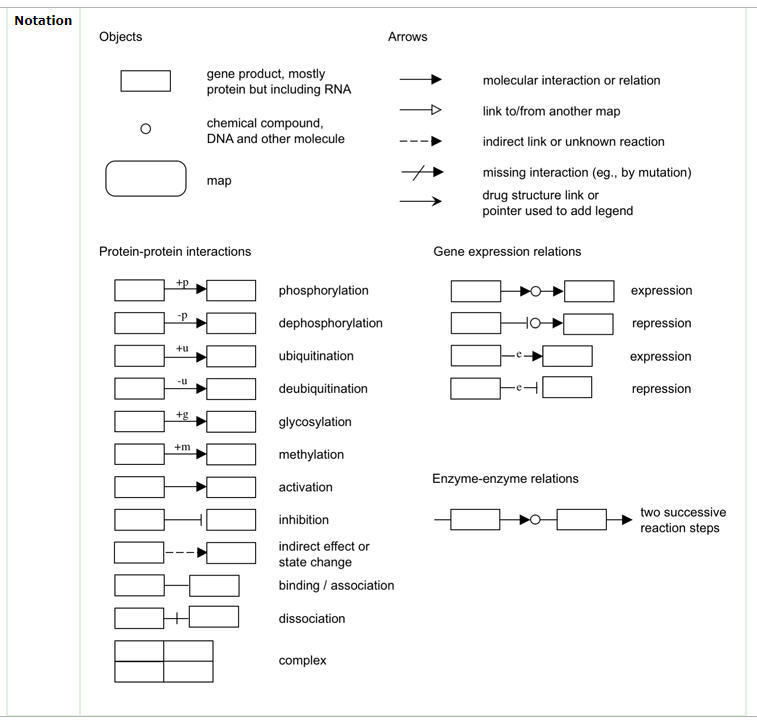
\includegraphics[width=0.9\textwidth]{figures/Annotation_KEGG.jpg} 
\caption{L'anotació de les relacions dins de les rutes \gls{KEGG}}
\end{figure}

\subsection{Reactome Pathway}

Les rutes de Rectome són similares a les rutes de \gls{KEGG}. La seva implementació amb \gls{Bioconductor}, com ho veurem properament, no visualitza les rutes originals mostrades per \href{https://reactome.org/PathwayBrowser/}{Pathway Browser} de Reactome. La visualització amb al paquet \helvetica{ReactomePA} és més modesta i ofereix només les relacions nominals sense mostrar direccionalitat, com ho fa el gràfic de la ruta original de Reactome. Tot i així podem identificar quantes connexions amb altres gens de la ruta tenen els gens diferencialment expressats i d'aquesta manera intuir la seva importància relativa. 

En canvi a Goplot i les rutes \gls{KEGG} les relacions entre els gens dins les rutes Reactome són més senzilles. Aquí les relacions estan mostrades només amb les línies, on es pot interpretar només la distància entre els gens. 
%https://reactome.org/userguide/pathway-browser

\section{Desenvolupament del protocol}

Tenint en compte el marc teòric he intentat dissenyar l'aplicació de tal manera que ofereixi els mètodes \gls{ORA}, \gls{GSEA} i algunes visualitzacions de la topografia de les rutes. Tan se val amb quina base de dades l'usuari anoti les dades d'expressió, ja que l'usuari podrà decidir quin mètode vol aplicar. En el millor dels casos l'usuari faria els dos mètodes ORA i GSEA. Això implicaria la disponibilitat de dos arxius: l'arxiu amb tots els gens (Universe) i l'arxiu amb el grup de gens diferencialment expressats (Gene set). Si l'usuari vol fer només l'anpalisi \gls{GSEA} haurà de pujar només l'arxiu amb tots els gens. Una vegada seleccionada l'estratègia l'usuari puja els arxius necessaris i genera el resultat de \gls{ORA} i/o \gls{GSEA} aplicant uns criteris com ara selecció d'ontologia en ORA, valor de P com al filtre de visualització de les rutes més significatives, i el mètode d'ajustament.

\begin{figure}[H]
\centering
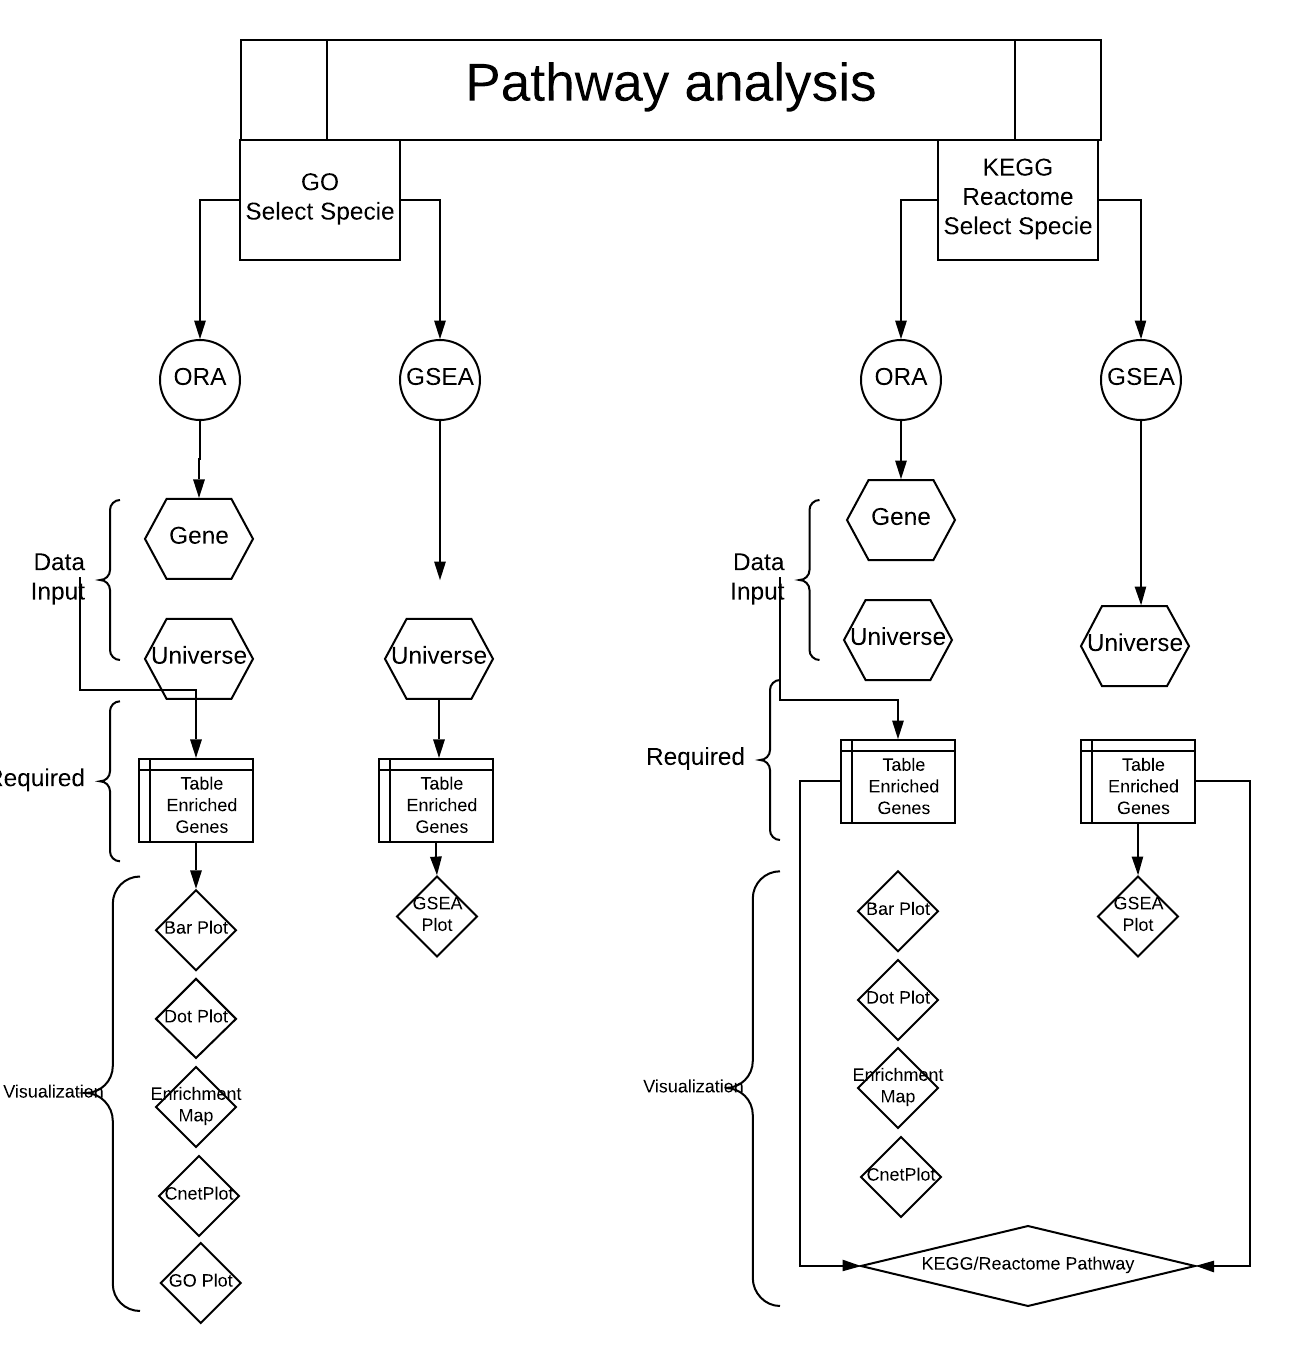
\includegraphics[width=.9\textwidth]{figures/LucidChart} 
\caption{Lucidchart per a l'aplicació}
\end{figure}

D'aquí podem definir per exemple el protocol:
\begin{enumerate}
\item Decidir quin anàlisi vol fer: \gls{GO}, \gls{KEGG} o Reactome
\item Seleccionar l'espècie de referència
\item Decidir quin mètode vol implementar: \gls{ORA} o \gls{GSEA} i respectivament pujar les dades necessàries.

$\rightarrow$ Per a anàlisi \gls{GO} tots dos arxius són necessaris: Gens Seleccionats (Gene) i Tots els gens (Universe). 

$\rightarrow$ Per a l'anàlisi \gls{KEGG} o Reactome les dades necessàries varien: Pel mètode \gls{ORA} l'arxiu amb els gens seleccionats és suficient. Dos arxius són necessaris pel mètode \gls{GSEA}.
\item En el cas que vulguem fer l’anàlisi \gls{ORA} seleccionar a l'apartat corresponent (\gls{GO}, \gls{KEGG} o Reactome) la pestanya \gls{ORA} i definir els criteris.

$\rightarrow$ Els gràfics: \gls{Bar-Plot}, \gls{Dot-Plot}, \gls{Enrichment Map}, Cnet Plot, GO Plot (en cas d'anàlisi \gls{GO}) i els gràfics de les rutes (\gls{KEGG}/Reactome) es calculen automàticament

\item En el cas que vulguem fer l'anàlisi \gls{GSEA} seleccionar a l'apartat corresponent (\gls{GO}, \gls{KEGG} o Reactome) la pestanya \gls{GSEA} i definir els criteris.

$\rightarrow$ El gràfic GSEA es genera automàticament. Es pot elegir la ruta mitjançant un menú desplegable.

\end{enumerate}

\chapter{Tractament bioinformàtic}

\section{Cerca dels paquets de \gls{Bioconductor}}
El \gls{Bioconductor} ofereix molts paquets per dur a terme l'anàlisi de les rutes implementant algoritmes diferents a l'hora de calcular les estadístiques de les anàlisis \gls{ORA} i \gls{GSEA}. La cerca s'ha reduït a tres paquets principals: \helvetica{clusterProfiler}, \helvetica{ReactomePA} i \helvetica{pathview}. D'aquests tres paquets el paquet \helvetica{clusterProfiler} és el més complet i integra els mètodes per dur a terme l'anàlisi de les rutes basant-se en les bases de dades \gls{GO}, \gls{KEGG} i Reactome. Els dos mètodes principals són \gls{ORA} i \gls{GSEA}. També inclou les possibilitats de visualització dels resultats suficients per considerar l'anàlisi de les rutes completa. Notem però que el test de permutació a l'anàlisi \gls{GSEA} implementat per clusterPrifiler es basa en la permutació dels gens i no de les mostres com originalment és proposat per \cite{subramanian2005gene}.

Els paquets i les seves funcions per generar els resultats són els següents: 

\begin{table}[H]
\begin{adjustbox}{width=1\textwidth}
\small
\begin{tabular}{|| c | c | l | c | c ||} 
\hline
Base de dades & Mètode & Paquet \gls{Bioconductor} & Funció & Observació \\ [0.5ex] 
\hline\hline
\gls{GO} & \gls{ORA} & clusterProfiler & enrichGO() & Només 7 espècies disponibles \\ 
\hline
GO & GSEA & clusterProfiler & gseGO() & Permutació de gens \\
\hline
GO & \gls{Bar-Plot} & enrichplot & barplot() & Necessita l'objecte del class enrichResult \\
\hline
GO & \gls{Enrichment Map} & enrichplot & emapplot() & Necessita l'objecte del class enrichResult \\
\hline
GO & \gls{Gene-Concept-Network} & enrichplot & cnetplot() & Necessita l'objecte del class enrichResult \\
\hline
GO & GO directed acyclic graph & enrichplot & goplot() & Necessita l'objecte del class enrichResult \\
\hline\hline
KEGG & ORA & clusterProfiler & enrichKEGG() & Totes les espècies de KEGG \\ 
\hline
KEGG & GSEA & clusterProfiler & gseKEGG() & Permutació de gens \\
\hline
KEGG & \gls{Bar-Plot} & enrichplot & barplot() & Necessita l'objecte del class enrichResult \\
\hline
KEGG & \gls{Enrichment Map} & enrichplot & emapplot() & Necessita l'objecte del class enrichResult \\
\hline
KEGG & \gls{Gene-Concept-Network} & enrichplot & cnetplot() & Necessita l'objecte del class enrichResult \\
\hline
KEGG & Pathway & pathview & pathview() & Cal modificar la funció per guardar els gràfics en el directori temporal \\
\hline\hline
Reactome & ORA & ReactomePA & enrichPathway() & Totes les espècies de KEGG \\ 
\hline
Reactome & GSEA & ReactomePA & gsePathway() & Permutació de gens \\
\hline
Reactome & \gls{Bar-Plot} & enrichplot & barplot() & Necessita l'objecte del class enrichResult \\
\hline
Reactome & \gls{Enrichment Map} & enrichplot & emapplot() & Necessita l'objecte del class enrichResult \\
\hline
Reactome & \gls{Gene-Concept-Network} & enrichplot & cnetplot() & Necessita l'objecte del class enrichResult \\
\hline
Reactome & Pathway & ReactomePA & viewPathway() & \\
\hline
\hline
\end{tabular}
\end{adjustbox}
\caption{Resum de les anàlisis disponibles i recursos de \gls{Bioconductor} R} 
\end{table}



\section{Instal·lació de l'aplicació}

La solució més plausible i ràpida era empaquetar tota l'aplicació dins d'un paquet R i fer-la disponible d'aquesta manera en el GitHub. Hi havia també dues opcions més: 

\begin{itemize}
\item Publicar l'aplicació a CRAN
\item Publicar l'aplicació en un servidor Shiny
\end{itemize}
La primera opció, publicació en CRAN, no l’he contemplat encara, perquè la solució no és immediata, sinó que és un procès que no és fàcil i pot tardar fins que el paquet estigui
publicat amb èxit. Com comenta \cite{HWick} \enquote{submitting to CRAN is a lot more work than just providing a version on github, but the vast majority of R users do not install packages from github, because CRAN provides discoverability, ease of installation and a stamp of authenticity. The CRAN submission process can be frustrating, but it’s worthwhile...}. Normalment els paquets han d’estar en perfectes condicions abans d'entregar-los i seran revisats manualmet per un equip de voluntaris. D'aquesta manera l'aplicació no seria avaluable dins del marc temporal previst per al treball de màster. A més a més, considero que podria millorar encara més l'aplicació abans d'entregar-lo.

La segona opció, publicació via Shiny Server, és molt interessant, però implicaria un treball considerable per configurar el servidor. Com que ho faria per primera vegada, no puc assegurar que tot estigui preparat a temps. 

Per tant, el paquet \helvetica{PathwayApp} es pot instal•lar del repositori GitHub seguint els passos següents:

\begin{enumerate}
\item Instal·lar, si encara no està fet, la versió actual de R;

\item Instal·lar, si encara no està fet, el \gls{Bioconductor};

\item Instal·lar, si encara no està fet, el paquet \helvetica{devtools}

\begin{lstlisting}[language=R]
install.packages(``devtools'')
library(devtools)
\end{lstlisting}

\item Instal·lar el paquet \helvetica{PathwayApp}

\begin{lstlisting}[language=R]
devtools::install_github("vdruchkiv/TFM/5_Packages/PathwayApp/PathwayApp")
\end{lstlisting}

\item Iniciar l'aplicació 
\begin{lstlisting}[language=R]
PathwayApp::runPathwayApp()
\end{lstlisting}
\end{enumerate}

La funció \helvetica{runPathwayApp()} iniciarà la comprovació dels paquets necessaris i començarà l'aplicació. Els paquets següents seran instal·lats, si no ho estan ja:

\begin{center}
\begin{tabular}{||c | c ||} 
\hline\hline 
\textbf{Paquet} & \textbf{Font} \\ [0.5ex] 
\hline\hline
clusterProfiler & \gls{Bioconductor} \\
\hline
ReactomePA & \gls{Bioconductor} \\
\hline
pathview & \gls{Bioconductor} \\ 
\hline
pathviewPatched & GitHub vdruchkiv/TFM\\
\hline
dplyr & CRAN \\
\hline 
ggplot2 & CRAN \\
\hline
knitr & CRAN \\
\hline
kableExtra & CRAN \\
\hline
formattable & CRAN \\
\hline
shiny & CRAN \\
\hline 
shinydashboard & CRAN \\ 
\hline
shinyhelper & CRAN \\
\hline 
shinycssloaders & CRAN\\
\hline\hline
\end{tabular}
\end{center}

He decidit no forçar la instal·lació de totes les bases d’anotacions per GO i Reactome. Al servidor sí que ho faria, però per a la instal·lació local podria resultar ser una experiència massa ferragosa, perquè encara que l’usuari necessités per a la seva anàlisi només un genoma anotat específic, hauria d’instal·lar tots els altres innecessàriament; i per tant dedicar més temps a la instal·lació que iniciaria amb la primera crida de la funció; \helvetica{runPathwayApp} i a més a més també ocuparia espai al seu disc dur. Recordem que cada base d’anotació té un pes important. La base de dades org.Mm.eg.db per a ratolí, per exemple, ocuparà aprox. 275 megabytes al disc dur. Si anteriorment les anotacions no són descarades per a l’espècie que l’usuari vol analitzar, l’usuari rebrà un error: \textbf{ERROR: object 'org.Mm.eg.db’ is not found}.

\chapter{L'aplicació}

Després de la instal·lació l'aplicació és completament funcional localment i ofereix l'anàlisi a partir de les bases de dades \gls{GO}, \gls{KEGG} i Reactome. A l'apartat \textbf{Input data} l'usuari primer ha d'indicar l'espècie per a totes tres bases de dades. Per les bases de dades de Reactome l'usuari pot elegir entre Homo Sapiens, Rat, Mouse, Celegans, Yeast, Zebrafish, Fly. Per a l’anàlisi GO, a més de les anteriors, hi ha disponibles aquestes espècies addicionals: Arabidopsis, Bovine, Chicken, Canine, Pig, Rhesus, E coli strain K12, Xenopus, Anopheles, Chimp, Malaria, E coli strain Sakai. Hi ha més espècies disponibles per a l'anàlisis \gls{KEGG}, perquè la funció de \helvetica{culsterProfiler} \helvetica{enrichKEGG()} descarrega les últimes anotacions directament de la base de dades \gls{KEGG}. Es poden trobar totes les espècies \href{http://www.genome.jp/kegg/catalog/org_list.html}{aquí}. També l'usuari pot buscar l'espècie introduint els termes de cerca. Finalment l'usuari puja l'arxiu amb els gens i els \gls{logRatio} provinents de l'estudi de \textit{microarrays}. 

A la presentació següent faré ús de les dades disponibles al paquet \helvetica{DOSE} de \gls{Bioconductor} que provenen de l'estudi de schmidt2008humoral on es comparen les mostres del càncer de mama del grau III vs. el grau I. 


\begin{figure}[H]
\caption{Pàgina d'entrada}
\centering
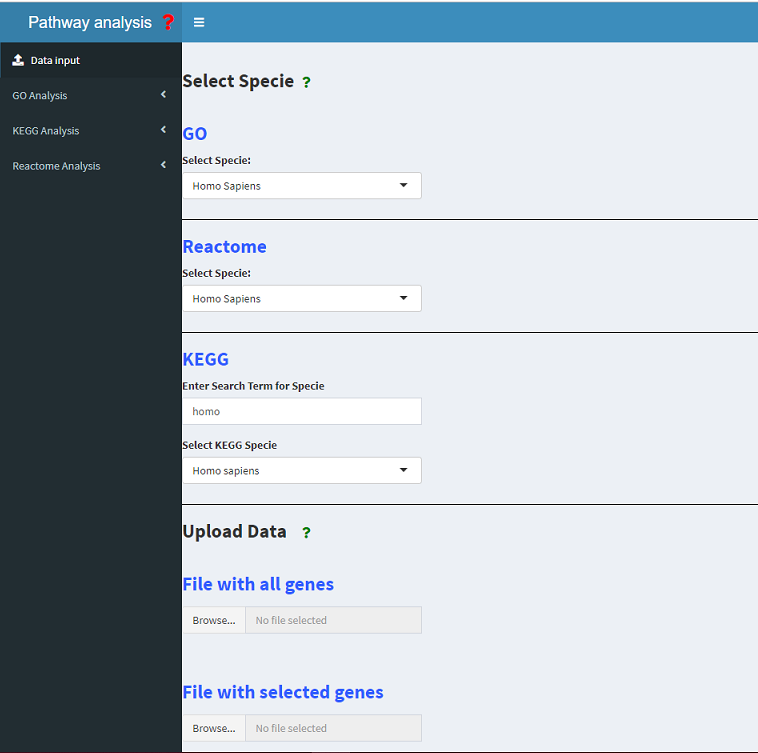
\includegraphics[width=0.9\textwidth]{figures/App_F1.png}
\end{figure}

L'usuari té la possibilitat d'introduir l'arxiu amb tots els gens i els gens seleccionats. Un cop introduïdes les dades es mostra un petit resum del contingut dels arxius.

\begin{figure}[H]
\caption{Resum de les dades pujades}
\centering
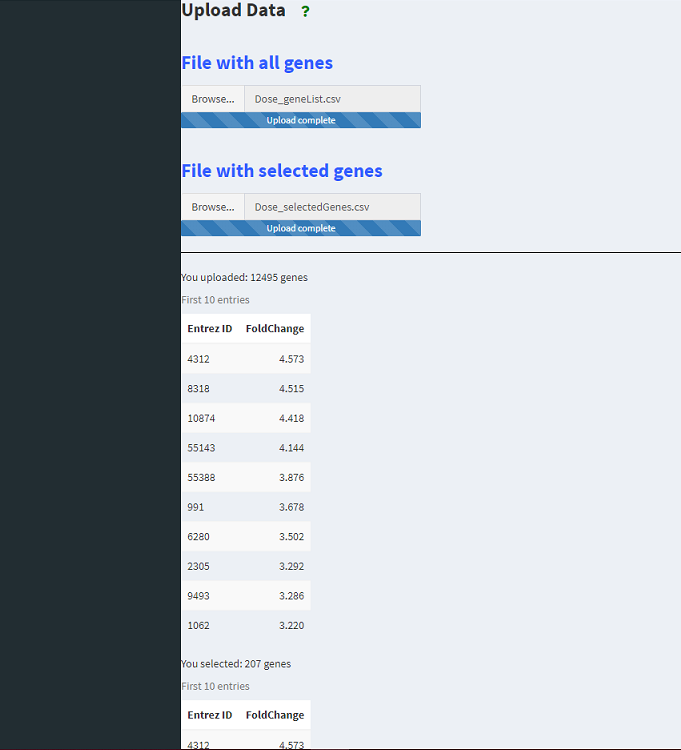
\includegraphics[width=0.9\textwidth]{figures/App_F1b.png}
\end{figure}


L'aplicació està dividida doncs en 4 parts substancials:

\begin{enumerate}
\item Entrada de les dades;
\item Anàlisi \gls{GO};
\item Anàlisi \gls{KEGG};
\item Anàlisi Reactome.
\end{enumerate}


L'aplicació ofereix dos mètodes d'anàlisi: d'una banda es pot fer \gls{ORA} i d'altra banda l'anàlisi \gls{GSEA}. Recordem que l'ORA consisteix a seleccionar els gens diferencialment expressats i basant-se en GO, KEGG o Reactome comprovar si una de les agrupacions de gens suggerides per aquestes bases de dades està sobre o sotraexpressada en els gens seleccionats. Per dur a terme l'ORA l'usuari té l’opció de definir un \textit{cut-off} de Log-Ratio per formar el conjunt dels gens que s'hi utilitzarà (\textit{gene set}). ORA és una bona eina per veure els efectes grans però els efectes petits se li escapen. Els efectes petits derivats dels gens individuals poden acumular-se en un efecte conjunt substancial el qual ORA no serà capaç de detectar. És aquí on GSEA mostra la seva utilitat. 

Els apartats d'anàlisi (\gls{GO}, \gls{KEGG} i Reactome) ofereixen tan representacions comunes com representacions específiques. 

Els anàlisis i representacions en comú són:

\begin{itemize}
\item Taula dels resultats \gls{ORA};
\item Taula dels resultats \gls{GSEA};
\item Gràfic de barres del resultat \gls{ORA};
\item Gràfic de punts del resultat \gls{ORA};
\item El mapa d'enriquement (\gls{Enrichment Map});
\item La xarxa dels gens en categories (Category-gene-network);
\item El gràfic de \gls{GSEA}.
\end{itemize} 

Les anàlisis específics són:

\begin{itemize}
\item GO $\rightarrow$ Gràfic \gls{GO} 
\item KEGG $\rightarrow$ Rutes de la base de dades \gls{KEGG}
\item Reactome $\rightarrow$ Rutes de la base de dades Reactome
\end{itemize}

\begin{figure}[H]
\centering
\begin{tabular}{ccc}
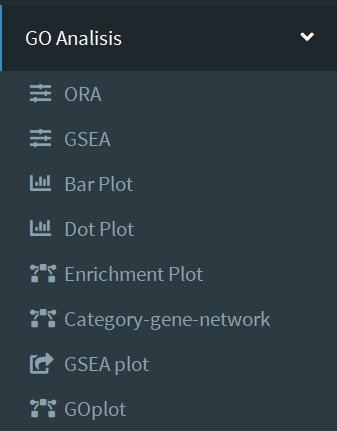
\includegraphics[width=45mm]{figures/App_F2_Items_GO.png} & 
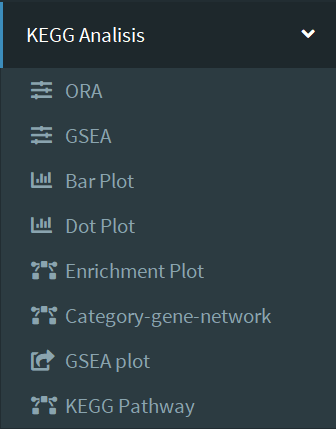
\includegraphics[width=45mm]{figures/App_F3_Items_KEGG.png} &
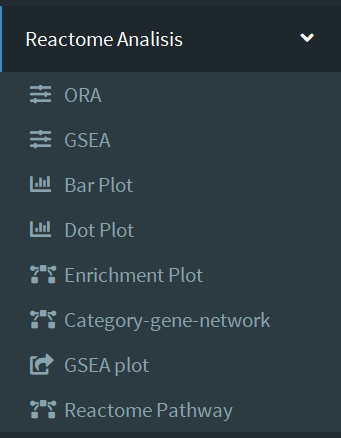
\includegraphics[width=45mm]{figures/App_F4_Items_RA.png} \\
(a) GO & (b) KEGG & (c) Reactome \\
\end{tabular}
\caption{Els elements de les seccions d'anàlisi}
\end{figure}


\label{sec:ACom}

\section{\gls{ORA}}

\subsection{\gls{GO}}

Per realitzar l'anàlisi \gls{ORA} per a termes \gls{GO} s'utilitza la funció \helvetica{enrichGO} del paquet \helvetica{clusterPrifiler}.

He implementat els valors per defecte amb la possibilitat per a l’usuari d'elegir entre:

\begin{itemize}
\item \underline{Ontologies \gls{GO}} 
\begin{itemize}
\item Molecular function, Biological proces, Cellular Components;
\end{itemize}
\item \underline{Nivell de significació basant-se en els valors de P ajustats}
\begin{itemize}
\item 0.1, 0.05, 0.01, 0.001;
\end{itemize}
\item \underline{Mètode d'ajustament}
\begin{itemize}
\item Holm; Hochberg; Hommel; Bonferroni; BH; BY; FDR; None.
\end{itemize}
\end{itemize}

\begin{figure}[h!]
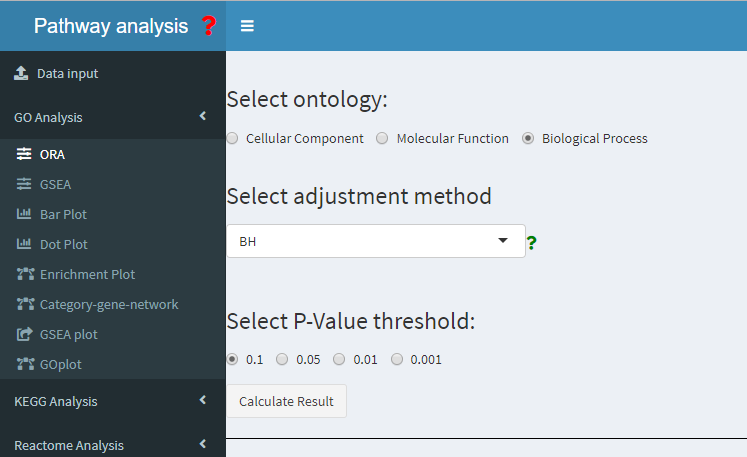
\includegraphics[width=0.9\textwidth]{figures/App_F5_Items_GO_ORA.png}
\caption{Especificació d'\gls{ORA} dels termes \gls{GO}}
\end{figure}
L'execució de la funció és un procès temporalment costós. Per aquest motiu he afegit el botó d'acció, en lloc de deixar la funció reactiva. D'aquesta manera l'usuari ha de fer una decisió conscient de repetir l'anàlisi amb altres valors.

Prement el botó apareix la taula i el botó nou mitjançant el qual l'usuari pot descarregar els resultats en format .csv. He formatejat la taula amb els paquets \helvetica{knitr}, \helvetica{kableExtra}, \helvetica{formattable} i \helvetica{dplyr}. Amb els dos últims he afegit les barres de color pel nombre dels gens diferencialment expressats del terme específic de \gls{GO} i la gradació de color del verd fins al vermell pels valors dels més petits fins els més grans. 

\begin{figure}[h!]
\centering
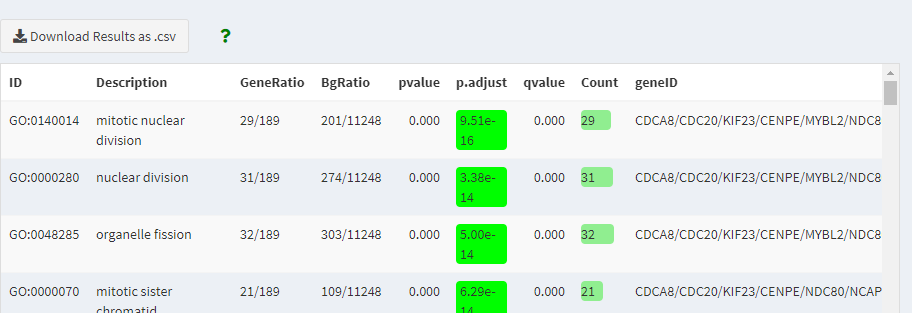
\includegraphics[width=0.9\textwidth]{figures/App_F6_Items_GO_ORA_Table.png} 
\caption{El resultat d'anàlisi \gls{ORA}. \gls{GO}.}
\end{figure}


\subsection{\gls{KEGG}}

Per l'ORA de base de dades \gls{KEGG} he utilitzat la funció \helvetica{enrichKEGG()} del paquet \helvetica{clusterProfiler}. 



\begin{figure}[H]
\centering
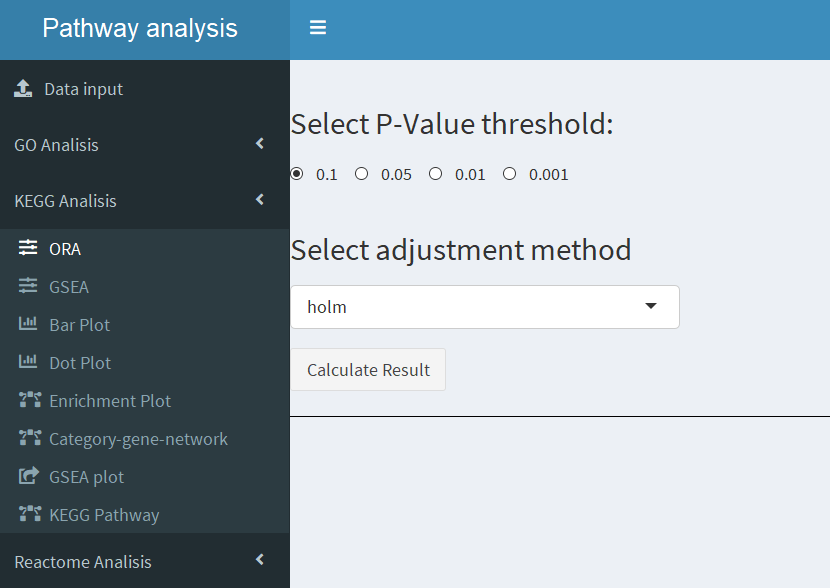
\includegraphics[width=0.9\textwidth]{figures/App_F7_Items_KEGG_ORA.png} 
\caption{Configuració d'anàlisi \gls{KEGG}}
\end{figure}



Una vegada introduïts els paràmetres i premut el botó \textbf{Calculate} apareix el botó \textbf{Download .csv} i la taula previsualitzada. Els camps de la taula són els mateixos com en l'anàlisi dels termes GO.
\begin{figure}[H]
\centering
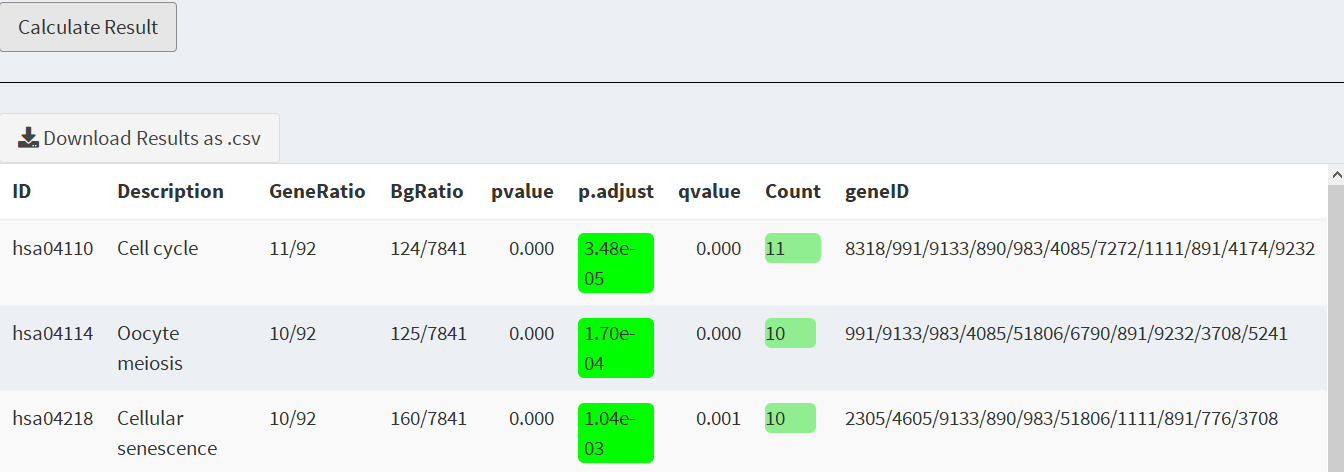
\includegraphics[width=0.9\textwidth]{figures/App_F9_Items_KEGG_ORA_Table.png} 
\caption{El resultat de l'anàlisi \gls{ORA}. \gls{KEGG}.}
\end{figure}

\subsection{Reactome}
En el cas de Reactome el procediment és similar. La funció usada és \helvetica{enrichPathway()} del paquet \helvetica{ReactomePA}:


\begin{figure}[H]
\centering
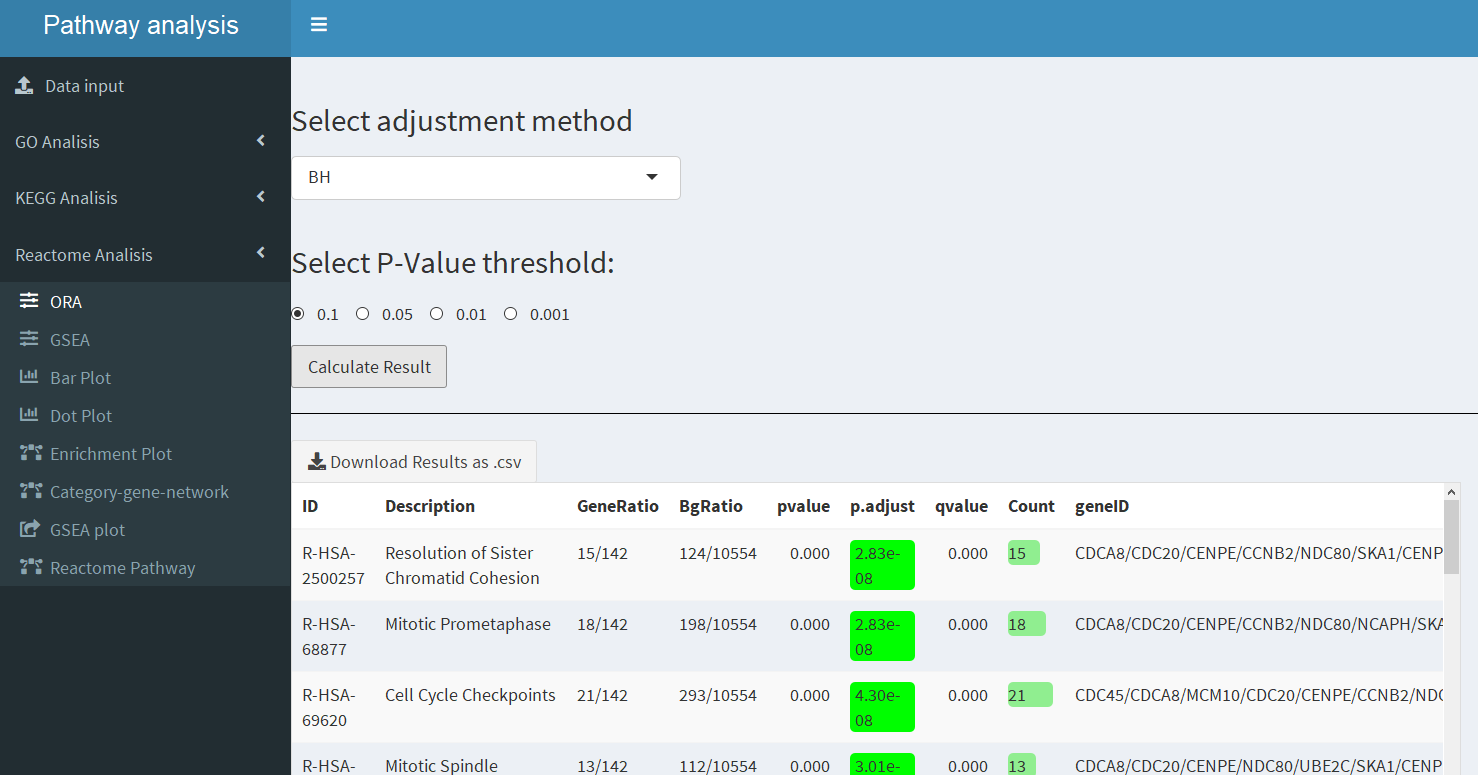
\includegraphics[width=0.9\textwidth]{figures/App_F10_Items_Reactome_ORA.png} 
\caption{El resultat d'anàlisi \gls{ORA}. Reactome.}
\end{figure}

\section{\gls{GSEA}}
\subsection{\gls{GO}}
El mètode \gls{GSEA} per a termes \gls{GO} es calcula amb la funció \helvetica{gseGO()} del paquet \helvetica{clusterProfiler}. 

L'usuari pot elegir l'ontologia \gls{GO}, el \textit{cut-off} del valor P i el mètode d'ajustament.
\begin{figure}[H]
\centering
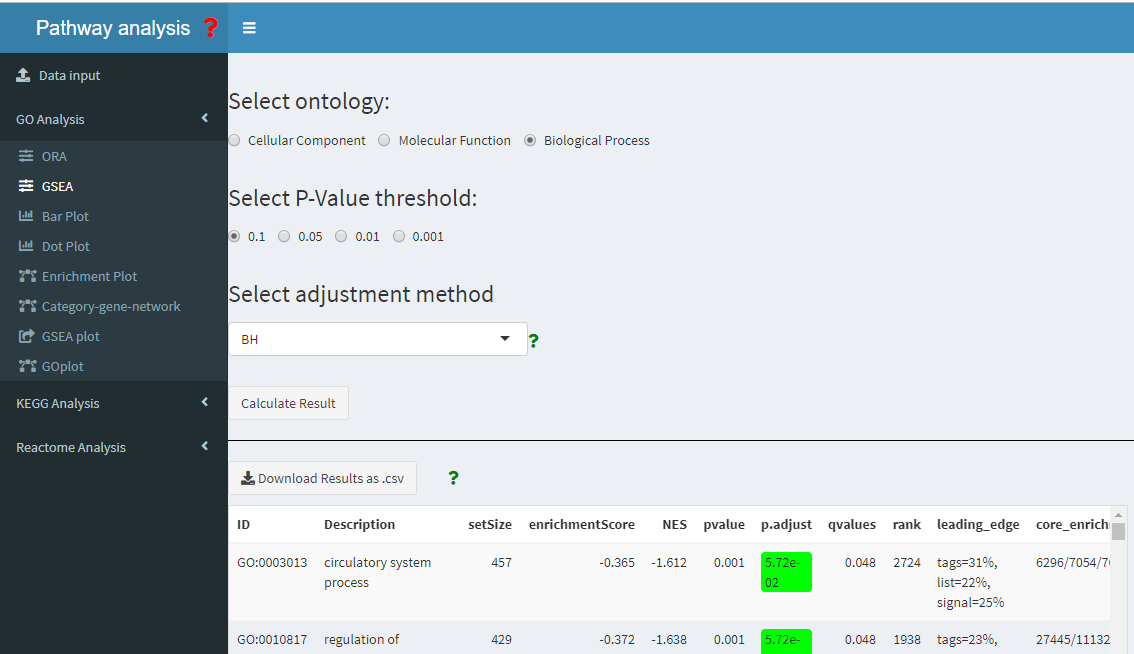
\includegraphics[width=0.9\textwidth]{figures/App_F11_Items_GO_GSEA.png} 
\caption{El resultat de l'anàlisi \gls{GSEA}. \gls{GO}.}
\end{figure}


\subsection{\gls{KEGG}}
De la mateixa manera es calcula \gls{GSEA} amb la funció \helvetica{gseKEGG()} del paquet \helvetica{clusterProfiler}:

\begin{figure}[H]
\centering
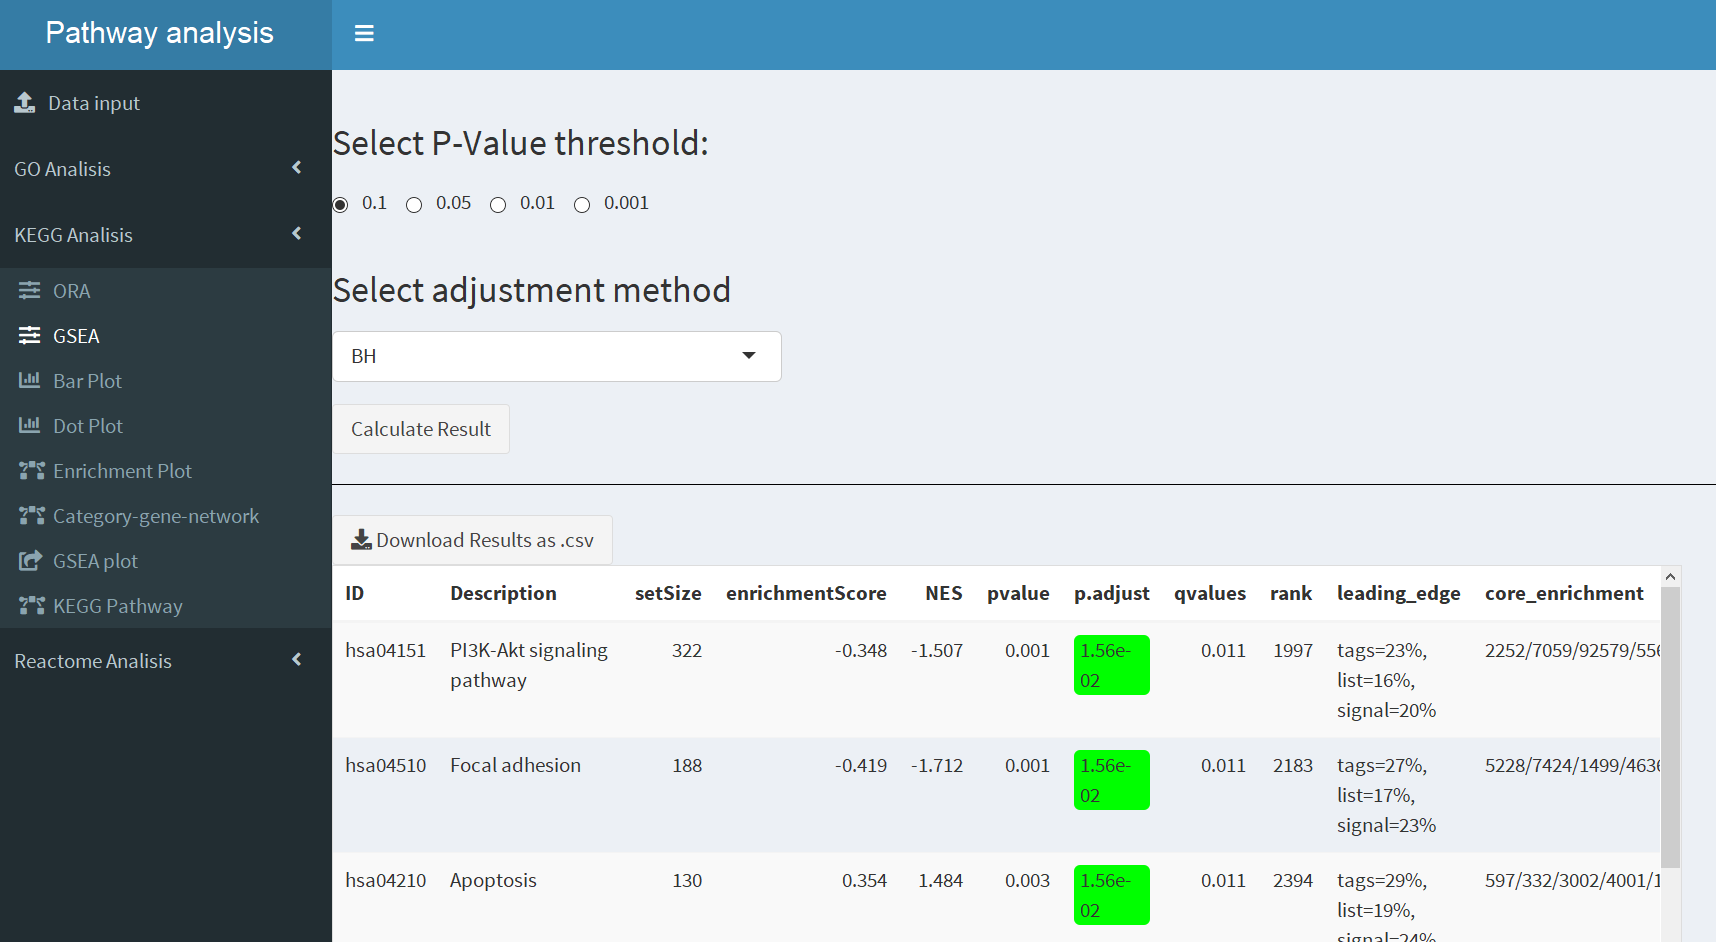
\includegraphics[width=0.9\textwidth]{figures/App_F12_Items_KEGG_GSEA.png} 
\caption{El resultat de l'anàlisi \gls{GSEA}. \gls{KEGG}.}
\end{figure}

\subsection{Reactome}
Per completar l'anàlisi l'usuari pot calcular \gls{GSEA} per a base de dades Reactome. Com als altres casos utilitzo el paquet \helvetica{clusterProfiler} i específicament la funció \helvetica{gsePathway()}

\begin{figure}[H]
\centering
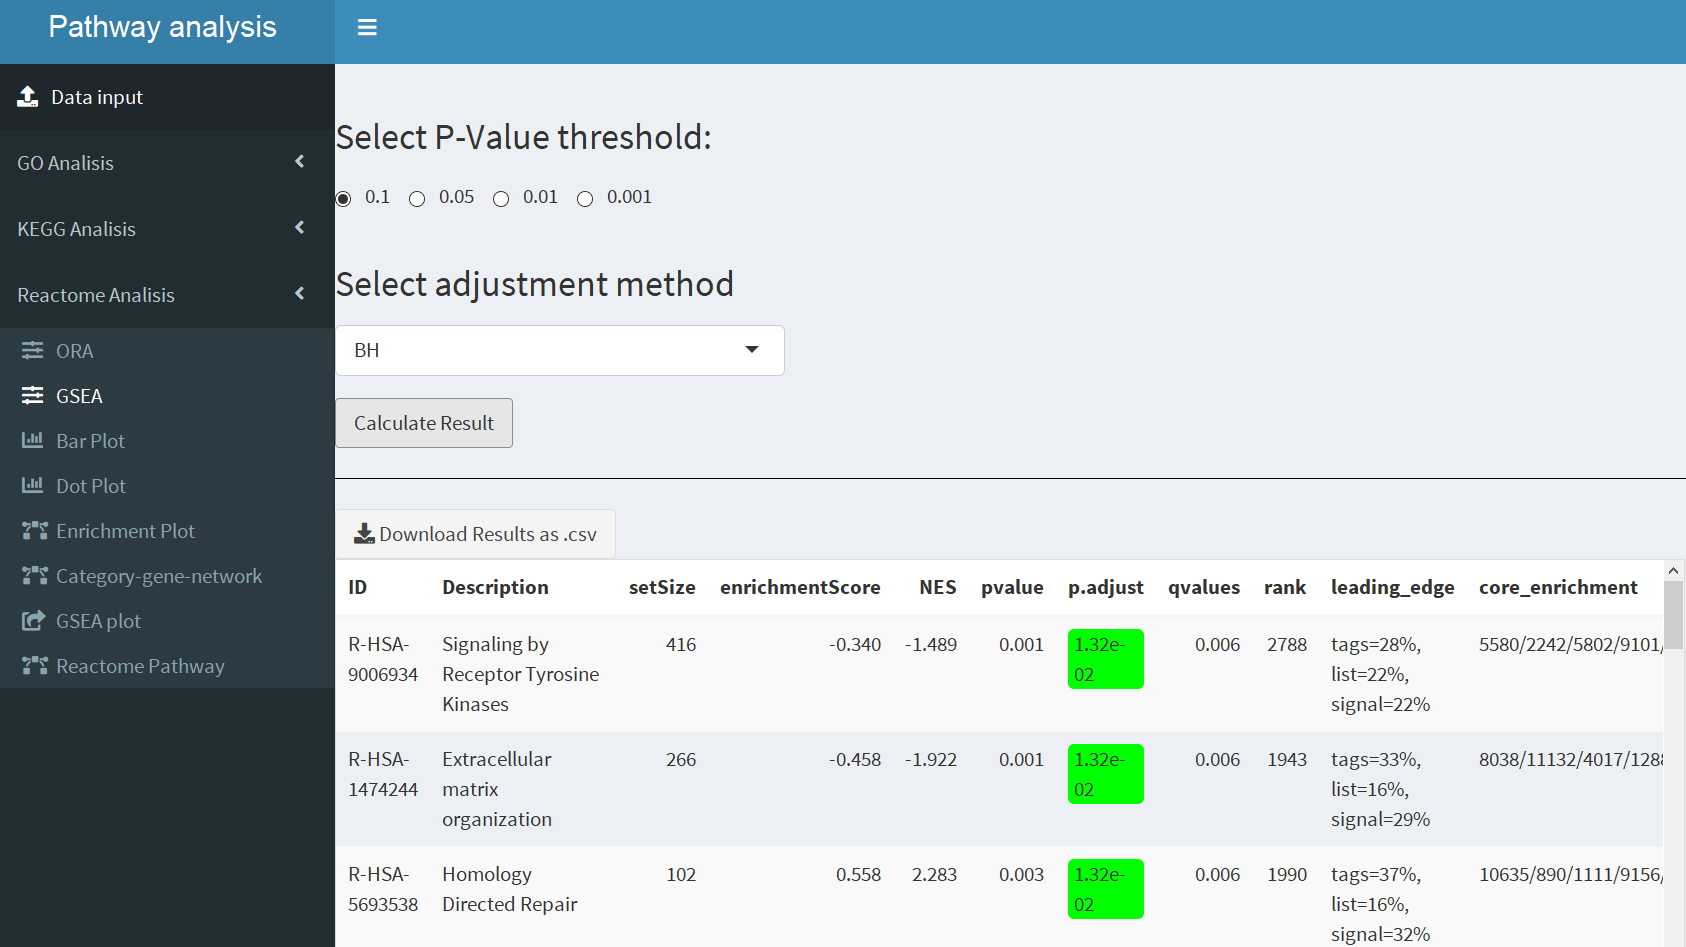
\includegraphics[width=0.9\textwidth]{figures/App_F13_Items_RA_GSEA.png} 
\caption{El resultat d'anàlisi \gls{GSEA}. Reactome.}
\end{figure}

\section{Visualització i l'anàlisi topològic}

\subsection{\gls{Bar-Plot}s}
Els resultats de \helvetica{enrichGO}, \helvetica{enrichKEGG} i \helvetica{enrichPathway} es poden visualitzar amb el gràfic de barres. L'usuari pot elegir el nombre de categories visualitzades entre 2 i 30. Es dona l'opció per descarregar el gràfic en format .png.

\begin{figure}[H]
\centering
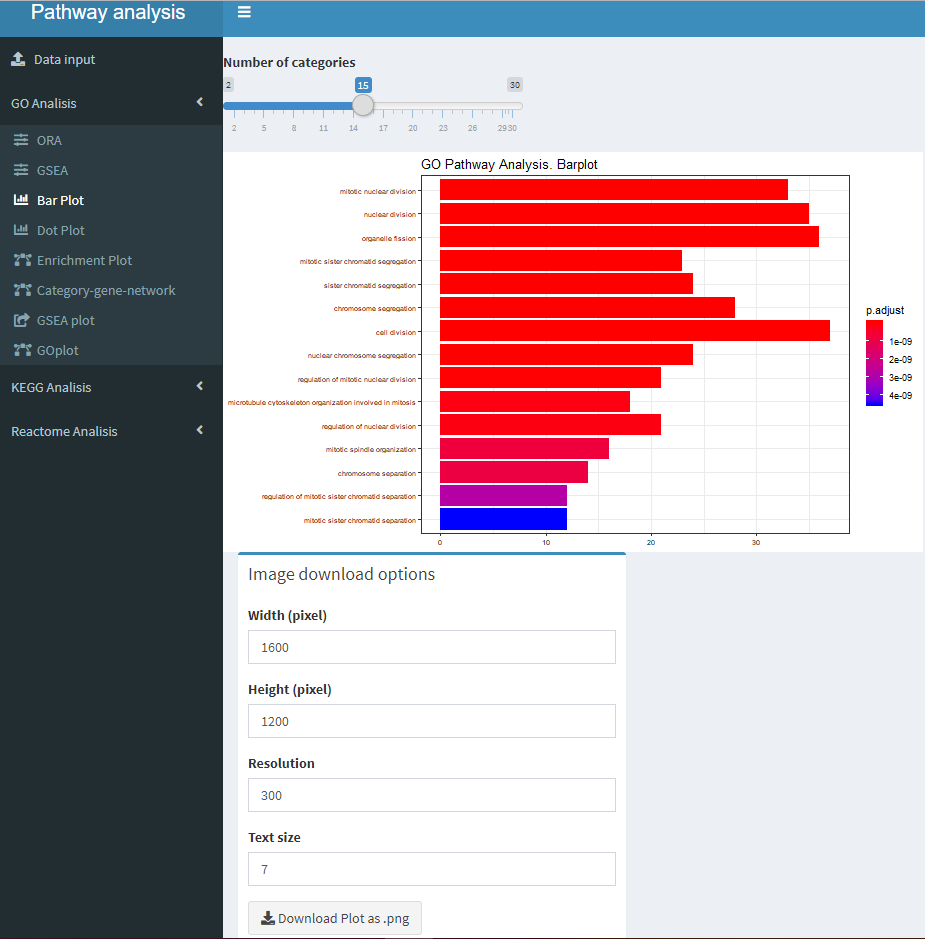
\includegraphics[width=0.9\textwidth]{figures/App_F14_Items_GO_BarPlot.png} 
\caption{\gls{Bar-Plot}. \gls{GO}.}
\end{figure}

\subsection{\gls{Dot-Plot}s}

El \textit{\gls{Dot-Plot}} visualitza addicionalment el \textit{gen ratio}. També aquí l'usuari pot seleccionar el nombre de categories.


\begin{figure}[H]
\centering
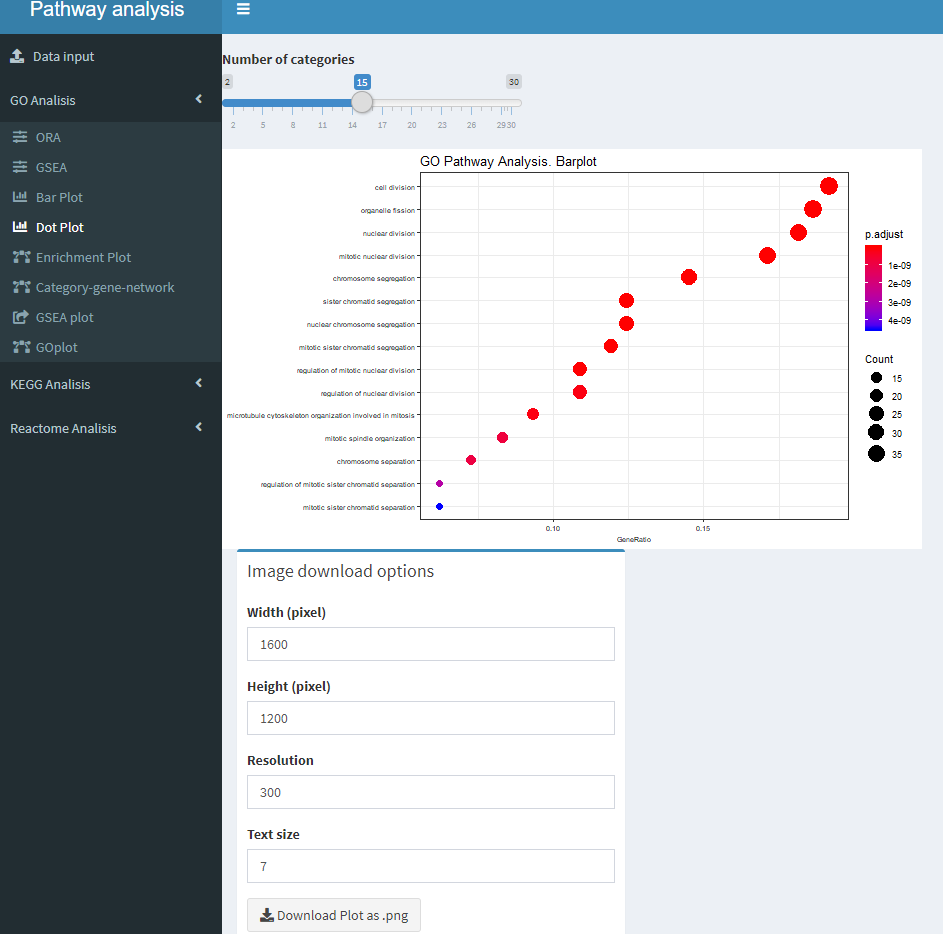
\includegraphics[width=0.9\textwidth]{figures/App_F15_Items_GO_DotPlot.png} 
\caption{\gls{Dot-Plot}. GO.}
\end{figure}

\subsection{\gls{Enrichment Map}s}

\begin{figure}[H]
\centering
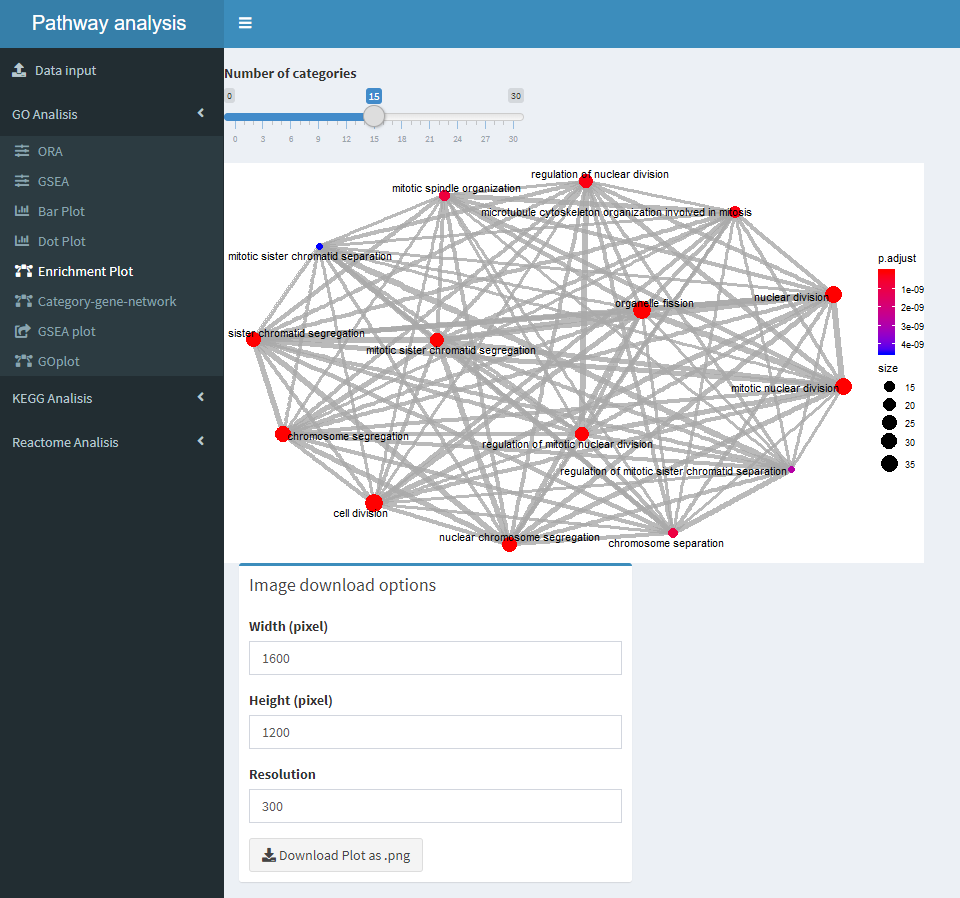
\includegraphics[width=0.9\textwidth]{figures/App_F16_Items_GO_Emap.png} 
\caption{\gls{Enrichment Map}. GO.}
\end{figure}

\subsection{Category-Gene-Network Plot}

\begin{figure}[H]
\centering
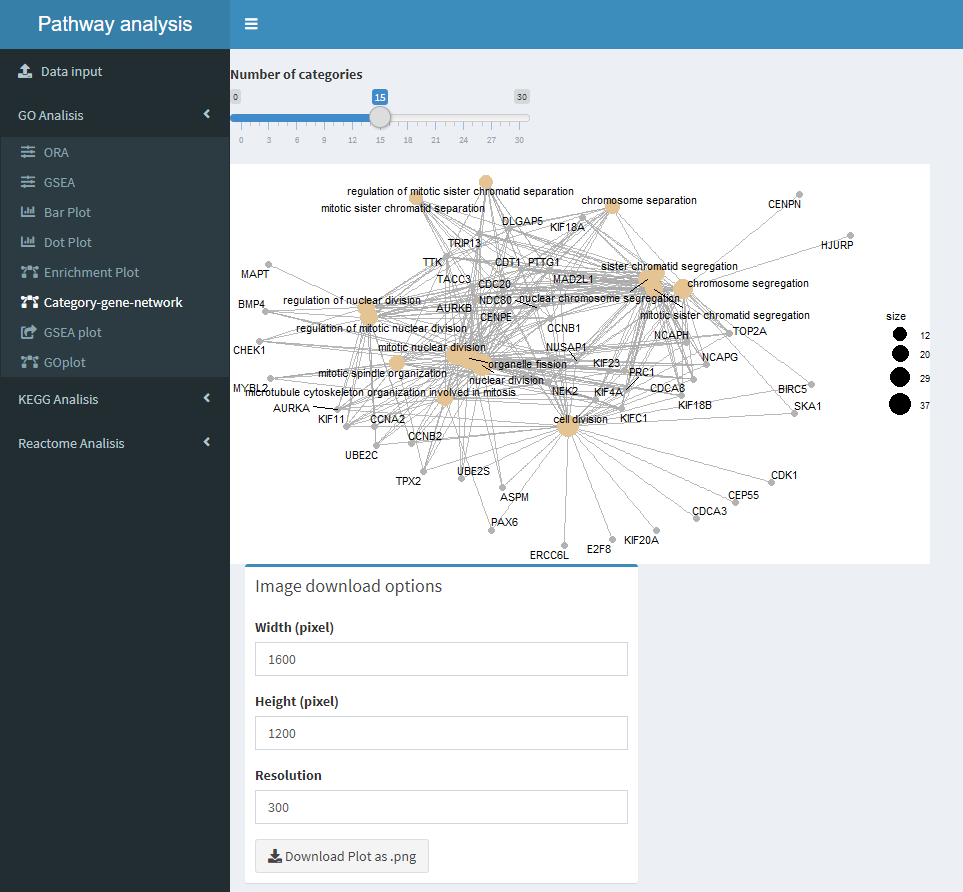
\includegraphics[width=0.9\textwidth]{figures/App_F17_Items_GO_CnetPlot.png} 
\caption{Category-Gene-Network Plot. GO.}
\end{figure}

\subsection{\gls{GSEA} Plot}
L'usuari pot visualitzar una de les categories disponibles via \textit{dropdown list}. El llistat inclou totes les rutes generades durant l'anàlisi GSEA en els apartats \textit{Go Analysis}$\rightarrow$\textit{GSEA}; \textit{KEGG}$\rightarrow$\textit{GSEA}
\begin{figure}[H]
\centering
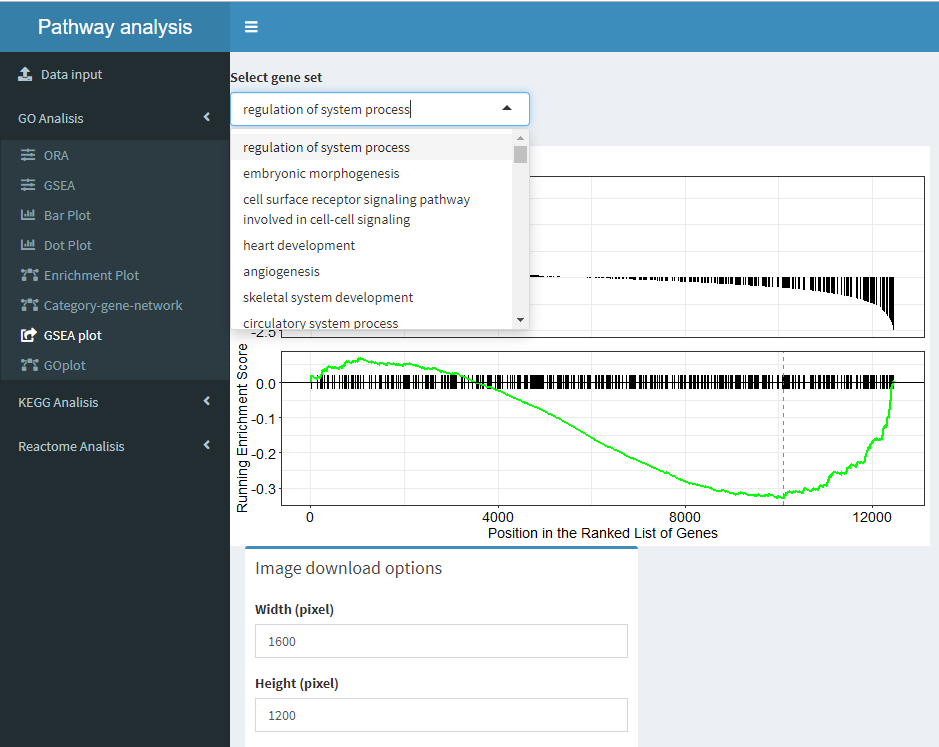
\includegraphics[width=0.9\textwidth]{figures/App_F18_Items_GO_GSEA_Plot.png} 
\caption{\gls{GSEA} Plot. \gls{GO}.}
\end{figure}


\subsection{GO Plot}

\begin{figure}[H]
\centering
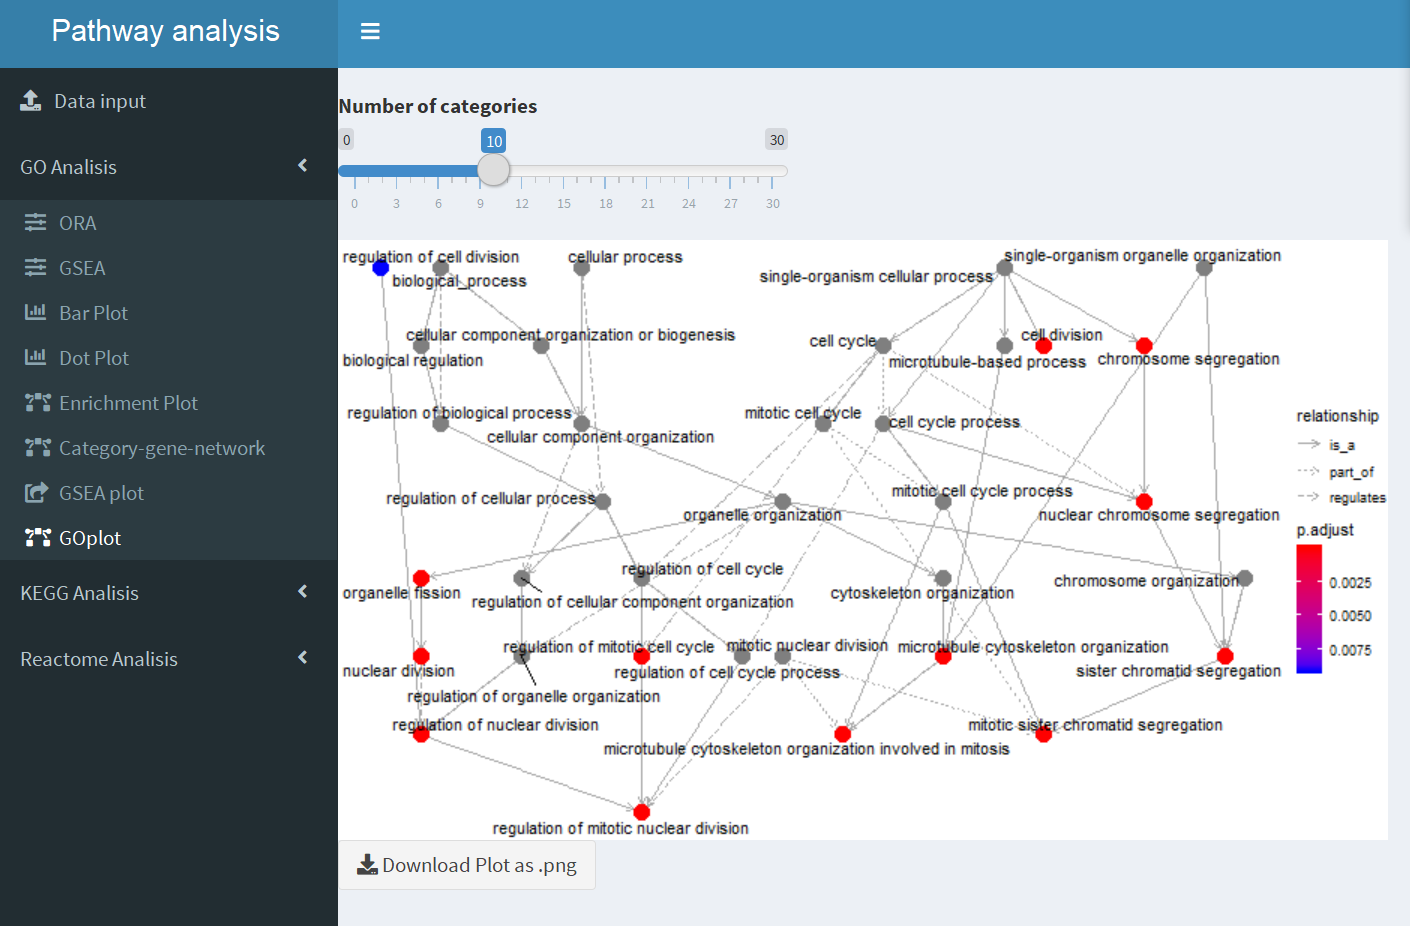
\includegraphics[width=0.9\textwidth]{figures/App_F19_Items_GO_GOPlot.png} 
\caption{\gls{GO} Plot}
\end{figure}

\subsection{\gls{KEGG} Pathway}


\begin{figure}[H]
\centering
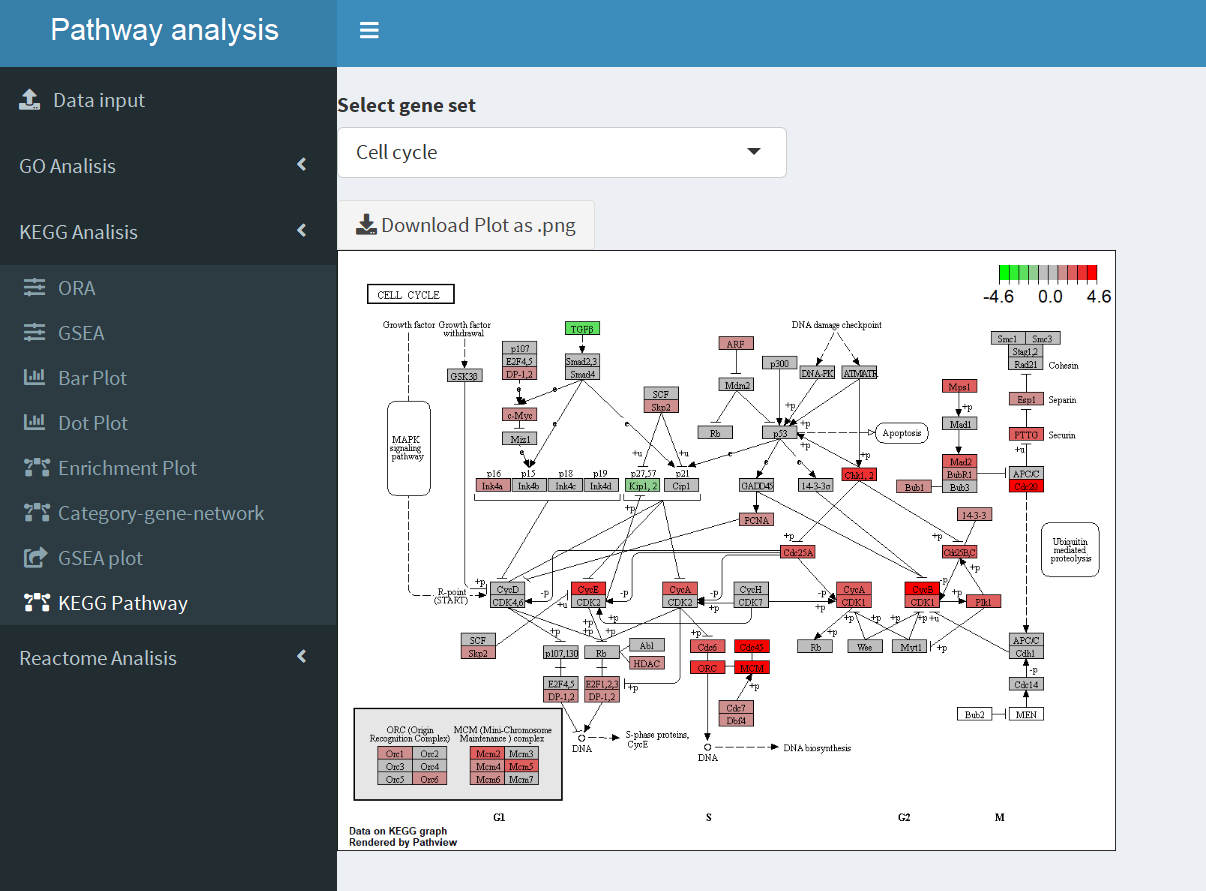
\includegraphics[width=0.9\textwidth]{figures/App_F20_Items_KEGG_KEGGPathway.png} 
\caption{\gls{KEGG} pathway}
\end{figure}

\subsection{Reactome Pathway}

\begin{figure}[H]
\centering
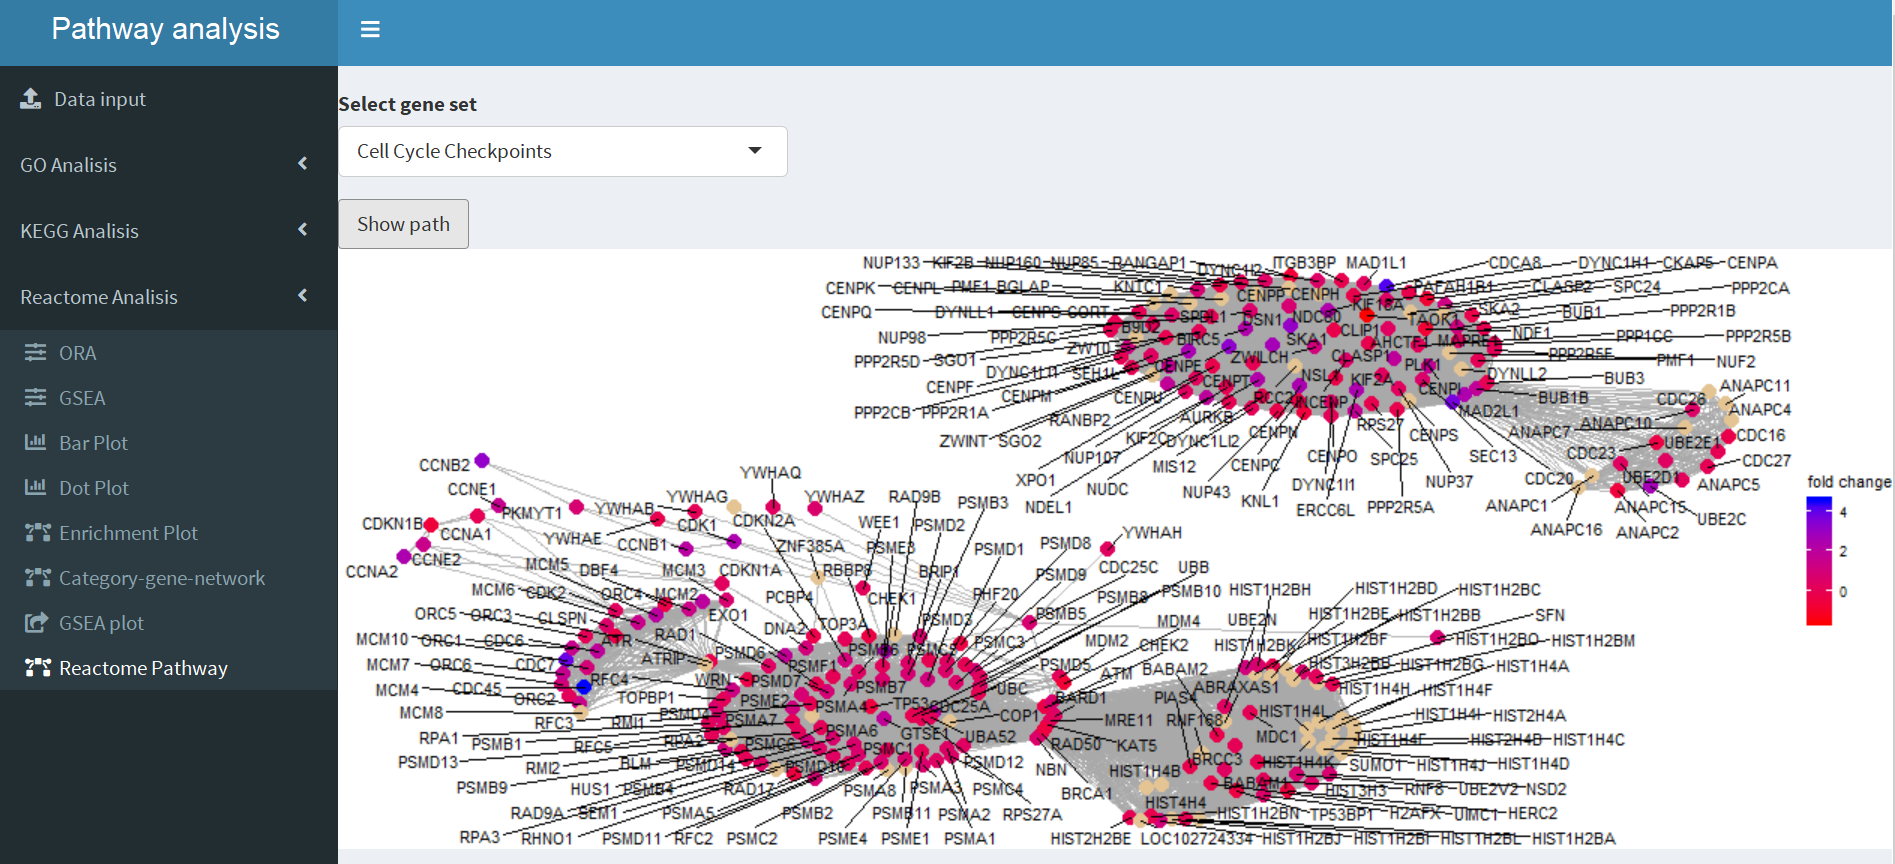
\includegraphics[width=0.9\textwidth]{figures/App_F21_Items_RA_RAPathway.png} 
\caption{Reactome pathway}
\end{figure}


\section{Manual i ajudes del programa}

Per facilitar l'ús de l’aplicació he pensat com es podria fer de manera el més intuïtiva possible. Primer cal destacar que com a llengua de manual he elegit l’anglès per poder fer l'ús de l'aplicació el més inclusiu possible. Segon, l'usuari pot accedir tant al manual com a l'ajuda, que es guarden en arxius .Md separats. Per accedir al manual l'usuari ha de clicar al símbol d’interrogació a prop del títol \textbf{Pathway analysis}:
\begin{figure}[H]
\centering
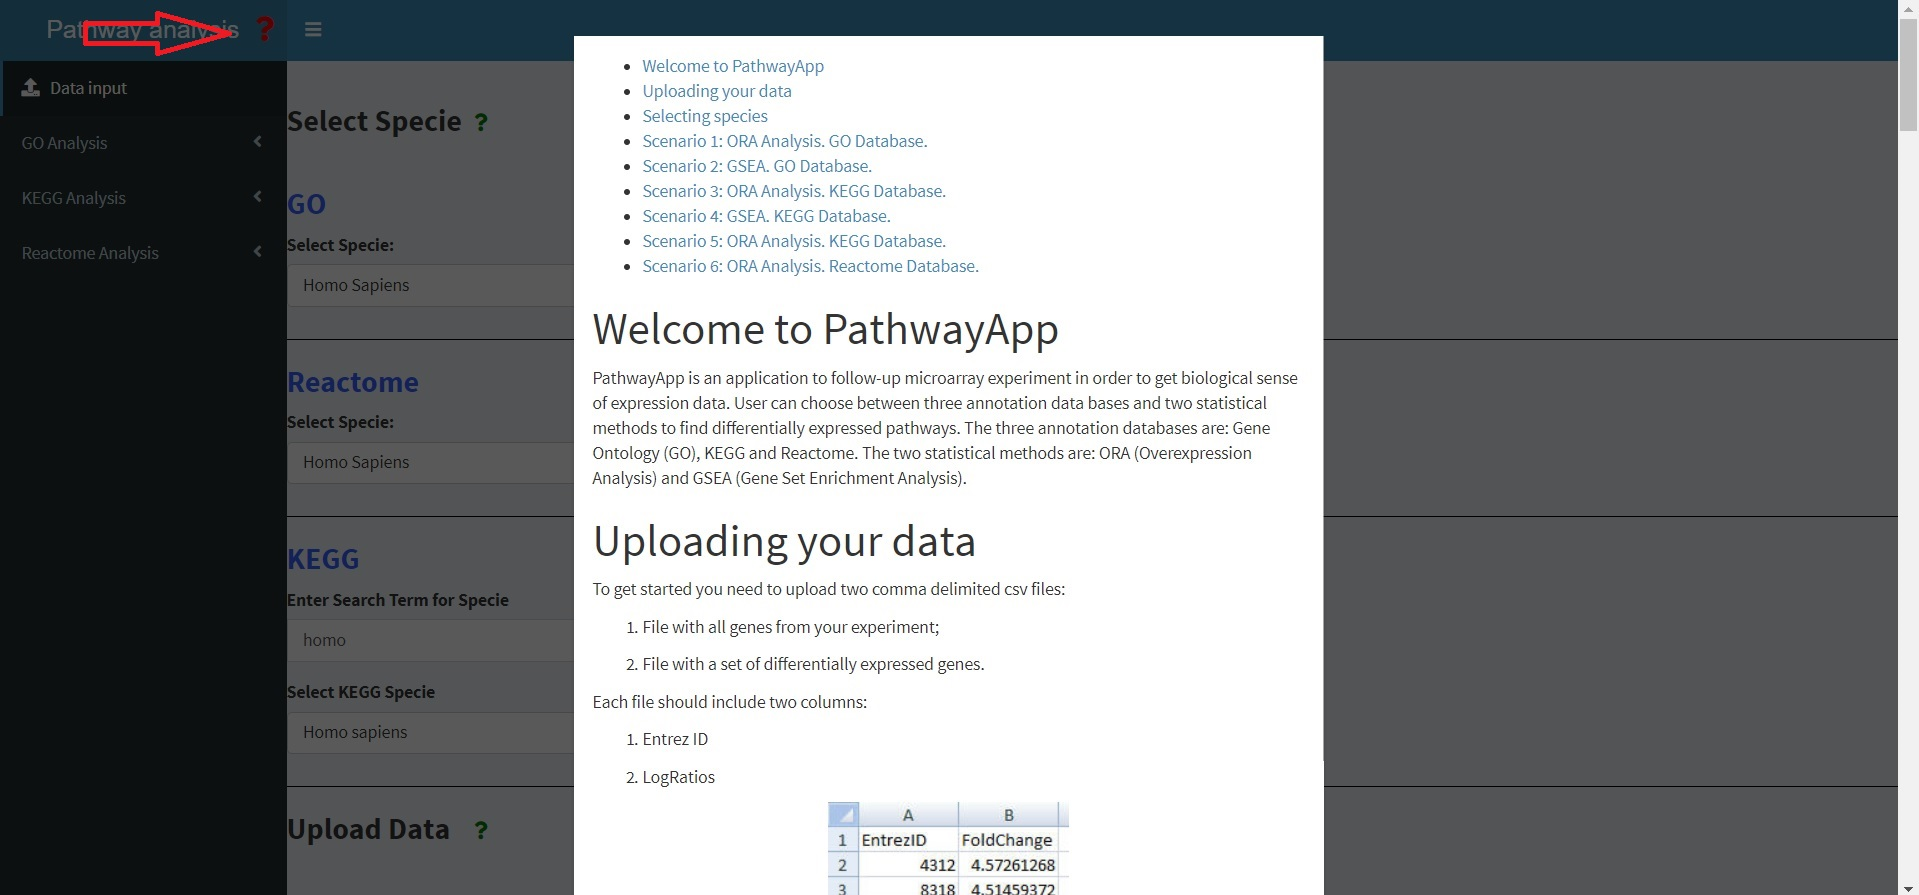
\includegraphics[width=1\textwidth]{figures/Manual.jpg} 
\caption{Manual per a aplicació}
\end{figure}

Com es veu hi ha apartats diferents. Depenent dels objectius de l'usuari, aquest pot seleccionar l'apartat que més li interessi. Així, si l'usuari vol fer l'anàlisi \gls{ORA} amb l'anotació KEGG pot navegar en la secció \textbf{Scenario 3: \gls{ORA} Analysis.\gls{KEGG} Database}. 

\begin{figure}[H]
\centering
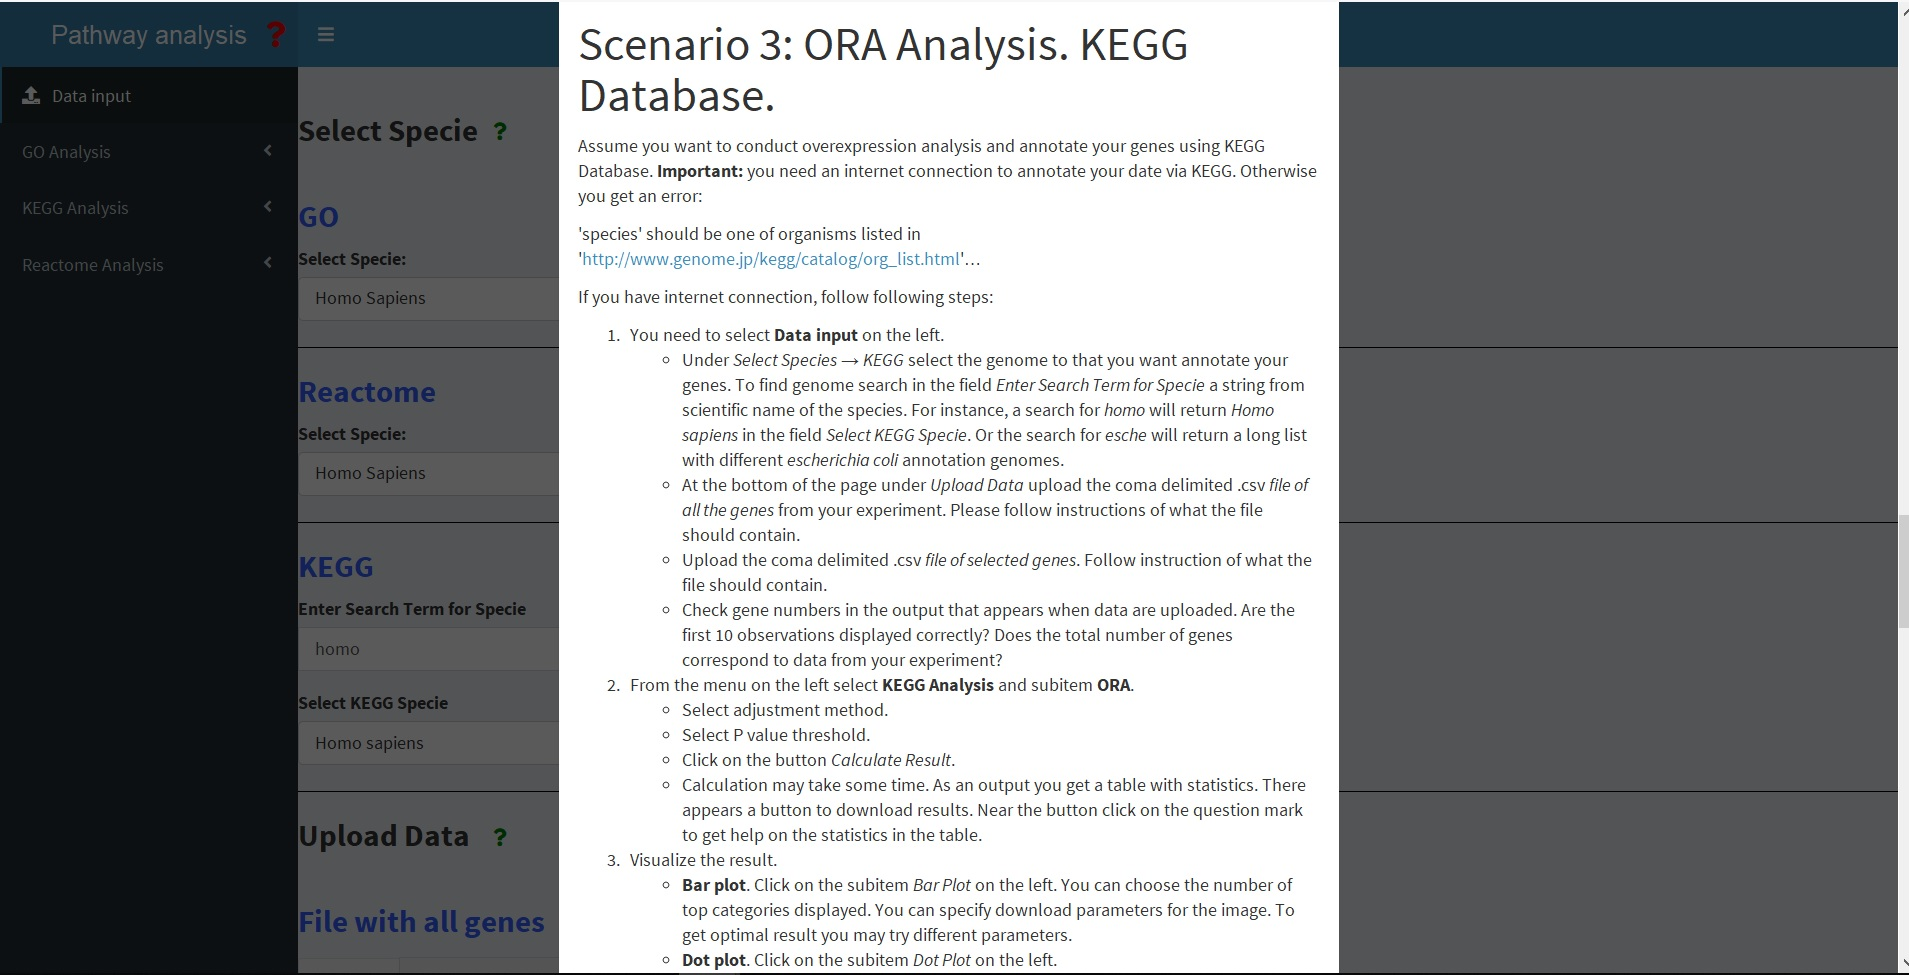
\includegraphics[width=1\textwidth]{figures/Manual2.jpg} 
\caption{Manual per a l'anàlisi \gls{ORA} amb l'anotació \gls{KEGG}}
\end{figure}


També, l'usuari pot accedir a l'ajuda clicant els símbols d'interrogació distribuïts per l’aplicació en els llocs que penso que poden generar dubtes. 

Per fer-ho possible s'utilitza el paquet \helvetica{shinyhelper} que s'instal·la en executar la funció \helvetica{runPathwayApp()}.

\begin{figure}[H]
\centering
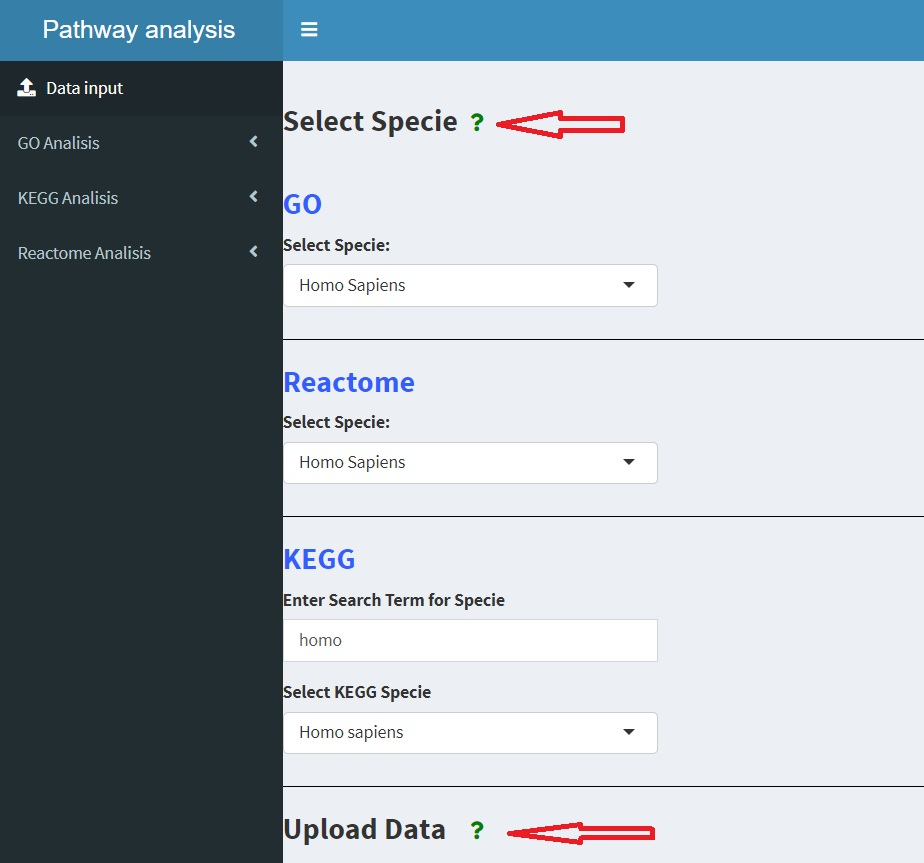
\includegraphics[width=0.7\textwidth]{figures/Help_Data_Input.jpg} 
\caption{Senyals d'ajuda}
\end{figure}

El clic en aquests senyals fa que aparegui una finestreta amb la informació d'ajuda.

Aquí hi ha informació de l'apartat \textbf{Data Input}:

\begin{figure}[H]
\centering
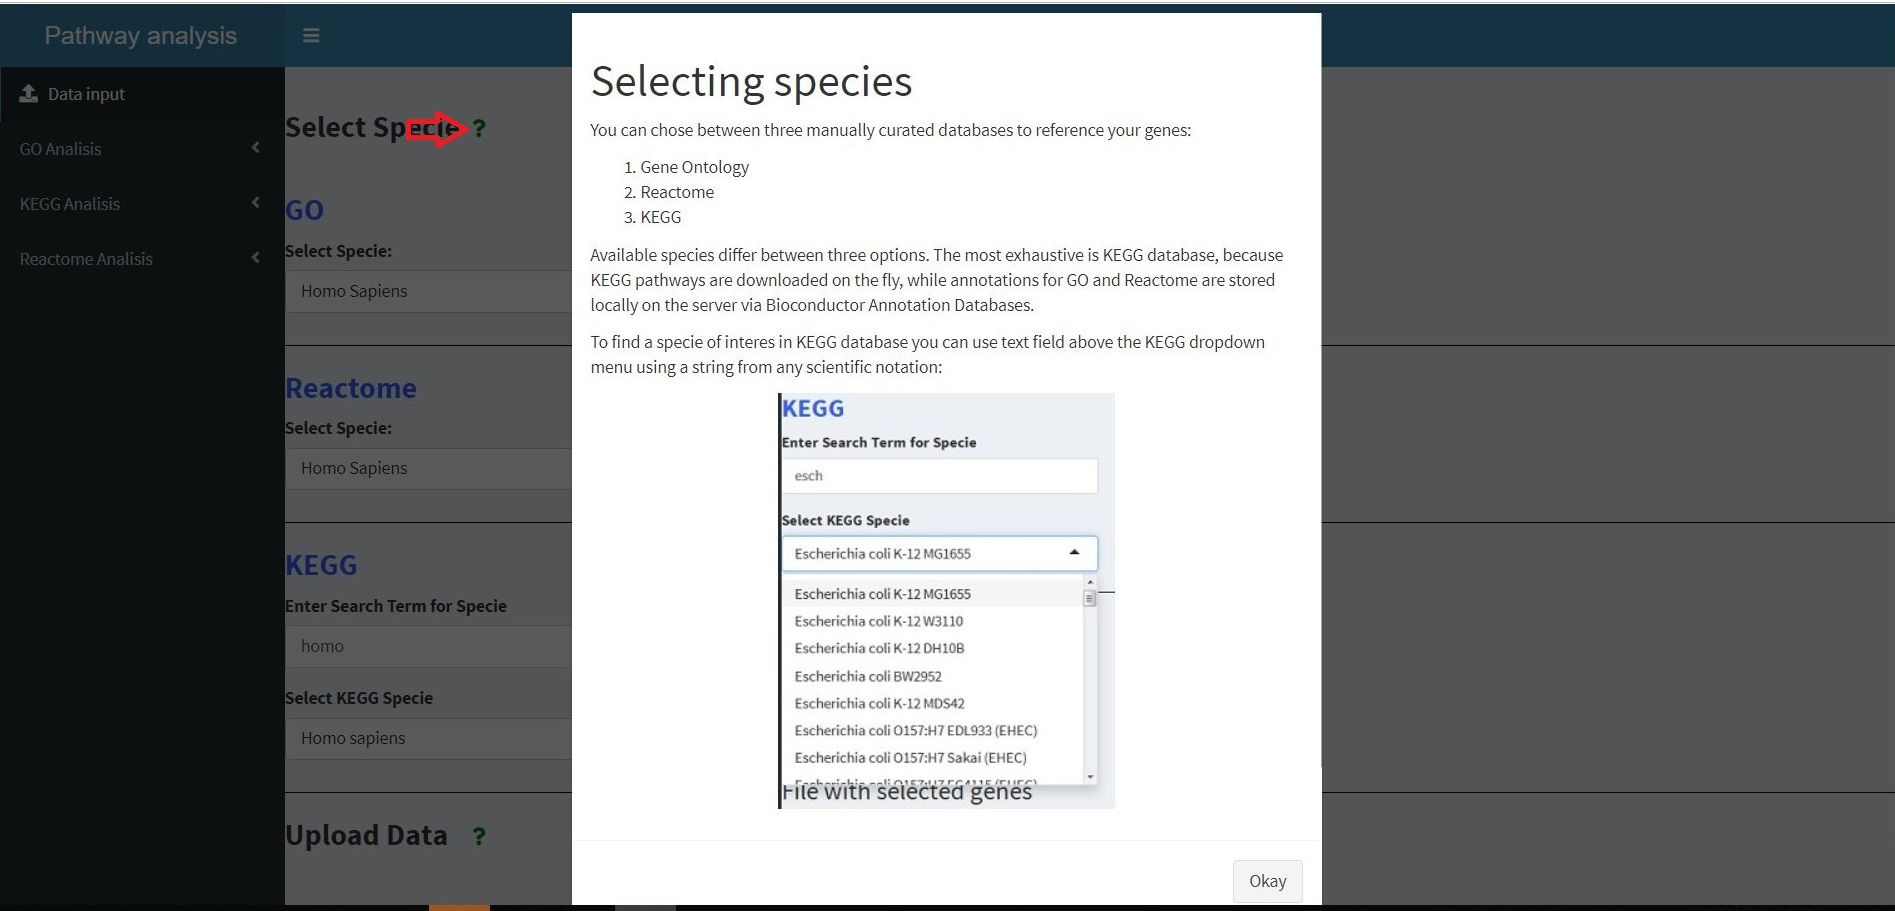
\includegraphics[width=0.9\textwidth]{figures/Help_Specie.jpg} 
\caption{Ajuda per a l'elecció de l'espècie}
\end{figure}

\begin{figure}[H]
\centering
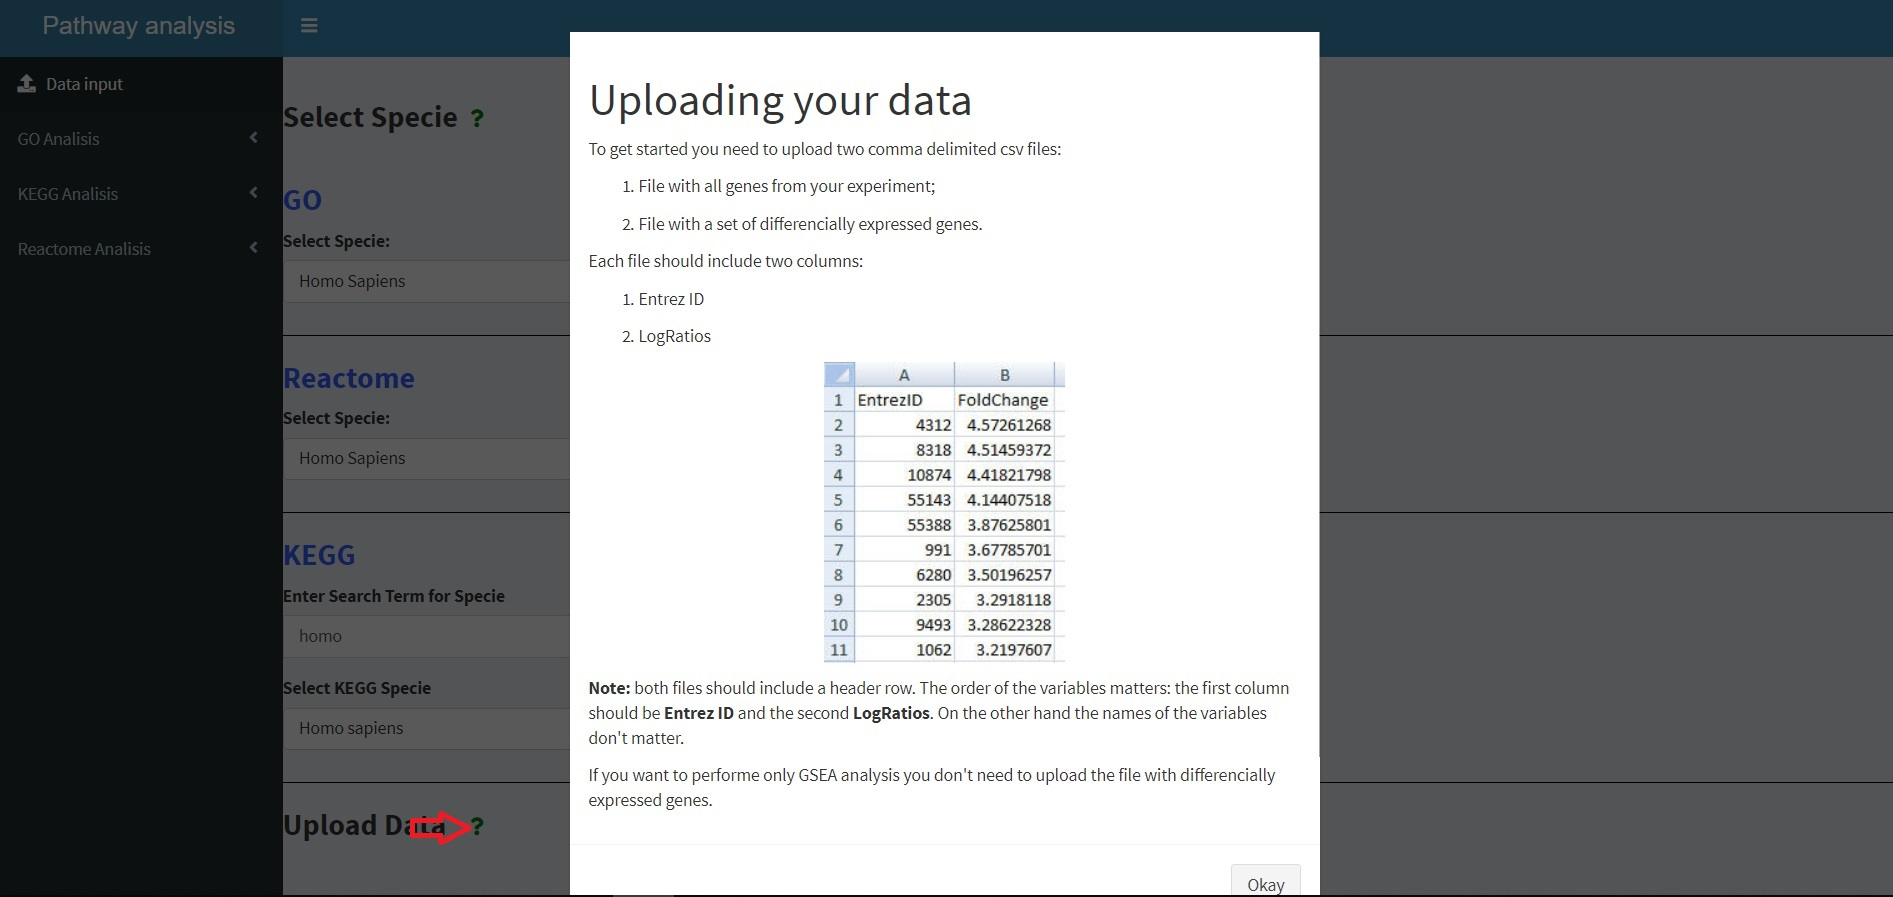
\includegraphics[width=0.9\textwidth]{figures/Help_Upload_Data.jpg} 
\caption{Ajuda per pujar les dades}
\end{figure}

Les informacions per a l'apartat \gls{ORA} són les següents:

\begin{figure}[H]
\centering
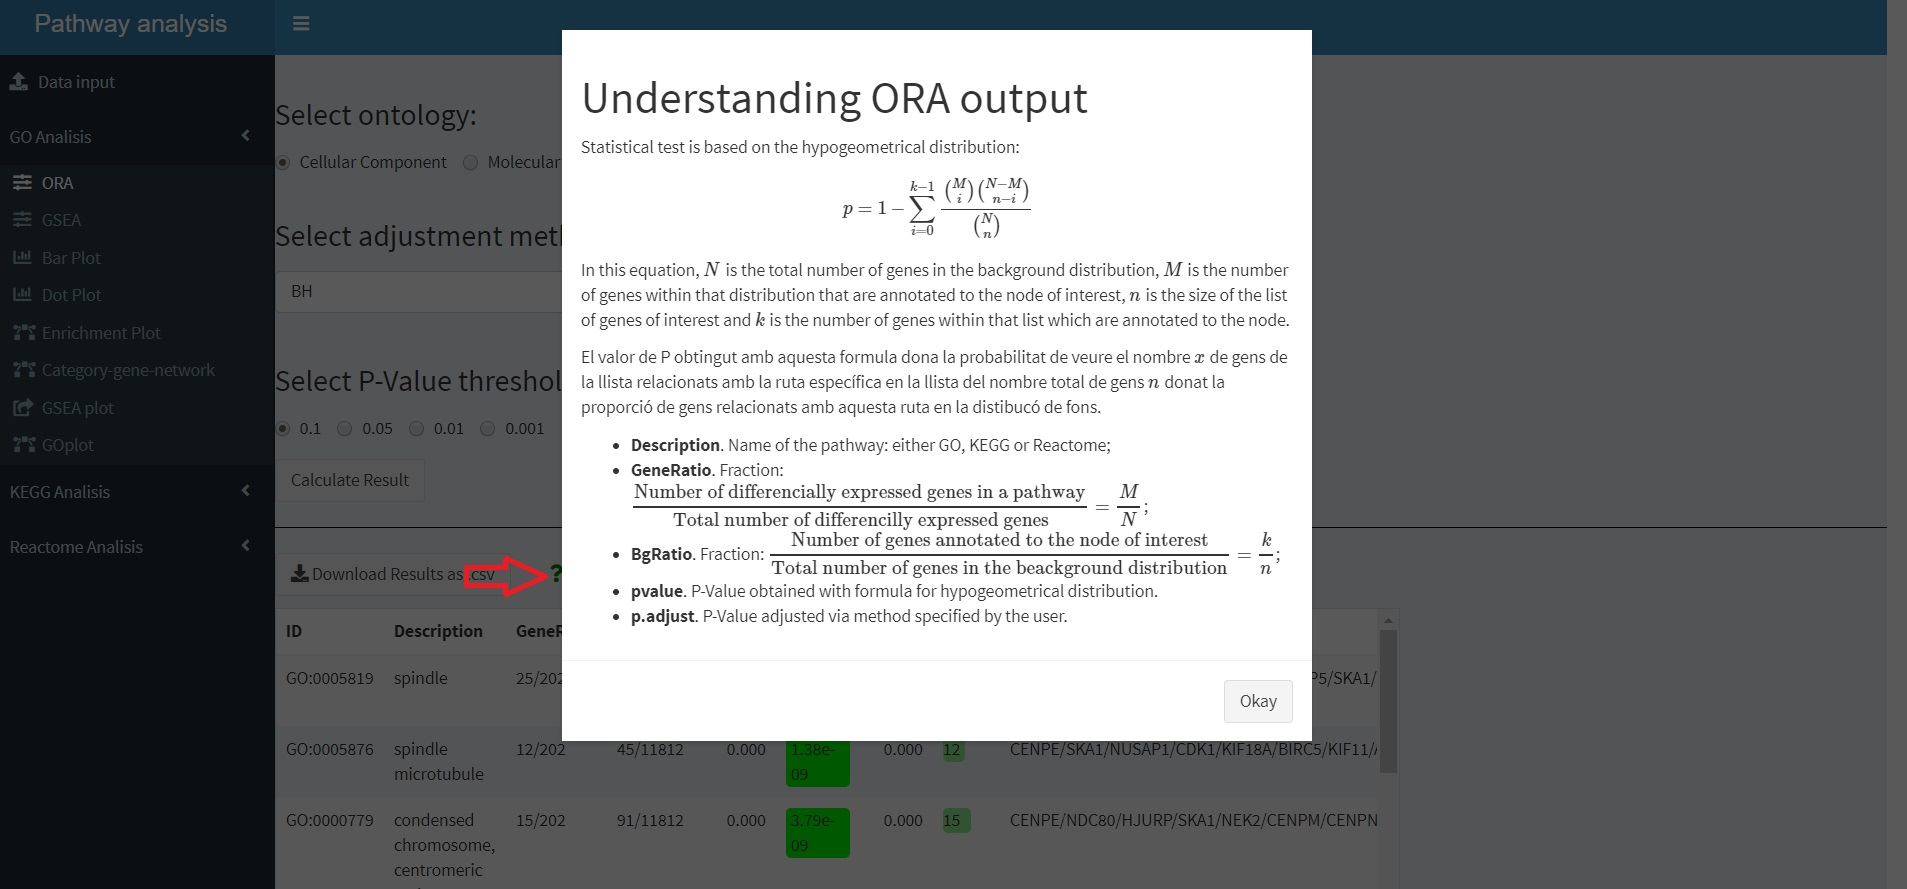
\includegraphics[width=0.9\textwidth]{figures/Help_ORA_output.jpg} 
\caption{Infromació per la interpretació d'anàlisi \gls{ORA}}
\end{figure}
Aquí cal destacar que les fórmules, depenent de l'ordinador, no apareixen degudament en el RStudio Browser. Sí que apareixen bé quan l'aplicació s'obre via l’internet browser. L'usuari ha de tenir connexió amb internet perquè l'aplicació pugui descodificar la fórmula via MathJax. Encara no he trobat la causa per la qual el Rstudio Browser en alguns ordinadors no visualitza bé les fórmules. Pot ser un problema amb Java, que s'ha d'actualitzar? Ho estic investigant.

\begin{figure}[H]
\centering
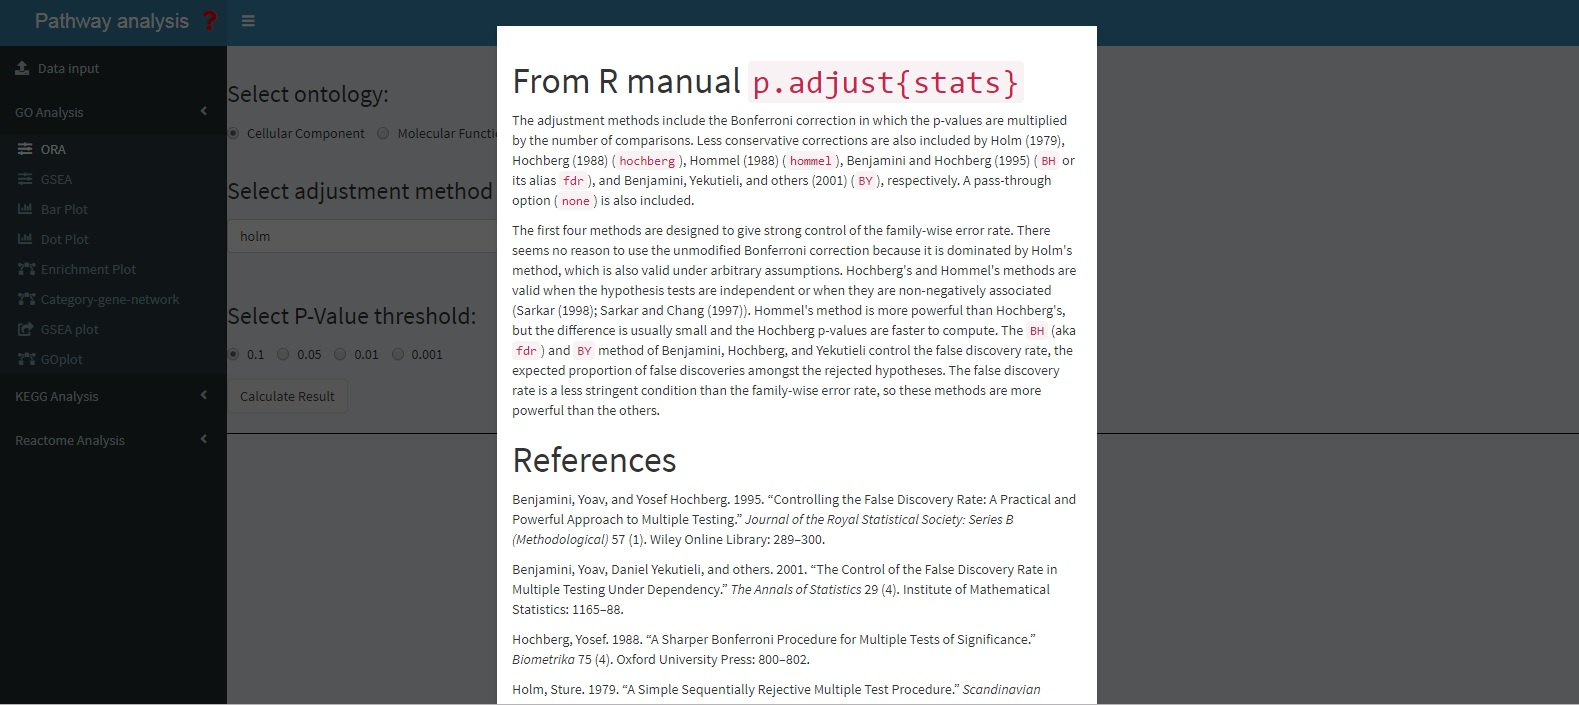
\includegraphics[width=0.9\textwidth]{figures/Help_pAdjustMethod.jpg} 
\caption{Ajuda per la selecció del mètode d'ajustament}
\end{figure}


\begin{figure}[H]
\centering
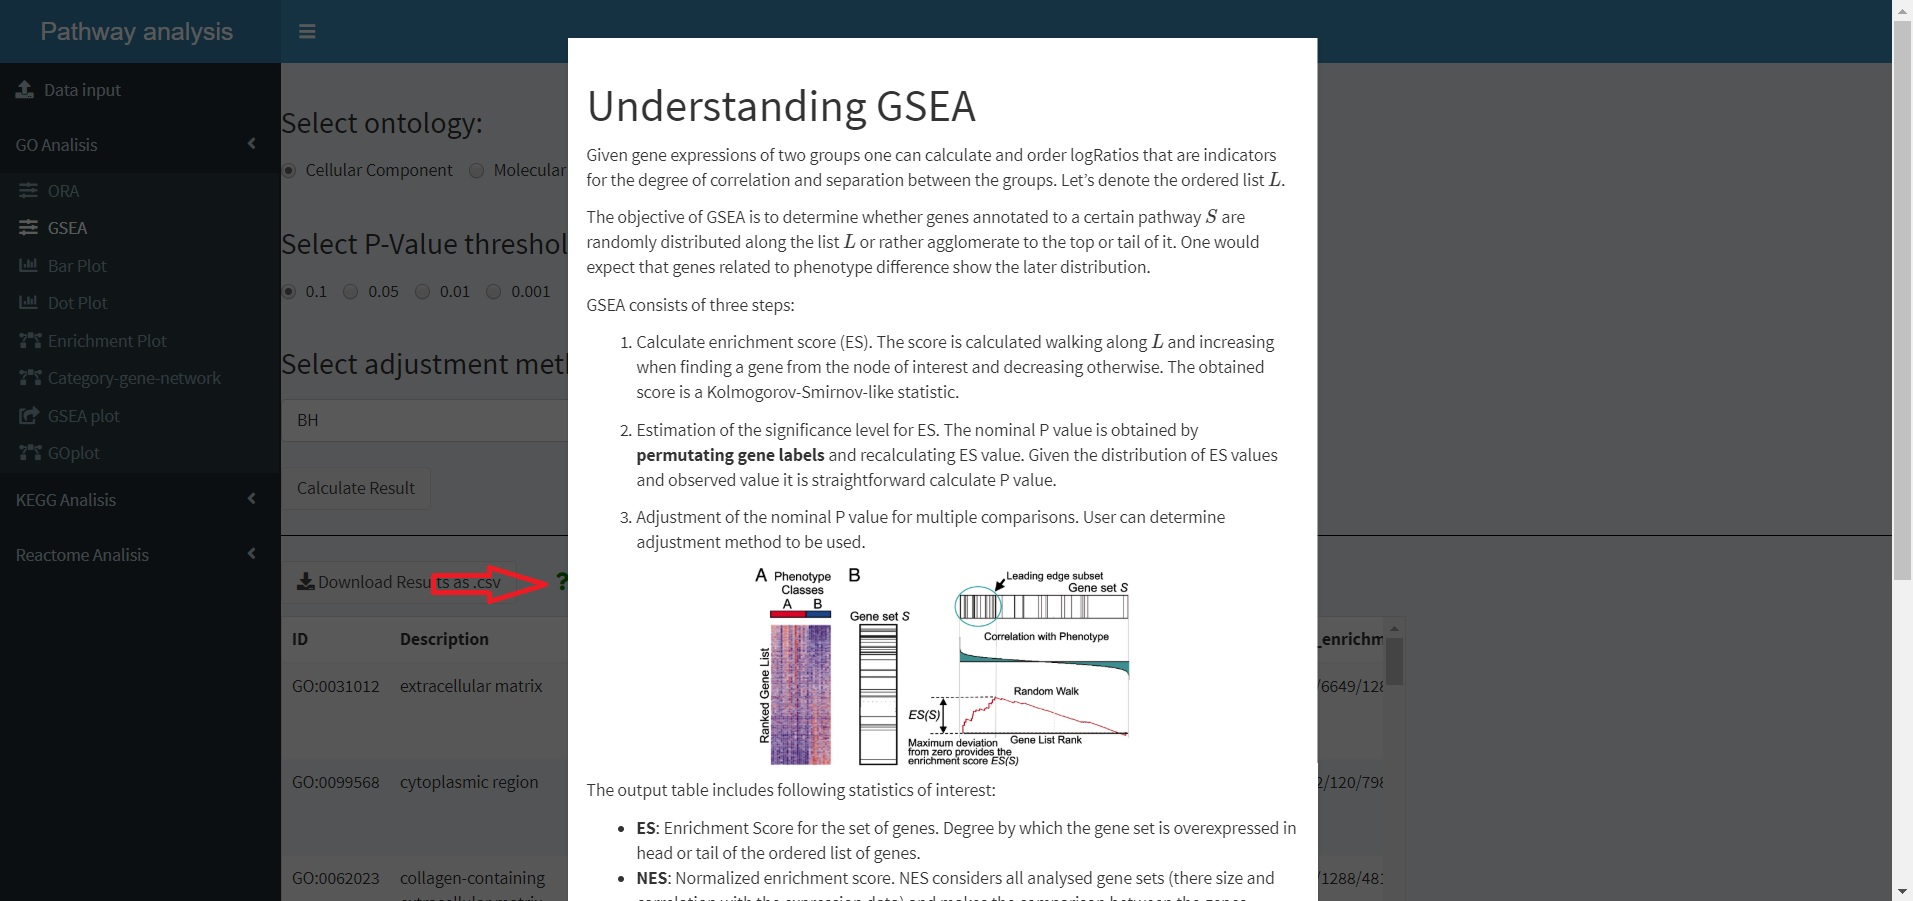
\includegraphics[width=0.9\textwidth]{figures/Help_GSEA_output.jpg} 
\caption{Ajuda per la interpretació de \gls{GSEA}}
\end{figure}


\chapter{Validació dels resultats}
\label{sec:ValRes}

L’anàlisi de les rutes representa l’últim pas de l’anàlisi d’expressions. Per dur a terme l’anàlisi de rutes és necessari tenir unes dades que ja estiguin processades prèviament (normalització, càlcul de les LogRatios, ajustament dels gens repetits a l’array, selecció dels gens diferencialment expressats, etc.). Les dades de \href{https://www.ncbi.nlm.nih.gov/geo/}{GEO (Gene Expression Omnibus)} estan però disponibles com a màxim en format normalitzat. Caldria doncs fer una anàlisi per arribar a un llistat de gens diferencialment expressats amb les logRatios per tots els gens de la mostra. Fer això no seria cap problema i de fet ho he fet per altres estudis. El problema és que arribo a resultats diferents dels resultats dels estudis d’on provenen les dades. Per tant les dades que entraria a l’aplicació serien diferents de les dades de l’estudi i lògicament amb aquesta comprovació no comprovo el que realment m’interessa. He procedit a contactar el meu professor per si tindria (o coneixeria) dades preprocessades fins a un llistat de gens amb logRatios i amb el set de gens diferencialment expressats, per tal que les pugui utilitzar en la meva aplicació. El meu professor m'ha redirigit, entre altres enllaços molt útils, al seu repositori a \href{https://github.com/alexsanchezpla?tab=repositories}{github.com}. 


\begin{table}[ht]
\centering
\begin{adjustbox}{width=1\textwidth}
\small
\begin{tabular}{||c | c | c | c | c ||} 
\hline 
Estudi & GEO ID & Espècie & Tipo d'experiment & Font \\ [0.5ex] 
\hline\hline
\cite{schmidt2008humoral} & \href{https://www.ncbi.nlm.nih.gov/geo/query/acc.cgi?acc=GSE11121}{GSE11121}& Homo sapiens & Microarrays & \href{https://bioconductor.org/packages/release/bioc/html/DOSE.html}{Paquet \helvetica{DOSE} de \gls{Bioconductor}}\\
\hline
\cite{li2017zbtb7b} & \href{https://www.ncbi.nlm.nih.gov/geo/query/acc.cgi?acc=GSE100924}{GSE100924}& Mus musculus & Microarrays & \href{https://github.com/alexsanchezpla/StatisticalAnalysisOfMicroarrayData}{Github Sanchez Pla} \\ 
\hline
\cite{farmer2005identification} & \href{https://www.ncbi.nlm.nih.gov/geo/query/acc.cgi?acc=GSE1561}{GSE1561}&Homo sapiens& Microarrays & \href{https://github.com/alexsanchezpla/Ejemplo_de_MDA_con_Bioconductor}{Github Sanchez Pla} \\ 
\hline
\cite{hengel2003cutting} & \href{https://david.ncifcrf.gov/helps/demo1.txt}{DAVID Demo List 1}&Homo sapiens& Microarrays & \href{https://david.ncifcrf.gov/content.jsp?file=FAQs.html}{DAVID} \\ 
\hline
\end{tabular}
\end{adjustbox}
\end{table} 

Les dades de \cite{schmidt2008humoral}, que s'utilitzen en els vignettes de \helvetica{clusterProfiler} i \helvetica{ReactomePA}, ja les he mostrat en gran part a dalt quan explicava el contingut de l'aplicació. Els resultats obtinguts amb l'aplicació són iguals als resultats en els vignettes mencionats. Procediré doncs amb l'exemple basat en les dades de \cite{li2017zbtb7b} .

\section{Exemple d'anàlisi 1. GEO: GSE100924}

\cite{li2017zbtb7b} analitzen l'associació del gen Zbtb7b amb la producció dels greixos marrons que al seu torn influeixen en termogènesis i processos metabòlics diferents. D'aquesta manera els greixos marrons són importants per al tractament dels desordres metabòlics.

Les dades d'estudi són ja preprocessades per Ricardo Gonzalo Sanz i Sanchez Pla i estan disponibles a \href{https://github.com/alexsanchezpla/StatisticalAnalysisOfMicroarrayData}{github}. De la carpeta \textit{results} he agafat la taula \textit{topAnnotated\_KOvsWT\_COLD.csv}. Sanz i Pla utilitzen el paquet \helvetica{ReactomePA} per a l'anàlisi d'enriquiment. Repeteixo doncs el seu anàlisi utilitzant l'aplicació. 


\begin{enumerate}

\item Elegeixo l'espècie \textit{Mus musculus} per a \gls{GO}, \gls{KEGG} i Reactome.
\begin{figure}[H]
\centering
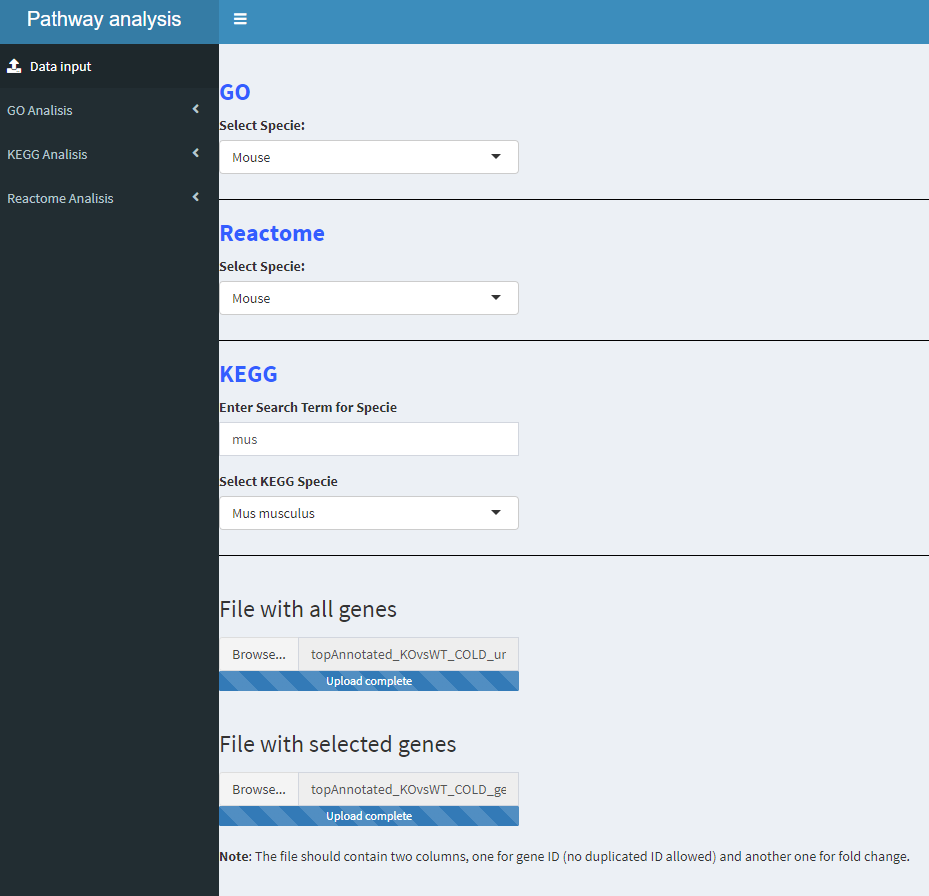
\includegraphics[width=0.6\textwidth]{figures/Estudi1_Fig1_Select_Specie.png} 
\caption{Selecció d'espècie}
\end{figure}

L'output a baix indica que s'ha pujat el total de 5995 gens. Per a l'arxiu dels gens seleccionats l'aplicació diu que s'han pujat 769 gens.

\begin{figure}[H]
\centering
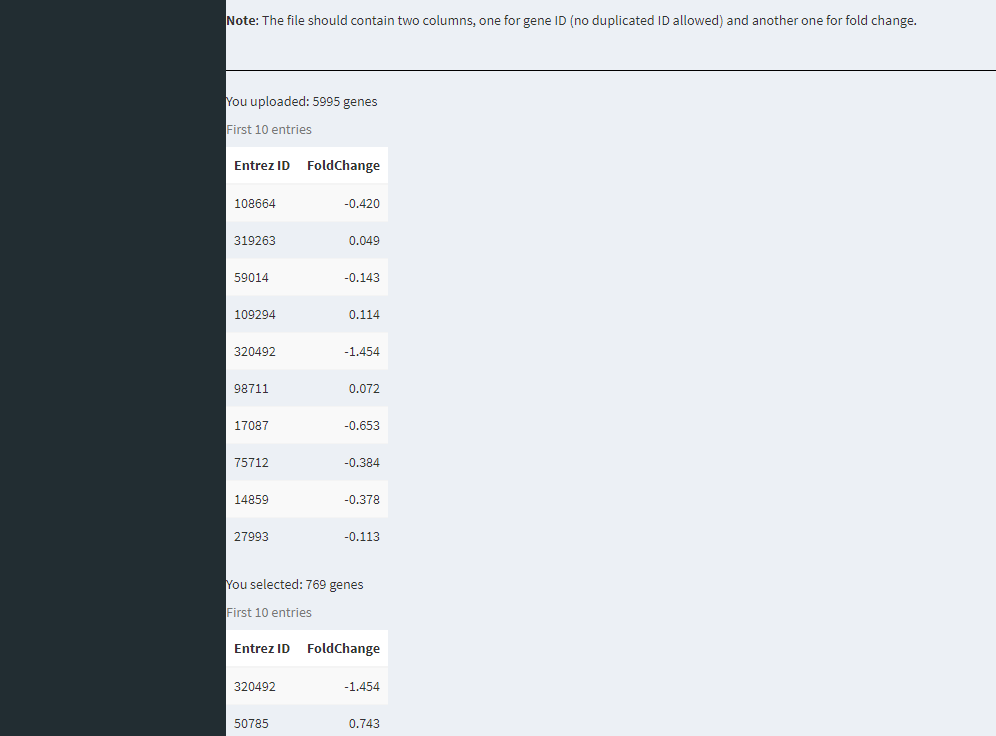
\includegraphics[width=0.6\textwidth]{figures/Estudi1_Fig2_Select_Specie.png} 
\caption{Breu resum de les dades}
\end{figure}


\item Clico en l'apartat \textit{Reactome Analysis}$\rightarrow$\textit{ORA}. Selecciono com a mètode d'ajustament \textit{BH} i el cut-off del valor de P ajustat 0.05. Clico a \textit{Calculate results}

\begin{figure}[H]
\centering
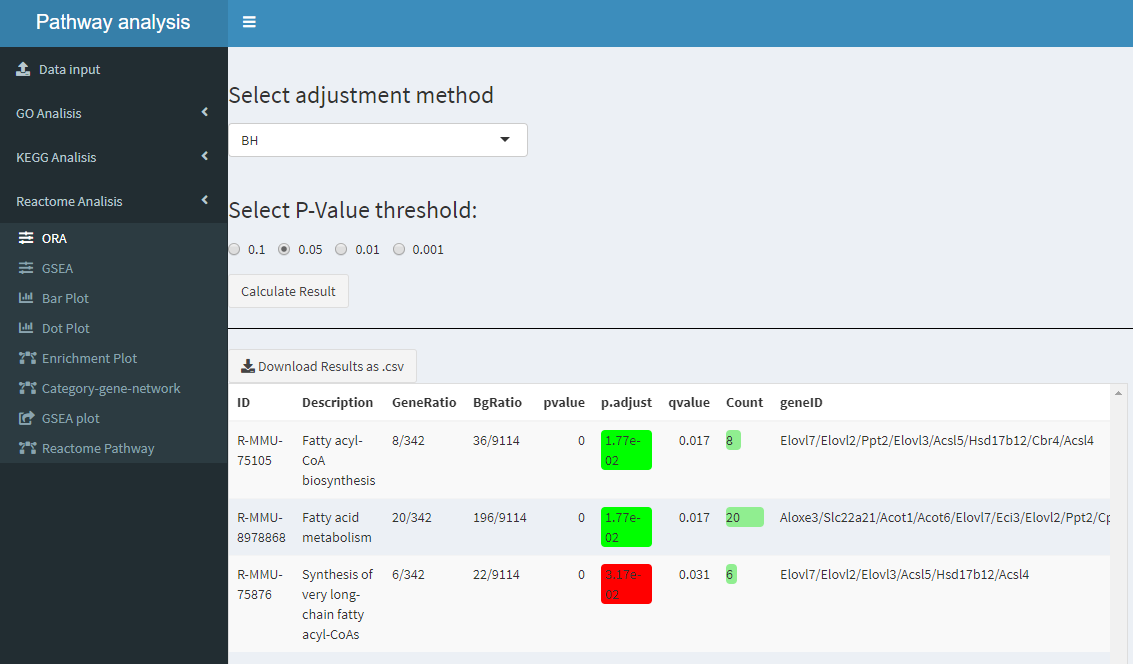
\includegraphics[width=0.6\textwidth]{figures/Estudi1_Fig3_ORA_RA.png} 
\caption{Resultat d'anàlisi ORA de Reactome}
\end{figure}

Observem que les rutes mostrades són les mateixes esmentades per Sanz i Pla. També destaquem que el resultat coincideix amb les trobades a l’estudi de \cite{li2017zbtb7b}. S'observa la pertorbació de les rutes relacionades amb els greixos marrons \textbf{Fatty acyl-CoA biosynthesis} i \textbf{Fatty-acid metabolism}.

\item Visualització del resultat \gls{ORA}

L'aplicació permet visualitzar els resultats obtinguts amb la \gls{ORA}. 

\begin{itemize}
\item Selecciono \textit{Reactome Analysis}$\rightarrow$\textit{Bar Plot}

\begin{figure}[H]
\centering
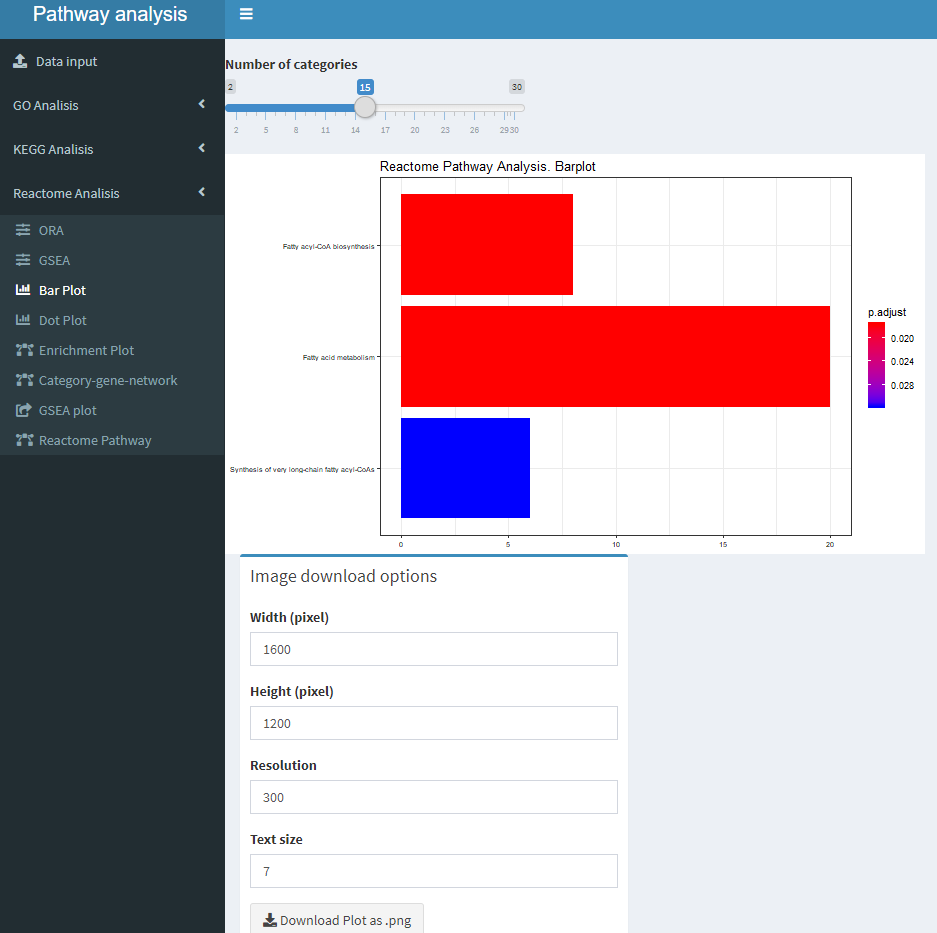
\includegraphics[width=0.6\textwidth]{figures/Estudi1_Fig4_ORA_BP_RA.png} 
\caption{Gràfic de barres}
\end{figure}

\item Selecciono \textit{Reactome Analysis}$\rightarrow$\textit{\gls{Dot-Plot}}

\begin{figure}[H]
\centering
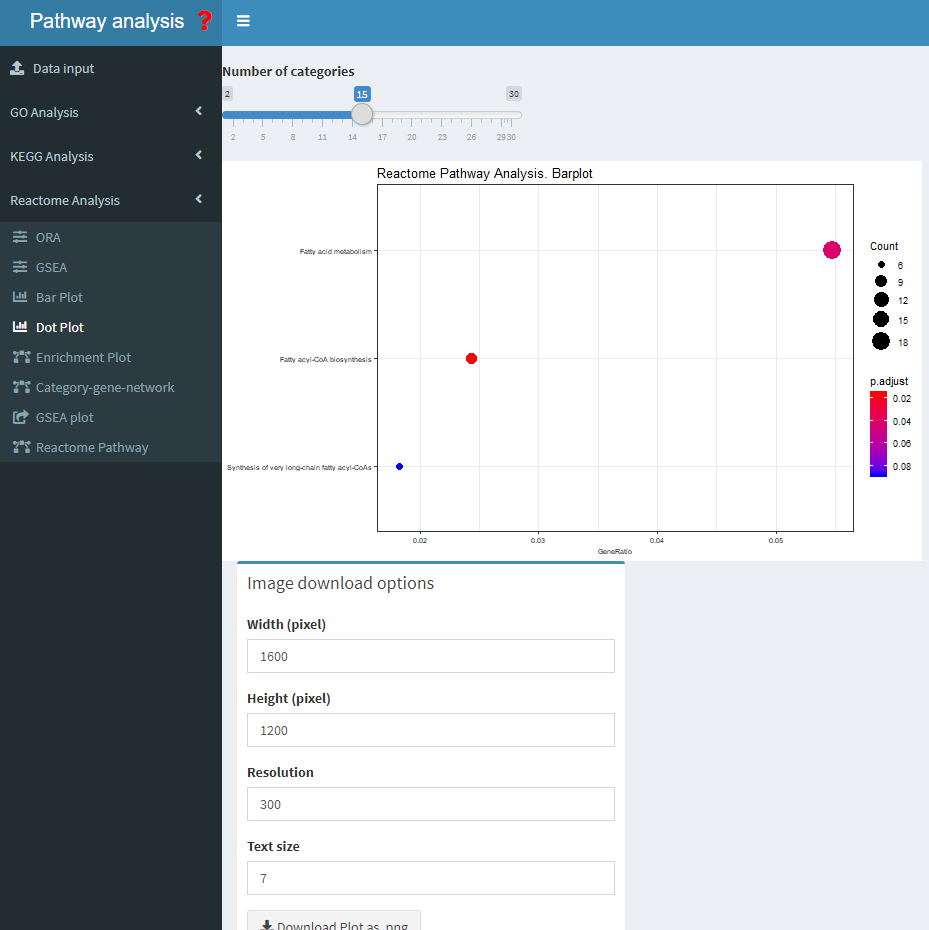
\includegraphics[width=0.6\textwidth]{figures/Estudi1_Fig5_ORA_Dot_RA.png} 
\caption{Gràfic de punts}
\end{figure}

\item Selecciono \textit{Reactome Analysis}$\rightarrow$\textit{\gls{Enrichment Map} Plot}

\begin{figure}[H]
\centering
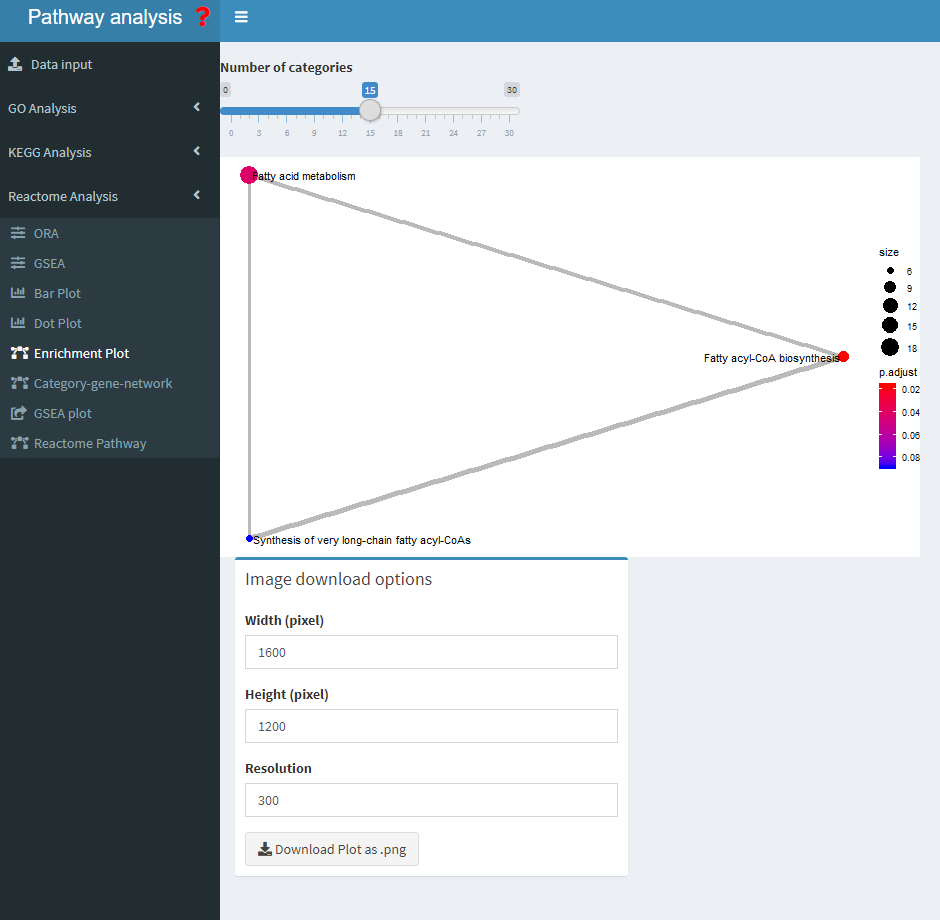
\includegraphics[width=0.6\textwidth]{figures/Estudi1_Fig6_ORA_EP_RA.png} 
\caption{Mapa d’enriquiment}
\end{figure}

Observem que totes les rutes identificades comparteixen els gens.

\item Selecciono \textit{Reactome Analysis}$\rightarrow$\textit{\gls{Gene-Concept-Network}}
Aquesta visualització incorpora els gens individuals de la ruta i la magnitud de la seva expressió diferencial. Observem que el gen Elovl3 està sotaexpressat, tal com es comenta al paper de \cite{li2017zbtb7b}. El gen Elovl3 és el component important per a reclutament dels lípids al teixit adipós marró \cite{westerberg2006elovl3}

\begin{figure}[H]
\centering
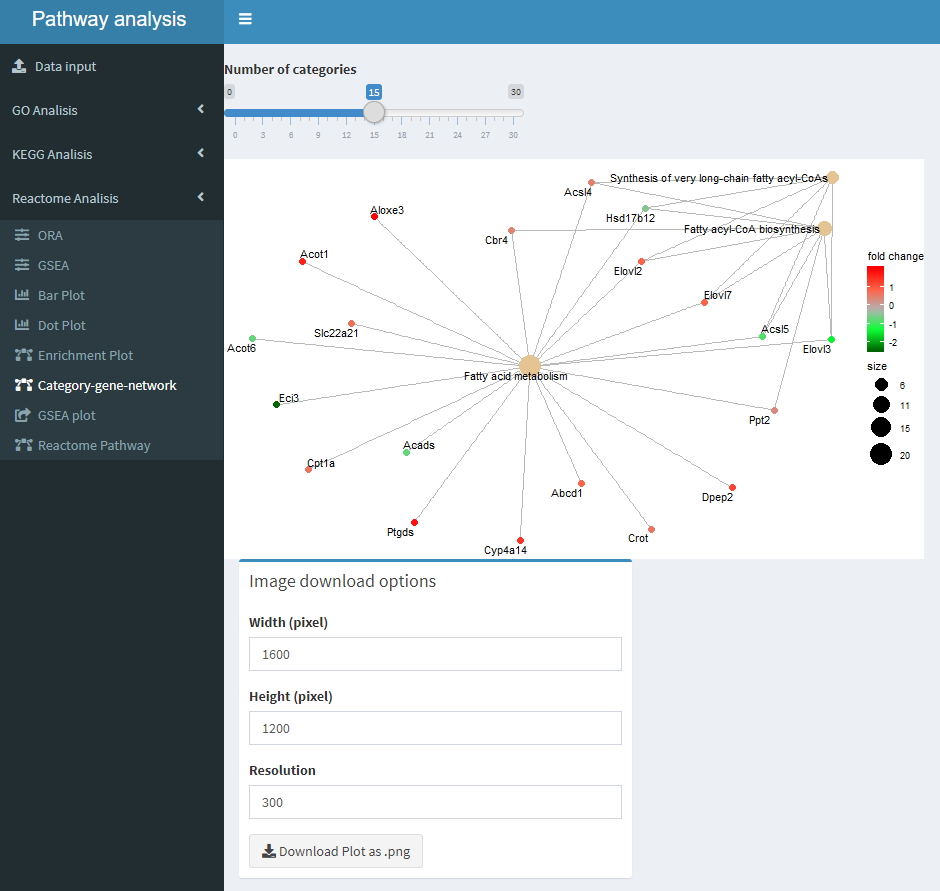
\includegraphics[width=0.6\textwidth]{figures/Estudi1_Fig7_ORA_CP_RA.png} 
\caption{Red de les categories i gens}
\end{figure}

\item Selecciono \textit{Reactome Analysis}$\rightarrow$\textit{Reactome Pathway}
\begin{figure}[H]
\centering
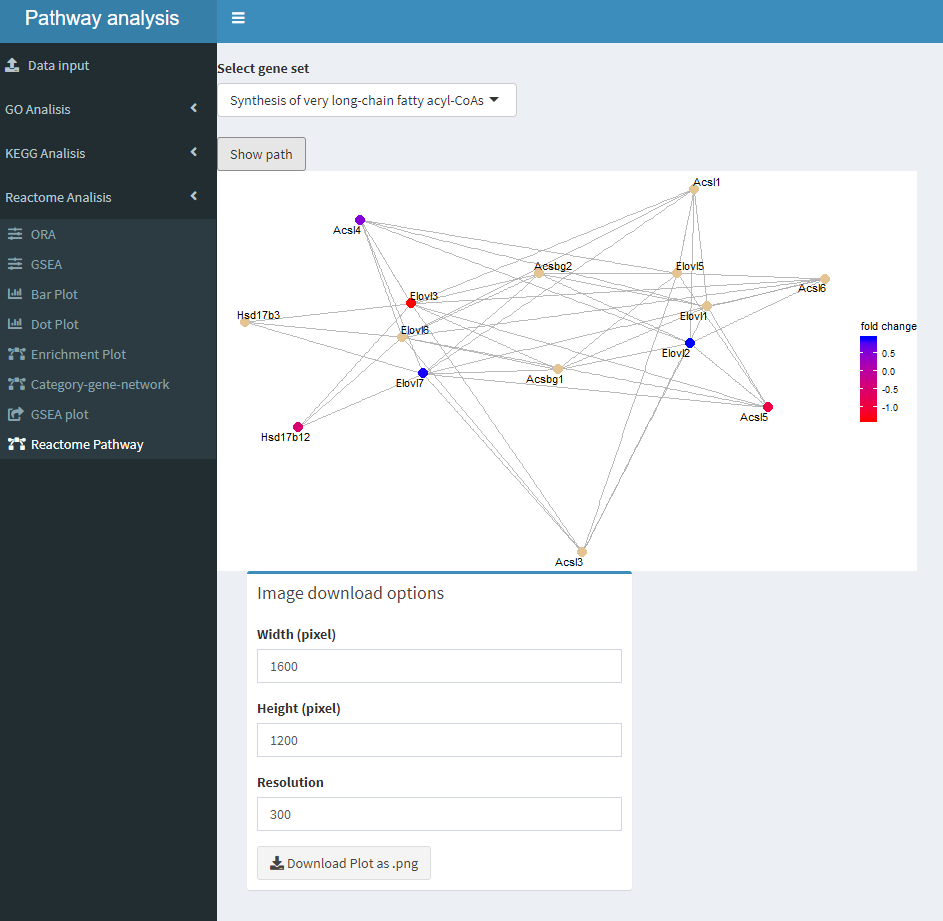
\includegraphics[width=0.6\textwidth]{figures/Estudi1_Fig8_ORA_PP_RA.png} 
\caption{Rutes Reactome}
\end{figure}
\end{itemize}
\end{enumerate}

Addicionalment a l'anàlisi \gls{ORA} podem fer, mitjançant l'aplicació, l'anàlisi \gls{GSEA} per les rutes de Reactome. Per fer-ho:

\begin{enumerate}

\item Clico en l'apartat \textit{Reactome Analysis}$\rightarrow$\textit{\gls{GSEA}}. Selecciono com a mètode d'ajustament \textit{BH} i el cut-off del valor de P ajustat 0.05. Clico a \textit{Calculate results}

Amb el valor de P de 0.05 l'anàlisi no troba cap ruta enriquida.

\item Augmento el Cut-Off del valor de P a 0.1

Amb el Cut-Off més alt l'aplicació retorna un llistat de gens.

\begin{figure}[H]
\centering
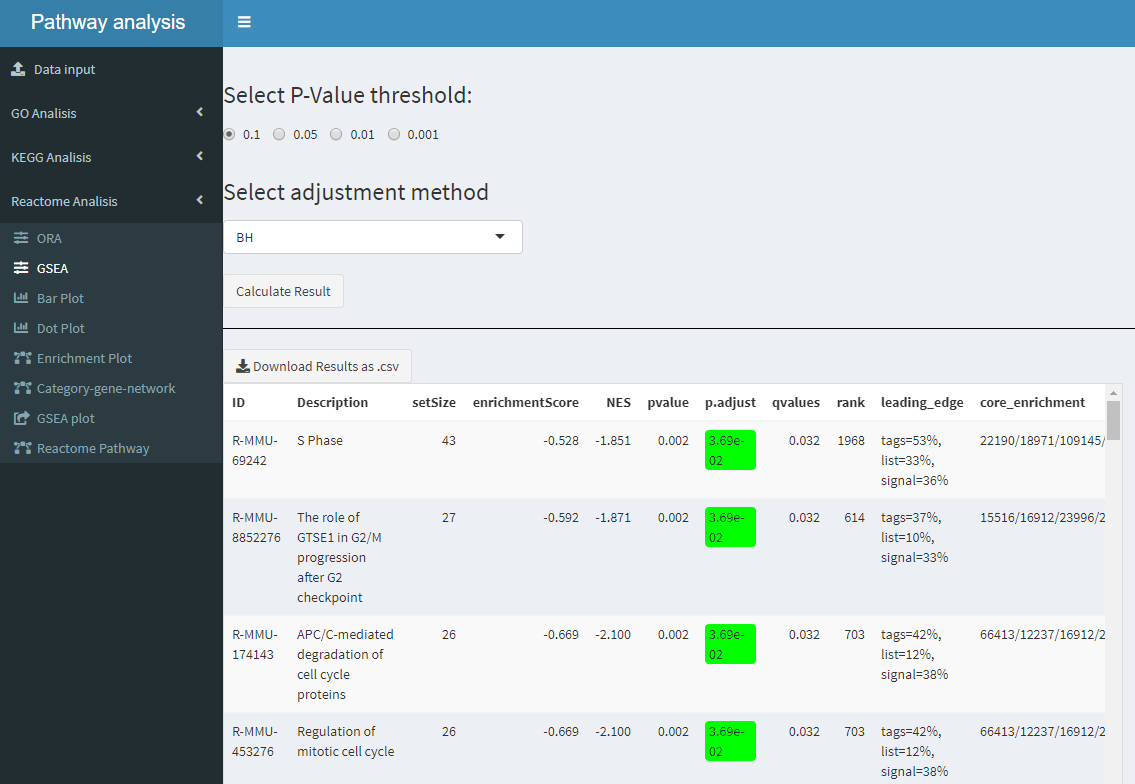
\includegraphics[width=0.6\textwidth]{figures/Estudi1_Fig9_GSEA_RA.png} 
\caption{Anàlisi GSEA}
\end{figure}

\item Per obtenir els gràfics \gls{GSEA} anem a \textit{Reactome Analysis}$\rightarrow$\textit{GSEA plot}

\begin{figure}[H]
\centering
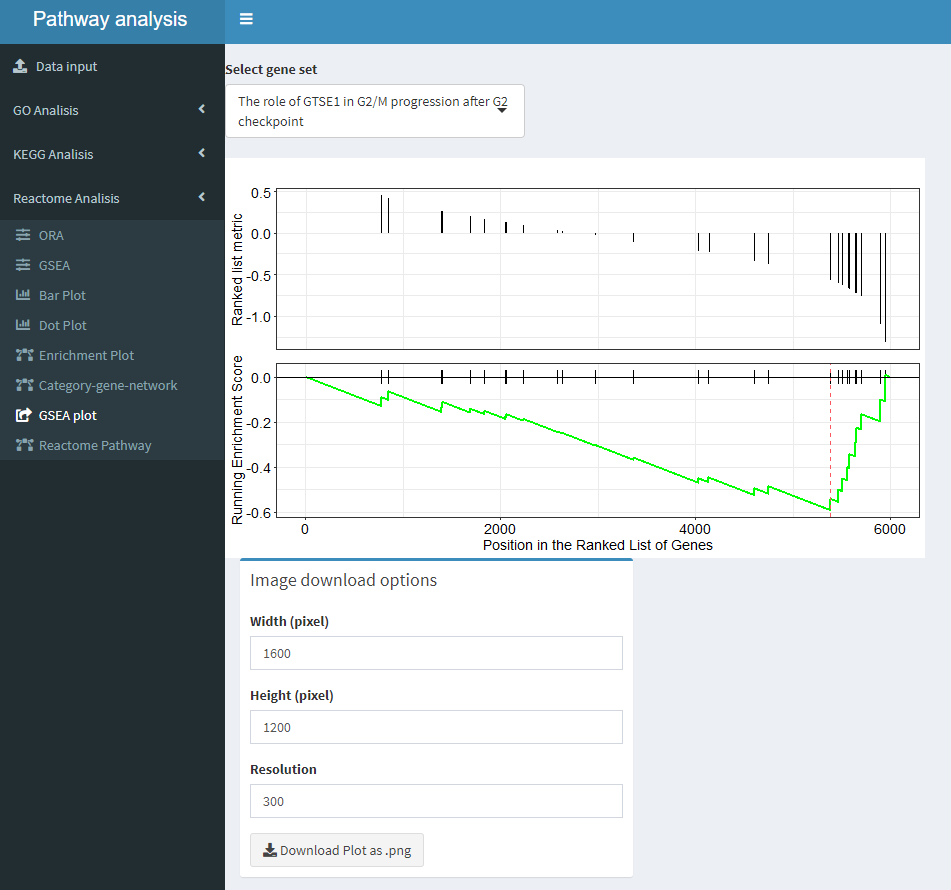
\includegraphics[width=0.6\textwidth]{figures/Estudi1_Fig10_GSEA_RA.png} 
\caption{Gràfic \gls{GSEA}}
\end{figure}
\end{enumerate}

També podem fer l'anàlisi de KEGG. El resultat de KEGG és similar a l'anàlisi de Reactome. L'aplicació permet però generar les rutes KEGG. Per obtenir-les:

\begin{enumerate}
\item Clico en l'apartat \textit{KEGG Analysis}$\rightarrow$\textit{ORA}. Selecciono com a mètode d'ajustament \textit{BH} i el cut-off del valor de P ajustat 0.05. Clico a \textit{Calculate results}
\begin{figure}[H]
\centering
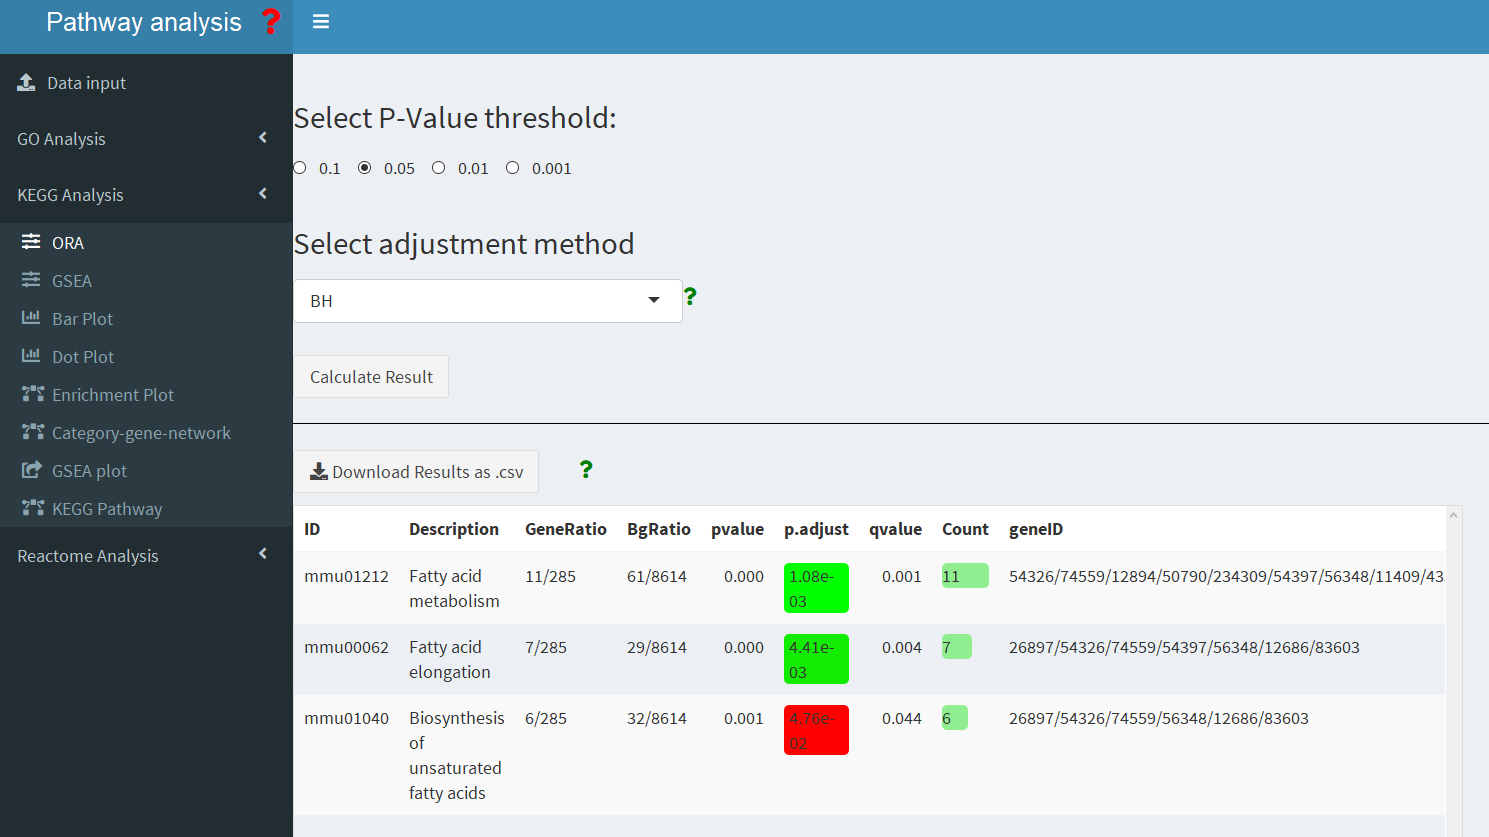
\includegraphics[width=0.6\textwidth]{figures/Estudi1_Fig11_ORA_KEGG.png} 
\caption{Anàlisi \gls{ORA} de \gls{KEGG}}
\end{figure}

\item Anem a \textit{KEGG}$\rightarrow$\textit{\gls{KEGG Pathway}}
\begin{figure}[H]
\centering
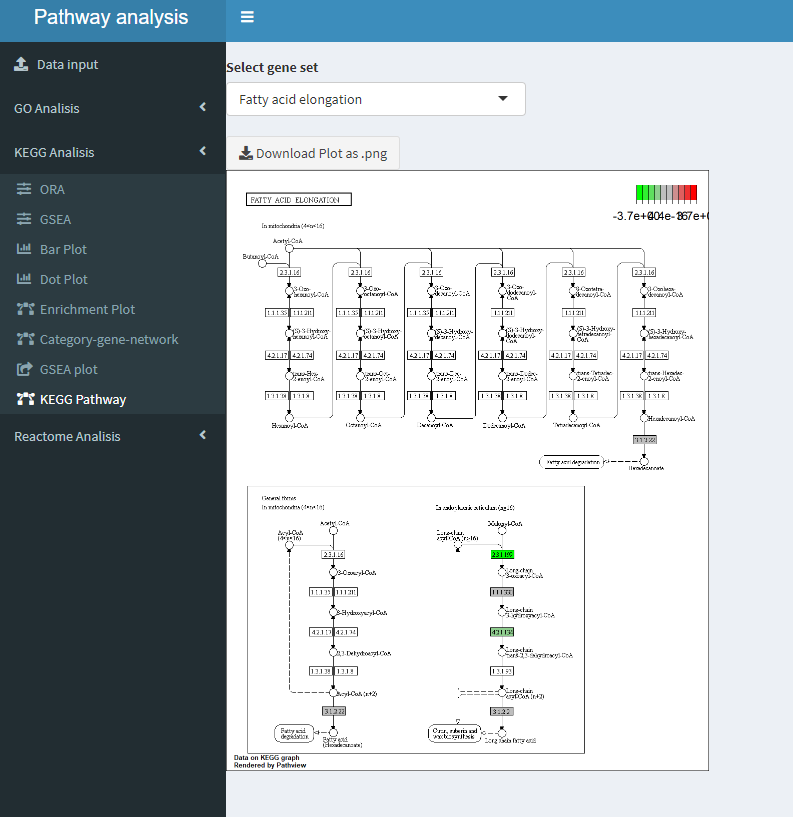
\includegraphics[width=0.6\textwidth]{figures/Estudi1_Fig12_KEGG_Pathway.png} 
\caption{Gràfic de les rutes \gls{KEGG}}
\end{figure}
\end{enumerate}

L'anàlisi GO no retorna cap terme GO amb el nivell de significació de 0.05. Pujant el nivell de significació fins 0.1 retorna un llistat dels termes enriquits per als components cel·lulars.

Clico en l'apartat \textit{\gls{GO} Analysis}$\rightarrow$\textit{ORA}. Selecciono com a mètode d'ajustament \textit{BH} i el cut-off del valor de P ajustat 0.1. Selecciono també \textit{CC}. Clico a \textit{Calculate results}
\begin{figure}[H]
\centering
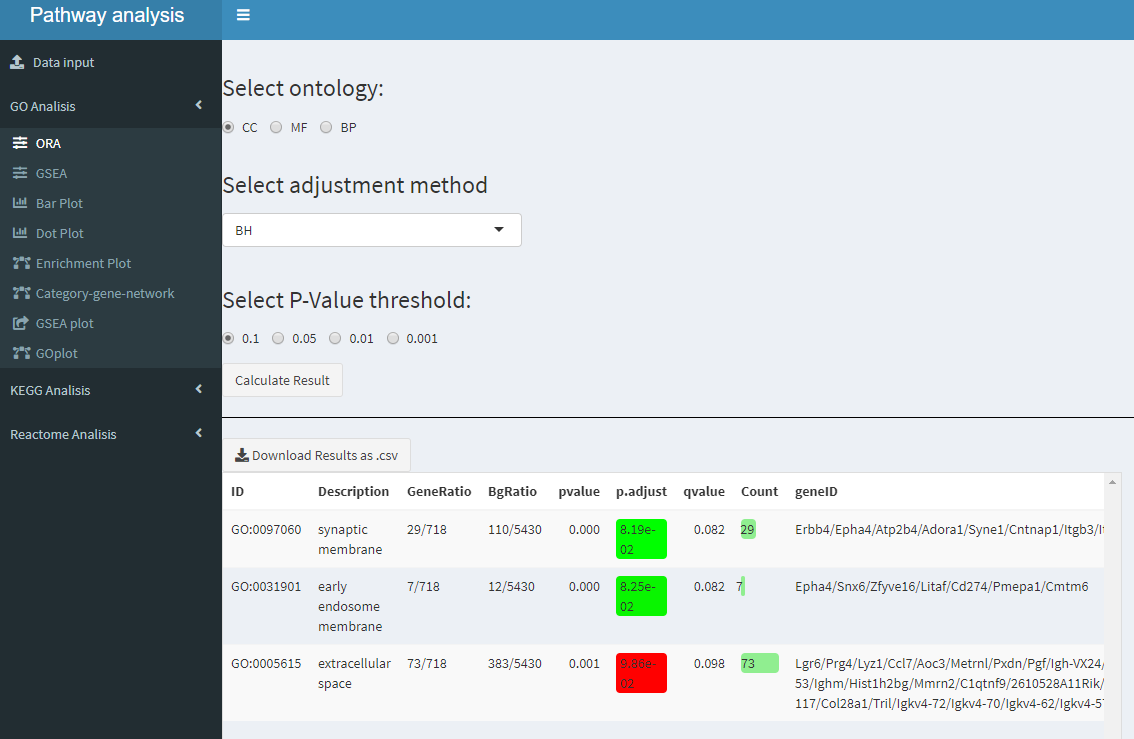
\includegraphics[width=0.6\textwidth]{figures/Estudi1_Fig13_GO.png} 
\caption{L'anàlisi \gls{ORA} de \gls{GO}}
\end{figure}

\chapter{Conclusions}

Al treball final he tingut com a objectiu la creació d'una aplicació per a l’anàlisi de les rutes. Primer he determinat què és l'anàlisi de les rutes i on se situa en l'anàlisi global d'expressió genètica. He explicat que l'anàlisi de les rutes és l'últim pas de l'anàlisi d'expressió gènica on es pretén donar sentit biològic a les dades d'expressió. Per dur a terme aquesta anàlisi s'utilitza una llista dels gens diferencialment expressats i els \gls{logRatio}s de tots els gens de l'experiment. Així, he explicat que es necessari anotar aquests gens a les bases existents per poder agrupar-los en conceptes (o rutes). 

En segon lloc, he triat les bases de dades més conegudes i que són utilitzades pels paquets de \gls{Bioconductor}. Aquestes bases de dades són: \gls{GO}, \gls{KEGG} i Reactome. En tercer lloc, he descrit quins mètodes existeixen per calcular la significació biològica de les rutes. Entre altres he identificat tres estratègies: \gls{ORA}, \gls{FCS} i l'anàlisi topològic de les rutes. En quart lloc, he descrit amb més detall els mètodes \gls{ORA} i \gls{GSEA} i també he identificat les possibilitats per visualitzar les rutes. En cinquè lloc, després de formular un protocol d'anàlisi, he buscat i identificat els paquets de \gls{Bioconductor} que permeten aplicar els mètodes descrits. Entre altres he triat \helvetica{clusterProfiler}, \helvetica{ReactomePA} i \helvetica{pathview}. He posat aquests paquets com a base per la futura aplicació. 

El resultat ha estat l'aplicació dividida en quatre apartats: 1) Entrada de les dades; 2) Anàlisi amb la base d'anotació GO; 3) Anàlisi amb la base d'anotació \gls{KEGG} i anàlisi amb la base d'anotació Reactome. Per a cada base de dades l'usuari pot fer \gls{ORA}, \gls{GSEA} i obtenir la visualització de la topologia de les rutes. L'aplicació permet descarregar els resultats com a arxiu .csv i imatges .png, els quals l'usuari pot personalitzar. 
Pel que fa a la validació dels resultats, s’ha mostrat una bona coincidència amb l'estudi triat per validar les dades. Aquest estudi investiga l'impacte del gen Zbtb7b sobre la producció dels greixos marrons. Justament les rutes relacionades amb la síntesi de greixos marrons estaven identificades amb l'aplicació. En darrer lloc, l'aplicació pot ser descarregada i instal·lada lliurement del repositori GitHub i la via per fer-ho s'explica a la memòria. Actualment es busca el mètode per publicar l'aplicació a internet per fer-la encara més accessible.


